\documentclass[]{article}
\usepackage{lmodern}
\usepackage{amssymb,amsmath}
\usepackage{ifxetex,ifluatex}
\usepackage{fixltx2e} % provides \textsubscript
\ifnum 0\ifxetex 1\fi\ifluatex 1\fi=0 % if pdftex
  \usepackage[T1]{fontenc}
  \usepackage[utf8]{inputenc}
\else % if luatex or xelatex
  \ifxetex
    \usepackage{mathspec}
  \else
    \usepackage{fontspec}
  \fi
  \defaultfontfeatures{Ligatures=TeX,Scale=MatchLowercase}
  \newcommand{\euro}{€}
\fi
% use upquote if available, for straight quotes in verbatim environments
\IfFileExists{upquote.sty}{\usepackage{upquote}}{}
% use microtype if available
\IfFileExists{microtype.sty}{%
\usepackage{microtype}
\UseMicrotypeSet[protrusion]{basicmath} % disable protrusion for tt fonts
}{}


\setlength{\parindent}{0pt}
\setlength{\parskip}{6pt plus 2pt minus 1pt}
\setlength{\emergencystretch}{3em}  % prevent overfull lines
\providecommand{\tightlist}{%
  \setlength{\itemsep}{0pt}\setlength{\parskip}{0pt}}
\setcounter{secnumdepth}{5}

%%% Use protect on footnotes to avoid problems with footnotes in titles
\let\rmarkdownfootnote\footnote%
\def\footnote{\protect\rmarkdownfootnote}

%%% Change title format to be more compact
\usepackage{titling}

\RequirePackage[]{C:/Users/Davoud68/Documents/R/win-library/3.3/BiocStyle/resources/tex/Bioconductor2}

% Create subtitle command for use in maketitle
\newcommand{\subtitle}[1]{
  \posttitle{
    \begin{center}\large#1\end{center}
    }
}

\setlength{\droptitle}{-2em}
  \title{Intermediate R}
  \pretitle{\vspace{\droptitle}\centering\huge}
  \posttitle{\par}
  \author{}
  \preauthor{}\postauthor{}
  \date{}
  \predate{}\postdate{}


% Redefines (sub)paragraphs to behave more like sections
\ifx\paragraph\undefined\else
\let\oldparagraph\paragraph
\renewcommand{\paragraph}[1]{\oldparagraph{#1}\mbox{}}
\fi
\ifx\subparagraph\undefined\else
\let\oldsubparagraph\subparagraph
\renewcommand{\subparagraph}[1]{\oldsubparagraph{#1}\mbox{}}
\fi

% code highlighting
\definecolor{fgcolor}{rgb}{0.251, 0.251, 0.251}
\newcommand{\hlnum}[1]{\textcolor[rgb]{0.816,0.125,0.439}{#1}}%
\newcommand{\hlstr}[1]{\textcolor[rgb]{0.251,0.627,0.251}{#1}}%
\newcommand{\hlcom}[1]{\textcolor[rgb]{0.502,0.502,0.502}{\textit{#1}}}%
\newcommand{\hlopt}[1]{\textcolor[rgb]{0,0,0}{#1}}%
\newcommand{\hlstd}[1]{\textcolor[rgb]{0.251,0.251,0.251}{#1}}%
\newcommand{\hlkwa}[1]{\textcolor[rgb]{0.125,0.125,0.941}{#1}}%
\newcommand{\hlkwb}[1]{\textcolor[rgb]{0,0,0}{#1}}%
\newcommand{\hlkwc}[1]{\textcolor[rgb]{0.251,0.251,0.251}{#1}}%
\newcommand{\hlkwd}[1]{\textcolor[rgb]{0.878,0.439,0.125}{#1}}%
\let\hlipl\hlkwb
%
\usepackage{fancyvrb}
\newcommand{\VerbBar}{|}
\newcommand{\VERB}{\Verb[commandchars=\\\{\}]}
\DefineVerbatimEnvironment{Highlighting}{Verbatim}{commandchars=\\\{\}}
%
\newenvironment{Shaded}{\begin{myshaded}}{\end{myshaded}}
% set background for result chunks
\let\oldverbatim\verbatim
\renewenvironment{verbatim}{\color{codecolor}\begin{myshaded}\begin{oldverbatim}}{\end{oldverbatim}\end{myshaded}}
%
\newcommand{\KeywordTok}[1]{\hlkwd{#1}}
\newcommand{\DataTypeTok}[1]{\hlkwc{#1}}
\newcommand{\DecValTok}[1]{\hlnum{#1}}
\newcommand{\BaseNTok}[1]{\hlnum{#1}}
\newcommand{\FloatTok}[1]{\hlnum{#1}}
\newcommand{\CharTok}[1]{\hlstr{#1}}
\newcommand{\StringTok}[1]{\hlstr{#1}}
\newcommand{\CommentTok}[1]{\hlcom{#1}}
\newcommand{\OtherTok}[1]{{#1}}
\newcommand{\AlertTok}[1]{\textcolor[rgb]{0.94,0.16,0.16}{{#1}}}
\newcommand{\FunctionTok}[1]{\textcolor[rgb]{0.00,0.00,0.00}{{#1}}}
\newcommand{\RegionMarkerTok}[1]{{#1}}
\newcommand{\ErrorTok}[1]{\textbf{{#1}}}
\newcommand{\NormalTok}[1]{\hlstd{#1}}
%
\AtBeginDocument{\bibliographystyle{C:/Users/Davoud68/Documents/R/win-library/3.3/BiocStyle/resources/tex/unsrturl}}

\begin{document}
\maketitle

{
\setcounter{tocdepth}{2}
\tableofcontents
\newpage
}
\section{Required packages and other
preparations}\label{required-packages-and-other-preparations}

\begin{Shaded}
\begin{Highlighting}[]
\KeywordTok{library}\NormalTok{(}\StringTok{"TeachingDemos"}\NormalTok{)}
\KeywordTok{library}\NormalTok{(}\StringTok{"openxlsx"}\NormalTok{)}
\KeywordTok{library}\NormalTok{(}\StringTok{"multtest"}\NormalTok{)}
\KeywordTok{library}\NormalTok{(}\StringTok{"Biobase"}\NormalTok{)}
\KeywordTok{library}\NormalTok{(}\StringTok{"tidyverse"}\NormalTok{)}
\KeywordTok{library}\NormalTok{(}\StringTok{"cowplot"}\NormalTok{)}
\end{Highlighting}
\end{Shaded}

\section{Conditionals and Control
Flow}\label{conditionals-and-control-flow}

\subsection{Relational Operators}\label{relational-operators}

The most basic form of comparison is equality. Let's briefly recap its
syntax. The following statements all evaluate to TRUE (feel free to try
them out in the console).

\begin{Shaded}
\begin{Highlighting}[]
\DecValTok{3} \OperatorTok{==}\StringTok{ }\NormalTok{(}\DecValTok{2} \OperatorTok{+}\StringTok{ }\DecValTok{1}\NormalTok{)}
\StringTok{"intermediate"} \OperatorTok{!=}\StringTok{ "r"}
\OtherTok{TRUE} \OperatorTok{!=}\StringTok{ }\OtherTok{FALSE}
\StringTok{"Rchitect"} \OperatorTok{!=}\StringTok{ "rchitect"}
\end{Highlighting}
\end{Shaded}

Notice from the last expression that R is \textbf{case sensitive}: ``R''
is not equal to ``r''. Keep this in mind when solving the exercises in
this chapter!

\textbf{Instructions}

\begin{Shaded}
\begin{Highlighting}[]

\OperatorTok{*}\StringTok{ }\NormalTok{In the editor on the right, write R code to see }\ControlFlowTok{if} \StringTok{`}\DataTypeTok{TRUE}\StringTok{`}\NormalTok{ equals }\StringTok{`}\DataTypeTok{FALSE}\StringTok{`}\NormalTok{.}

\OperatorTok{*}\StringTok{ }\NormalTok{Likewise, check }\ControlFlowTok{if} \StringTok{`}\DataTypeTok{-6 * 14}\StringTok{`}\NormalTok{ is not equal to }\StringTok{`}\DataTypeTok{17 - 101}\StringTok{`}\NormalTok{.}

\OperatorTok{*}\StringTok{ }\NormalTok{Next up}\OperatorTok{:}\StringTok{ }\NormalTok{comparison of character strings. Ask R whether the strings }\StringTok{"useR"}\NormalTok{ and }\StringTok{"user"}\NormalTok{ are equal.}

\OperatorTok{*}\StringTok{ }\NormalTok{Finally, find out what happens }\ControlFlowTok{if}\NormalTok{ you compare logicals to numerics}\OperatorTok{:}\StringTok{ }\NormalTok{are }\StringTok{`}\DataTypeTok{TRUE}\StringTok{`}\NormalTok{ and }\DecValTok{1}\NormalTok{ equal?}
\end{Highlighting}
\end{Shaded}

\textbf{Answers}

\begin{Shaded}
\begin{Highlighting}[]
\CommentTok{# Comparison of logicals}
\OtherTok{TRUE} \OperatorTok{==}\StringTok{ }\OtherTok{FALSE}
\NormalTok{   [}\DecValTok{1}\NormalTok{] }\OtherTok{FALSE}

\CommentTok{# Comparison of numerics}
\OperatorTok{-}\DecValTok{6} \OperatorTok{*}\StringTok{ }\DecValTok{14} \OperatorTok{!=}\StringTok{ }\DecValTok{17} \OperatorTok{-}\StringTok{ }\DecValTok{101}
\NormalTok{   [}\DecValTok{1}\NormalTok{] }\OtherTok{FALSE}

\CommentTok{# Comparison of character strings}
\StringTok{"useR"} \OperatorTok{==}\StringTok{ "user"}
\NormalTok{   [}\DecValTok{1}\NormalTok{] }\OtherTok{FALSE}

\CommentTok{# Compare a logical with a numeric}
\OtherTok{TRUE} \OperatorTok{==}\StringTok{ }\DecValTok{1}
\NormalTok{   [}\DecValTok{1}\NormalTok{] }\OtherTok{TRUE}
\end{Highlighting}
\end{Shaded}

Awesome! Since TRUE coerces to 1 under the hood, TRUE == 1 evaluates to
TRUE. Make sure not to mix up == (comparison) and = (assignment), == is
what need to check the equality of R objects.

\textbf{Greater and less than} Apart from equality operators, Filip also
introduced the less than and greater than operators:
\texttt{\textless{}} and \texttt{\textgreater{}}. You can also add an
equal sign to express less than or equal to or greater than or equal to,
respectively. Have a look at the following R expressions, that all
evaluate to \texttt{FALSE}:

\begin{Shaded}
\begin{Highlighting}[]
\NormalTok{(}\DecValTok{1} \OperatorTok{+}\StringTok{ }\DecValTok{2}\NormalTok{) }\OperatorTok{>}\StringTok{ }\DecValTok{4}
\StringTok{"dog"} \OperatorTok{<}\StringTok{ "Cats"}
\OtherTok{TRUE} \OperatorTok{<=}\StringTok{ }\OtherTok{FALSE}
\end{Highlighting}
\end{Shaded}

Remember that for string comparison, R determines the greater than
relationship based on alphabetical order. Also, keep in mind that
\texttt{TRUE} corresponds to \texttt{1} in R, and \texttt{FALSE} coerces
to 0 behind the scenes. Therefore, \texttt{FALSE\ \textless{}\ TRUE} is
\texttt{TRUE}.

\textbf{Instructions}

\begin{Shaded}
\begin{Highlighting}[]
\NormalTok{Write R expressions to check whether}\OperatorTok{:}

\ErrorTok{*}\StringTok{ `}\DataTypeTok{-6 * 5 + 2}\StringTok{`}\NormalTok{ is greater than or equal to }\StringTok{`}\DataTypeTok{-10 + 1}\StringTok{`}\NormalTok{.}
\OperatorTok{*}\StringTok{ "raining"}\NormalTok{ is less than or equal to }\StringTok{"raining dogs"}\NormalTok{.}
\OperatorTok{*}\StringTok{ }\OtherTok{TRUE}\NormalTok{ is greater than FALSE.}
\end{Highlighting}
\end{Shaded}

\textbf{Answers}

\begin{Shaded}
\begin{Highlighting}[]
\CommentTok{# Comparison of numerics}
\OperatorTok{-}\DecValTok{6} \OperatorTok{*}\StringTok{ }\DecValTok{5} \OperatorTok{+}\DecValTok{2} \OperatorTok{>=}\StringTok{ }\OperatorTok{-}\DecValTok{10} \OperatorTok{+}\StringTok{ }\DecValTok{1}
\NormalTok{   [}\DecValTok{1}\NormalTok{] }\OtherTok{FALSE}

\CommentTok{# Comparison of character strings}
\StringTok{"raining"} \OperatorTok{<=}\StringTok{ "raining dogs"}
\NormalTok{   [}\DecValTok{1}\NormalTok{] }\OtherTok{TRUE}

\CommentTok{# Comparison of logicals}
\OtherTok{TRUE} \OperatorTok{>}\StringTok{ }\OtherTok{FALSE}
\NormalTok{   [}\DecValTok{1}\NormalTok{] }\OtherTok{TRUE}
\end{Highlighting}
\end{Shaded}

Great job! Make sure to have a look at the console output to see if R
returns the results you expected.

\textbf{Compare vectors} ou are already aware that R is very good with
vectors. Without having to change anything about the syntax, R's
relational operators also work on vectors.

Let's go back to the example that was started in the video. You want to
figure out whether your activity on social media platforms have paid off
and decide to look at your results for LinkedIn and Facebook. The sample
code in the editor initializes the vectors linkedin and facebook. Each
of the vector contains the number of profile views your LinkedIn and
Facebook profiles had over the last seven days.

\textbf{Instructions}

\begin{Shaded}
\begin{Highlighting}[]
\NormalTok{Using relational operators, find a logical answer, i.e. }\StringTok{`}\DataTypeTok{TRUE}\StringTok{`}\NormalTok{ or }\StringTok{`}\DataTypeTok{FALSE}\StringTok{`}\NormalTok{, }\ControlFlowTok{for}\NormalTok{ the following questions}\OperatorTok{:}

\ErrorTok{*}\StringTok{ }\NormalTok{On which days did the number of LinkedIn profile views exceed }\DecValTok{15}\NormalTok{?}
\OperatorTok{*}\StringTok{ }\NormalTok{When was your LinkedIn profile viewed only }\DecValTok{5}\NormalTok{ times or fewer?}
\OperatorTok{*}\StringTok{ }\NormalTok{When was your LinkedIn profile visited more often than your Facebook profile?}
\end{Highlighting}
\end{Shaded}

\textbf{Answers}

\begin{Shaded}
\begin{Highlighting}[]
\CommentTok{# The linkedin and facebook vectors have already been created for you}
\NormalTok{linkedin <-}\StringTok{ }\KeywordTok{c}\NormalTok{(}\DecValTok{16}\NormalTok{, }\DecValTok{9}\NormalTok{, }\DecValTok{13}\NormalTok{, }\DecValTok{5}\NormalTok{, }\DecValTok{2}\NormalTok{, }\DecValTok{17}\NormalTok{, }\DecValTok{14}\NormalTok{)}
\NormalTok{facebook <-}\StringTok{ }\KeywordTok{c}\NormalTok{(}\DecValTok{17}\NormalTok{, }\DecValTok{7}\NormalTok{, }\DecValTok{5}\NormalTok{, }\DecValTok{16}\NormalTok{, }\DecValTok{8}\NormalTok{, }\DecValTok{13}\NormalTok{, }\DecValTok{14}\NormalTok{)}

\CommentTok{# Popular days}
\NormalTok{linkedin }\OperatorTok{>}\StringTok{ }\DecValTok{15}
\NormalTok{   [}\DecValTok{1}\NormalTok{]  }\OtherTok{TRUE} \OtherTok{FALSE} \OtherTok{FALSE} \OtherTok{FALSE} \OtherTok{FALSE}  \OtherTok{TRUE} \OtherTok{FALSE}

\CommentTok{# Quiet days}
\NormalTok{linkedin }\OperatorTok{<=}\StringTok{ }\DecValTok{5}
\NormalTok{   [}\DecValTok{1}\NormalTok{] }\OtherTok{FALSE} \OtherTok{FALSE} \OtherTok{FALSE}  \OtherTok{TRUE}  \OtherTok{TRUE} \OtherTok{FALSE} \OtherTok{FALSE}

\CommentTok{# LinkedIn more popular than Facebook}
\NormalTok{linkedin }\OperatorTok{>}\StringTok{ }\NormalTok{facebook}
\NormalTok{   [}\DecValTok{1}\NormalTok{] }\OtherTok{FALSE}  \OtherTok{TRUE}  \OtherTok{TRUE} \OtherTok{FALSE} \OtherTok{FALSE}  \OtherTok{TRUE} \OtherTok{FALSE}
\end{Highlighting}
\end{Shaded}

Wonderful! Have a look at the console output. Your LinkedIn profile was
pretty popular on the sixth day, but less so on the fourth and fifth
day.

\textbf{Compare matrices} R's ability to deal with different data
structures for comparisons does not stop at vectors. Matrices and
relational operators also work together seamlessly!

Instead of in vectors (as in the previous exercise), the LinkedIn and
Facebook data is now stored in a matrix called \texttt{views}. The first
row contains the LinkedIn information; the second row the Facebook
information. The original vectors \texttt{facebook} and
\texttt{linkedin} are still available as well.

\textbf{Instructions}

\begin{Shaded}
\begin{Highlighting}[]
\NormalTok{Using the relational operators you}\StringTok{'ve learned so far, try to discover the following:}

\StringTok{* When were the views exactly equal to 13? Use the `views` matrix to return a logical matrix.}
\StringTok{* For which days was the number of views less than or equal to 14? Again, have R return a logical matrix.}
\end{Highlighting}
\end{Shaded}

\textbf{Answers}

\begin{Shaded}
\begin{Highlighting}[]
\CommentTok{# The social data has been created for you}
\NormalTok{linkedin <-}\StringTok{ }\KeywordTok{c}\NormalTok{(}\DecValTok{16}\NormalTok{, }\DecValTok{9}\NormalTok{, }\DecValTok{13}\NormalTok{, }\DecValTok{5}\NormalTok{, }\DecValTok{2}\NormalTok{, }\DecValTok{17}\NormalTok{, }\DecValTok{14}\NormalTok{)}
\NormalTok{facebook <-}\StringTok{ }\KeywordTok{c}\NormalTok{(}\DecValTok{17}\NormalTok{, }\DecValTok{7}\NormalTok{, }\DecValTok{5}\NormalTok{, }\DecValTok{16}\NormalTok{, }\DecValTok{8}\NormalTok{, }\DecValTok{13}\NormalTok{, }\DecValTok{14}\NormalTok{)}
\NormalTok{views <-}\StringTok{ }\KeywordTok{matrix}\NormalTok{(}\KeywordTok{c}\NormalTok{(linkedin, facebook), }\DataTypeTok{nrow =} \DecValTok{2}\NormalTok{, }\DataTypeTok{byrow =} \OtherTok{TRUE}\NormalTok{)}

\CommentTok{# When does views equal 13?}
\NormalTok{views }\OperatorTok{==}\StringTok{ }\DecValTok{13}
\NormalTok{         [,}\DecValTok{1}\NormalTok{]  [,}\DecValTok{2}\NormalTok{]  [,}\DecValTok{3}\NormalTok{]  [,}\DecValTok{4}\NormalTok{]  [,}\DecValTok{5}\NormalTok{]  [,}\DecValTok{6}\NormalTok{]  [,}\DecValTok{7}\NormalTok{]}
\NormalTok{   [}\DecValTok{1}\NormalTok{,] }\OtherTok{FALSE} \OtherTok{FALSE}  \OtherTok{TRUE} \OtherTok{FALSE} \OtherTok{FALSE} \OtherTok{FALSE} \OtherTok{FALSE}
\NormalTok{   [}\DecValTok{2}\NormalTok{,] }\OtherTok{FALSE} \OtherTok{FALSE} \OtherTok{FALSE} \OtherTok{FALSE} \OtherTok{FALSE}  \OtherTok{TRUE} \OtherTok{FALSE}

\CommentTok{# When is views less than or equal to 14?}
\NormalTok{views }\OperatorTok{<=}\StringTok{ }\DecValTok{14}
\NormalTok{         [,}\DecValTok{1}\NormalTok{] [,}\DecValTok{2}\NormalTok{] [,}\DecValTok{3}\NormalTok{]  [,}\DecValTok{4}\NormalTok{] [,}\DecValTok{5}\NormalTok{]  [,}\DecValTok{6}\NormalTok{] [,}\DecValTok{7}\NormalTok{]}
\NormalTok{   [}\DecValTok{1}\NormalTok{,] }\OtherTok{FALSE} \OtherTok{TRUE} \OtherTok{TRUE}  \OtherTok{TRUE} \OtherTok{TRUE} \OtherTok{FALSE} \OtherTok{TRUE}
\NormalTok{   [}\DecValTok{2}\NormalTok{,] }\OtherTok{FALSE} \OtherTok{TRUE} \OtherTok{TRUE} \OtherTok{FALSE} \OtherTok{TRUE}  \OtherTok{TRUE} \OtherTok{TRUE}
\end{Highlighting}
\end{Shaded}

Nice job! This exercise concludes the part on comparators. Now that you
know how to query the relation between R objects, the next step will be
to use the results to alter the behavior of your programs.

\subsection{Logical Operators}\label{logical-operators}

\textbf{\& and \textbar{}} Before you work your way through the next
exercises, have a look at the following R expressions. All of them will
evaluate to TRUE:

\begin{Shaded}
\begin{Highlighting}[]
\OtherTok{TRUE} \OperatorTok{&}\StringTok{ }\OtherTok{TRUE}
\OtherTok{FALSE} \OperatorTok{|}\StringTok{ }\OtherTok{TRUE}
\DecValTok{5} \OperatorTok{<=}\StringTok{ }\DecValTok{5} \OperatorTok{&}\StringTok{ }\DecValTok{2} \OperatorTok{<}\StringTok{ }\DecValTok{3}
\DecValTok{3} \OperatorTok{<}\StringTok{ }\DecValTok{4} \OperatorTok{|}\StringTok{ }\DecValTok{7} \OperatorTok{<}\StringTok{ }\DecValTok{6}
\end{Highlighting}
\end{Shaded}

Watch out: \texttt{3\ \textless{}\ x\ \textless{}\ 7} to check if
\texttt{x} is between 3 and 7 will not work; you'll need
\texttt{3\ \textless{}\ x\ \&\ x\ \textless{}\ 7} for that.

In this exercise, you'll be working with the \texttt{last} variable.
This variable equals the last value of the \texttt{linkedin} vector that
you've worked with previously. The \texttt{linkedin} vector represents
the number of LinkedIn views your profile had in the last seven days,
remember? Both the variables \texttt{linkedin} and \texttt{last} have
already been defined in the editor.

\textbf{Instructions}

\begin{Shaded}
\begin{Highlighting}[]
\NormalTok{Write R expressions to solve the following questions concerning the variable }\StringTok{`}\DataTypeTok{last}\StringTok{`}\OperatorTok{:}
\StringTok{  }
\StringTok{  }\ErrorTok{*}\StringTok{ }\NormalTok{Is }\StringTok{`}\DataTypeTok{last}\StringTok{`}\NormalTok{ under }\DecValTok{5}\NormalTok{ or above }\DecValTok{10}\NormalTok{?}
\OperatorTok{*}\StringTok{ }\NormalTok{Is }\StringTok{`}\DataTypeTok{last}\StringTok{`}\NormalTok{ between }\DecValTok{15}\NormalTok{ and }\DecValTok{20}\NormalTok{, excluding }\DecValTok{15}\NormalTok{ but including }\DecValTok{20}\NormalTok{?}
\end{Highlighting}
\end{Shaded}

\textbf{Answers}

\begin{Shaded}
\begin{Highlighting}[]
\CommentTok{# The linkedin and last variable are already defined for you}
\NormalTok{linkedin <-}\StringTok{ }\KeywordTok{c}\NormalTok{(}\DecValTok{16}\NormalTok{, }\DecValTok{9}\NormalTok{, }\DecValTok{13}\NormalTok{, }\DecValTok{5}\NormalTok{, }\DecValTok{2}\NormalTok{, }\DecValTok{17}\NormalTok{, }\DecValTok{14}\NormalTok{)}
\NormalTok{last <-}\StringTok{ }\KeywordTok{tail}\NormalTok{(linkedin, }\DecValTok{1}\NormalTok{)}

\CommentTok{# Is last under 5 or above 10?}
\NormalTok{last }\OperatorTok{<}\StringTok{ }\DecValTok{5} \OperatorTok{|}\StringTok{ }\NormalTok{last }\OperatorTok{>}\StringTok{ }\DecValTok{10}
\NormalTok{   [}\DecValTok{1}\NormalTok{] }\OtherTok{TRUE}

\CommentTok{# Is last between 15 (exclusive) and 20 (inclusive)?}
\NormalTok{last }\OperatorTok{>}\StringTok{ }\DecValTok{15} \OperatorTok{&}\StringTok{ }\NormalTok{last }\OperatorTok{<=}\StringTok{ }\DecValTok{20}
\NormalTok{   [}\DecValTok{1}\NormalTok{] }\OtherTok{FALSE}
\end{Highlighting}
\end{Shaded}

Great! Have one last look at the console before proceeding; do the
results of the different expressions make sense?

\textbf{\& and \textbar{} (2)} Like relational operators, logical
operators work perfectly fine with vectors and matrices.

Both the vectors \texttt{linkedin} and \texttt{facebook} are available
again. Also a matrix - \texttt{views} - has been defined; its first and
second row correspond to the \texttt{linkedin} and \texttt{facebook}
vectors, respectively. Ready for some advanced queries to gain more
insights into your social outreach?

\textbf{Instructions}

\begin{Shaded}
\begin{Highlighting}[]

\OperatorTok{*}\StringTok{ }\NormalTok{When did LinkedIn views exceed }\DecValTok{10}\NormalTok{ and did Facebook views fail to reach }\DecValTok{10} \ControlFlowTok{for}\NormalTok{ a particular day? Use the }\StringTok{`}\DataTypeTok{linkedin}\StringTok{`}\NormalTok{ and facebook vectors.}

\OperatorTok{*}\StringTok{ }\NormalTok{When were one or both of your LinkedIn and }\StringTok{`}\DataTypeTok{Facebook}\StringTok{`}\NormalTok{ profiles visited at least }\DecValTok{12}\NormalTok{ times?}

\OperatorTok{*}\StringTok{ }\NormalTok{When is the }\StringTok{`}\DataTypeTok{views}\StringTok{`}\NormalTok{ matrix equal to a number between }\DecValTok{11}\NormalTok{ and }\DecValTok{14}\NormalTok{, excluding }\DecValTok{11}\NormalTok{ and including }\DecValTok{14}\NormalTok{?}
\end{Highlighting}
\end{Shaded}

\textbf{Answers}

\begin{Shaded}
\begin{Highlighting}[]
\CommentTok{# The social data (linkedin, facebook, views) has been created for you}

\CommentTok{# linkedin exceeds 10 but facebook below 10}
\NormalTok{linkedin }\OperatorTok{>}\StringTok{ }\DecValTok{10} \OperatorTok{&}\StringTok{ }\NormalTok{facebook }\OperatorTok{<}\StringTok{ }\DecValTok{10}
\NormalTok{   [}\DecValTok{1}\NormalTok{] }\OtherTok{FALSE} \OtherTok{FALSE}  \OtherTok{TRUE} \OtherTok{FALSE} \OtherTok{FALSE} \OtherTok{FALSE} \OtherTok{FALSE}
\CommentTok{# When were one or both visited at least 12 times?}
\NormalTok{linkedin }\OperatorTok{>=}\StringTok{ }\DecValTok{12} \OperatorTok{|}\StringTok{ }\NormalTok{facebook }\OperatorTok{>=}\StringTok{ }\DecValTok{12}
\NormalTok{   [}\DecValTok{1}\NormalTok{]  }\OtherTok{TRUE} \OtherTok{FALSE}  \OtherTok{TRUE}  \OtherTok{TRUE} \OtherTok{FALSE}  \OtherTok{TRUE}  \OtherTok{TRUE}

\CommentTok{# When is views between 11 (exclusive) and 14 (inclusive)?}
\NormalTok{views }\OperatorTok{>}\StringTok{ }\DecValTok{11} \OperatorTok{&}\StringTok{ }\NormalTok{views }\OperatorTok{<=}\StringTok{ }\DecValTok{14}
\NormalTok{         [,}\DecValTok{1}\NormalTok{]  [,}\DecValTok{2}\NormalTok{]  [,}\DecValTok{3}\NormalTok{]  [,}\DecValTok{4}\NormalTok{]  [,}\DecValTok{5}\NormalTok{]  [,}\DecValTok{6}\NormalTok{] [,}\DecValTok{7}\NormalTok{]}
\NormalTok{   [}\DecValTok{1}\NormalTok{,] }\OtherTok{FALSE} \OtherTok{FALSE}  \OtherTok{TRUE} \OtherTok{FALSE} \OtherTok{FALSE} \OtherTok{FALSE} \OtherTok{TRUE}
\NormalTok{   [}\DecValTok{2}\NormalTok{,] }\OtherTok{FALSE} \OtherTok{FALSE} \OtherTok{FALSE} \OtherTok{FALSE} \OtherTok{FALSE}  \OtherTok{TRUE} \OtherTok{TRUE}
\end{Highlighting}
\end{Shaded}

Bravo! You'll have noticed how easy it is to use logical operators to
vectors and matrices. What do these results tell us? The third day of
the recordings was the only day where your LinkedIn profile was visited
more than 10 times, while your Facebook profile wasn't. Can you draw
similar conclusions for the other results?

\textbf{Reverse the result: !}

On top of the \texttt{\&} and \texttt{\textbar{}} operator, you also
learned about the \texttt{!} operator, which negates a logical value. To
refresh your memory, here are some R expressions that use \texttt{!}.
They all evaluate to \texttt{FALSE}:

\texttt{r\ \ \ !TRUE\ \ \ !(5\ \textgreater{}\ 3)\ \ \ !!FALSE}

What does the following set of R expressions return? Try to reason about
the outcome first before actually running the code in the console.

\begin{Shaded}
\begin{Highlighting}[]
\NormalTok{x <-}\StringTok{ }\DecValTok{5}
\NormalTok{y <-}\StringTok{ }\DecValTok{7}
\OperatorTok{!}\NormalTok{(}\OperatorTok{!}\NormalTok{(x }\OperatorTok{<}\StringTok{ }\DecValTok{4}\NormalTok{) }\OperatorTok{&}\StringTok{ }\OperatorTok{!!!}\NormalTok{(y }\OperatorTok{>}\StringTok{ }\DecValTok{12}\NormalTok{))}
\end{Highlighting}
\end{Shaded}

\textbf{Answer}

\begin{verbatim}
   [1] "FALSE"
\end{verbatim}

\textbf{Blend it all together}

With the things you've learned by now, you're able to solve pretty cool
problems.

Instead of recording the number of views for your own LinkedIn profile,
suppose you conducted a survey inside the company you're working for.
You've asked every employee with a LinkedIn profile how many visits
their profile has had over the past seven days. You stored the results
in a data frame called \texttt{li\_df}. This data frame is available in
the workspace; type \texttt{li\_df} in the console to check it out.

\textbf{Instructions}

\begin{Shaded}
\begin{Highlighting}[]
\OperatorTok{*}\StringTok{ }\NormalTok{Select the entire second column, named }\StringTok{`}\DataTypeTok{day2}\StringTok{`}\NormalTok{, from the }\StringTok{`}\DataTypeTok{li_df}\StringTok{`}\NormalTok{ data frame as a vector and assign it to }\StringTok{`}\DataTypeTok{second}\StringTok{`}\NormalTok{.}

\OperatorTok{*}\StringTok{ }\NormalTok{Use }\StringTok{`}\DataTypeTok{second}\StringTok{`}\NormalTok{ to create a logical vector, that contains }\StringTok{`}\DataTypeTok{TRUE}\StringTok{`} \ControlFlowTok{if}\NormalTok{ the corresponding number of views is strictly greater than }\DecValTok{25}\NormalTok{ or strictly lower than }\DecValTok{5}\NormalTok{ and }\StringTok{`}\DataTypeTok{FALSE}\StringTok{`}\NormalTok{ otherwise. Store this logical vector as }\StringTok{`}\DataTypeTok{extremes}\StringTok{`}\NormalTok{.}

\OperatorTok{*}\StringTok{ }\NormalTok{Use }\StringTok{`}\DataTypeTok{sum()}\StringTok{`}\NormalTok{ on the }\StringTok{`}\DataTypeTok{extremes}\StringTok{`}\NormalTok{ vector to calculate the number of }\StringTok{`}\DataTypeTok{TRUE}\StringTok{`}\NormalTok{s }\ControlFlowTok{in} \StringTok{`}\DataTypeTok{extremes}\StringTok{`}\NormalTok{ (i.e. to calculate the number of employees that are either very popular or very low}\OperatorTok{-}\NormalTok{profile). Simply print this number to the console}
\end{Highlighting}
\end{Shaded}

\textbf{Answers}

\href{https://campus.datacamp.com/courses/intermediate-r/chapter-1-conditionals-and-control-flow?ex=10}{Answers}

\begin{Shaded}
\begin{Highlighting}[]
\CommentTok{# li_df is pre-loaded in your workspace}

\CommentTok{# Select the second column, named day2, from li_df: second}
\NormalTok{second <-}\StringTok{ }\NormalTok{li_df[[}\StringTok{"day2"}\NormalTok{]]}

\CommentTok{# Build a logical vector, TRUE if value in second is extreme: extremes}
\NormalTok{extremes <-}\StringTok{ }\NormalTok{second }\OperatorTok{>}\StringTok{ }\DecValTok{25} \OperatorTok{|}\StringTok{ }\NormalTok{second }\OperatorTok{<}\StringTok{ }\DecValTok{5}

\CommentTok{# Count the number of TRUEs in extremes}
\KeywordTok{sum}\NormalTok{(extremes)}
\end{Highlighting}
\end{Shaded}

\subsection{Conditional Statements}\label{conditional-statements}

\textbf{The if statement} Before diving into some exercises on the if
statement, have another look at its syntax:

\texttt{r\ \ \ if\ (condition)\ \{\ \ \ expr\ \ \ \}}

Remember your vectors with social profile views? Let's look at it from
another angle. The \texttt{medium} variable gives information about the
social website; the \texttt{num\_views} variable denotes the actual
number of views that that particular \texttt{medium} had on the last day
of your recordings. Both these variables have already been defined in
the editor.

\textbf{Instructions}

\begin{Shaded}
\begin{Highlighting}[]
\OperatorTok{*}\StringTok{ }\NormalTok{Examine the }\StringTok{`}\DataTypeTok{if}\StringTok{`}\NormalTok{ statement that prints out }\StringTok{"Showing LinkedIn information"} \ControlFlowTok{if}\NormalTok{ the }\StringTok{`}\DataTypeTok{medium}\StringTok{`}\NormalTok{ variable equals }\StringTok{"LinkedIn"}\NormalTok{.}

\OperatorTok{*}\StringTok{ }\NormalTok{Code an }\StringTok{`}\DataTypeTok{if}\StringTok{`}\NormalTok{ statement that prints }\StringTok{"You're popular!"}\NormalTok{ to the console }\ControlFlowTok{if}\NormalTok{ the }\StringTok{`}\DataTypeTok{num_views}\StringTok{`}\NormalTok{ variable exceeds }\DecValTok{15}\NormalTok{.}
\end{Highlighting}
\end{Shaded}

\begin{Shaded}
\begin{Highlighting}[]
\CommentTok{# Variables related to your last day of recordings}
\NormalTok{medium <-}\StringTok{ "LinkedIn"}
\NormalTok{num_views <-}\StringTok{ }\DecValTok{14}

\CommentTok{# Examine the if statement for medium}
\ControlFlowTok{if}\NormalTok{ (medium }\OperatorTok{==}\StringTok{ "LinkedIn"}\NormalTok{) \{}
\KeywordTok{print}\NormalTok{(}\StringTok{"Showing LinkedIn information"}\NormalTok{)}
\NormalTok{\}}
\NormalTok{   [}\DecValTok{1}\NormalTok{] }\StringTok{"Showing LinkedIn information"}

\CommentTok{# Write the if statement for num_views}
\ControlFlowTok{if}\NormalTok{ (num_views }\OperatorTok{>}\StringTok{ }\DecValTok{15}\NormalTok{) \{}
\KeywordTok{print}\NormalTok{(}\StringTok{"You're popular!"}\NormalTok{)}
\NormalTok{\}}
\end{Highlighting}
\end{Shaded}

Great! Try to see what happens if you change the medium and num\_views
variables and run your code again. Let's further customize these if
statements in the next exercise.

\textbf{Add an else} You can only use an \texttt{else} statement in
combination with an if statement. The \texttt{else} statement does not
require a condition; its corresponding code is simply run if all of the
preceding conditions in the control structure are \texttt{FALSE}. Here's
a recipe for its usage:

\begin{Shaded}
\begin{Highlighting}[]
\ControlFlowTok{if}\NormalTok{ condition}\ErrorTok{)}\NormalTok{ \{}
\NormalTok{expr1}
\NormalTok{\} }\ControlFlowTok{else}\NormalTok{ \{}
\NormalTok{expr2}
\NormalTok{\}}
\end{Highlighting}
\end{Shaded}

It's important that the \texttt{else} keyword comes on the same line as
the closing bracket of the \texttt{if} part!

Both \texttt{if} statements that you coded in the previous exercises are
already available in the editor. It's now up to you to extend them with
the appropriate \texttt{else} statements!

\textbf{Instructions}

\begin{Shaded}
\begin{Highlighting}[]
\NormalTok{Add an }\StringTok{`}\DataTypeTok{else}\StringTok{`}\NormalTok{ statement to both control structures, such that}

\OperatorTok{*}\StringTok{ "Unknown medium"}\NormalTok{ gets printed out to the console when the }\ControlFlowTok{if}\OperatorTok{-}\NormalTok{condition on }\StringTok{`}\DataTypeTok{medium}\StringTok{`}\NormalTok{ does not hold.}

\OperatorTok{*}\StringTok{ }\NormalTok{R prints out }\StringTok{"Try to be more visible!"}\NormalTok{ when the }\ControlFlowTok{if}\OperatorTok{-}\NormalTok{condition on }\StringTok{`}\DataTypeTok{num_views}\StringTok{`}\NormalTok{ is not met.}
\end{Highlighting}
\end{Shaded}

\textbf{Answers}

\begin{Shaded}
\begin{Highlighting}[]
\CommentTok{# Variables related to your last day of recordings}
\NormalTok{medium <-}\StringTok{ "LinkedIn"}
\NormalTok{num_views <-}\StringTok{ }\DecValTok{14}

\CommentTok{# Control structure for medium}
\ControlFlowTok{if}\NormalTok{ (medium }\OperatorTok{==}\StringTok{ "LinkedIn"}\NormalTok{) \{}
\KeywordTok{print}\NormalTok{(}\StringTok{"Showing LinkedIn information"}\NormalTok{)}
\NormalTok{\} }\ControlFlowTok{else}\NormalTok{ \{}
\KeywordTok{print}\NormalTok{(}\StringTok{"Unknown medium"}\NormalTok{)}
\NormalTok{\}}
\NormalTok{   [}\DecValTok{1}\NormalTok{] }\StringTok{"Showing LinkedIn information"}



\CommentTok{# Control structure for num_views}
\ControlFlowTok{if}\NormalTok{ (num_views }\OperatorTok{>}\StringTok{ }\DecValTok{15}\NormalTok{) \{}
\KeywordTok{print}\NormalTok{(}\StringTok{"You're popular!"}\NormalTok{)}
\NormalTok{\} }\ControlFlowTok{else}\NormalTok{ \{}
\KeywordTok{print}\NormalTok{(}\StringTok{"Try to be more visible!"}\NormalTok{)}
\NormalTok{\}}
\NormalTok{   [}\DecValTok{1}\NormalTok{] }\StringTok{"Try to be more visible!"}
\end{Highlighting}
\end{Shaded}

Great job! You also had Facebook information available, remember? Time
to add some more statements to our control structures using
\texttt{else\ if}!

\textbf{Customize further: else if} The \texttt{else\ if} statement
allows you to further customize your control structure. You can add as
many \texttt{else\ if} statements as you like. Keep in mind that R
ignores the remainder of the control structure once a condition has been
found that is \texttt{TRUE} and the corresponding expressions have been
executed. Here's an overview of the syntax to freshen your memory:

\begin{Shaded}
\begin{Highlighting}[]
\ControlFlowTok{if}\NormalTok{ (condition1) \{}
\NormalTok{expr1}
\NormalTok{\} }\ControlFlowTok{else} \ControlFlowTok{if}\NormalTok{ (condition2) \{}
\NormalTok{expr2}
\NormalTok{\} }\ControlFlowTok{else} \ControlFlowTok{if}\NormalTok{ (condition3) \{}
\NormalTok{expr3}
\NormalTok{\} }\ControlFlowTok{else}\NormalTok{ \{}
\NormalTok{expr4}
\NormalTok{\}}
\end{Highlighting}
\end{Shaded}

Again, It's important that the \texttt{else\ if} keywords comes on the
same line as the closing bracket of the previous part of the control
construct!

\textbf{Instructions}

\begin{Shaded}
\begin{Highlighting}[]

\NormalTok{Add code to both control structures such that}\OperatorTok{:}

\ErrorTok{*}\StringTok{ }\NormalTok{R prints out }\StringTok{"Showing Facebook information"} \ControlFlowTok{if}\NormalTok{ medium is equal to }\StringTok{"Facebook"}\NormalTok{. Remember that R is case sensitive}\OperatorTok{!}

\ErrorTok{*}\StringTok{ "Your number of views is average"}\NormalTok{ is printed }\ControlFlowTok{if}\NormalTok{ num_views is between }\DecValTok{15}\NormalTok{ (inclusive) and }\DecValTok{10}\NormalTok{ (exclusive). Feel free to change the variables medium and num_views to see how the control structure respond. In both cases, the existing code should be extended }\ControlFlowTok{in}\NormalTok{ the }\ControlFlowTok{else} \ControlFlowTok{if}\NormalTok{ statement. No existing code should be modified.}
\end{Highlighting}
\end{Shaded}

\textbf{Answers}

\begin{Shaded}
\begin{Highlighting}[]
\CommentTok{# Variables related to your last day of recordings}
\NormalTok{medium <-}\StringTok{ "LinkedIn"}
\NormalTok{num_views <-}\StringTok{ }\DecValTok{14}

\CommentTok{# Control structure for medium}
\ControlFlowTok{if}\NormalTok{ (medium }\OperatorTok{==}\StringTok{ "LinkedIn"}\NormalTok{) \{}
\KeywordTok{print}\NormalTok{(}\StringTok{"Showing LinkedIn information"}\NormalTok{)}
\NormalTok{\} }\ControlFlowTok{else} \ControlFlowTok{if}\NormalTok{ (medium }\OperatorTok{==}\StringTok{ "Facebook"}\NormalTok{) \{}
\CommentTok{# Add code to print correct string when condition is TRUE}
\KeywordTok{print}\NormalTok{(}\StringTok{"Showing Facebook information"}\NormalTok{)}
\NormalTok{\} }\ControlFlowTok{else}\NormalTok{ \{}
\KeywordTok{print}\NormalTok{(}\StringTok{"Unknown medium"}\NormalTok{)}
\NormalTok{\}}
\NormalTok{   [}\DecValTok{1}\NormalTok{] }\StringTok{"Showing LinkedIn information"}

\CommentTok{# Control structure for num_views}
\ControlFlowTok{if}\NormalTok{ (num_views }\OperatorTok{>}\StringTok{ }\DecValTok{15}\NormalTok{) \{}
\KeywordTok{print}\NormalTok{(}\StringTok{"You're popular!"}\NormalTok{)}
\NormalTok{\} }\ControlFlowTok{else} \ControlFlowTok{if}\NormalTok{ (num_views }\OperatorTok{<=}\StringTok{ }\DecValTok{15} \OperatorTok{&}\StringTok{ }\NormalTok{num_views }\OperatorTok{>}\StringTok{ }\DecValTok{10}\NormalTok{) \{}
\CommentTok{# Add code to print correct string when condition is TRUE}
\KeywordTok{print}\NormalTok{(}\StringTok{"Your number of views is average"}\NormalTok{)}
\NormalTok{\} }\ControlFlowTok{else}\NormalTok{ \{}
\KeywordTok{print}\NormalTok{(}\StringTok{"Try to be more visible!"}\NormalTok{)}
\NormalTok{\}}
\NormalTok{   [}\DecValTok{1}\NormalTok{] }\StringTok{"Your number of views is average"}
\end{Highlighting}
\end{Shaded}

Awesome! Have another look at the second control structure. Because R
abandons the control flow as soon as it finds a condition that is met,
you can simplify the condition for the \texttt{else\ if} part in the
second construct to \texttt{num\_views\ \textgreater{}\ 10}.

\textbf{Else if 2.0}

You can do anything you want inside if-else constructs. You can even put
in another set of conditional statements. Examine the following code
chunk:

\begin{Shaded}
\begin{Highlighting}[]
\ControlFlowTok{if}\NormalTok{ (number }\OperatorTok{<}\StringTok{ }\DecValTok{10}\NormalTok{) \{}
\ControlFlowTok{if}\NormalTok{ (number }\OperatorTok{<}\StringTok{ }\DecValTok{5}\NormalTok{) \{}
\NormalTok{result <-}\StringTok{ "extra small"}
\NormalTok{\} }\ControlFlowTok{else}\NormalTok{ \{}
\NormalTok{result <-}\StringTok{ "small"}
\NormalTok{\}}
\NormalTok{\} }\ControlFlowTok{else} \ControlFlowTok{if}\NormalTok{ (number }\OperatorTok{<}\StringTok{ }\DecValTok{100}\NormalTok{) \{}
\NormalTok{result <-}\StringTok{ "medium"}
\NormalTok{\} }\ControlFlowTok{else}\NormalTok{ \{}
\NormalTok{result <-}\StringTok{ "large"}
\NormalTok{\}}
\KeywordTok{print}\NormalTok{(result)}
\end{Highlighting}
\end{Shaded}

Have a look at the following statements:

\begin{enumerate}
\def\labelenumi{\arabic{enumi}.}
\tightlist
\item
  If \texttt{number} is set to 6, ``small'' gets printed to the console.
\item
  If \texttt{number} is set to 100, R prints out ``medium''.
\item
  If \texttt{number} is set to 4, ``extra small'' gets printed out to
  the console.
\item
  If \texttt{number} is set to 2500, R will generate an error, as
  \texttt{result} will not be defined.
\end{enumerate}

Select the option that lists all the true statements.

\begin{verbatim}
   [1] "1 and 3"
\end{verbatim}

\textbf{Take control!} In this exercise, you will combine everything
that you've learned so far: relational operators, logical operators and
control constructs. You'll need it all!

In the editor, we've coded two values beforehand: \texttt{li} and
\texttt{fb}, denoting the number of profile views your LinkedIn and
Facebook profile had on the last day of recordings. Go through the
instructions to create R code that generates a `social media score',
\texttt{sms}, based on the values of \texttt{li} and \texttt{fb}.

\begin{Shaded}
\begin{Highlighting}[]
\NormalTok{Finish the control}\OperatorTok{-}\NormalTok{flow construct with the following behavior}\OperatorTok{:}
\StringTok{  }
\StringTok{  }\ErrorTok{*}\StringTok{ }\NormalTok{If both }\StringTok{`}\DataTypeTok{li}\StringTok{`}\NormalTok{ and }\StringTok{`}\DataTypeTok{fb}\StringTok{`}\NormalTok{ are }\DecValTok{15}\NormalTok{ or higher, set }\StringTok{`}\DataTypeTok{sms}\StringTok{`}\NormalTok{ equal to double the sum of }\StringTok{`}\DataTypeTok{li}\StringTok{`}\NormalTok{ and }\StringTok{`}\DataTypeTok{fb}\StringTok{`}\NormalTok{.}

\OperatorTok{*}\StringTok{ }\NormalTok{If both }\StringTok{`}\DataTypeTok{li}\StringTok{`}\NormalTok{ and }\StringTok{`}\DataTypeTok{fb}\StringTok{`}\NormalTok{ are strictly below }\DecValTok{10}\NormalTok{, set }\StringTok{`}\DataTypeTok{sms}\StringTok{`}\NormalTok{ equal to half the sum of }\StringTok{`}\DataTypeTok{li}\StringTok{`}\NormalTok{ and }\StringTok{`}\DataTypeTok{fb}\StringTok{`}\NormalTok{.}

\OperatorTok{*}\StringTok{ }\NormalTok{In all other cases, set }\StringTok{`}\DataTypeTok{sms}\StringTok{`}\NormalTok{ equal to }\StringTok{`}\DataTypeTok{li + fb}\StringTok{`}\NormalTok{.}

\OperatorTok{*}\StringTok{ }\NormalTok{Finally, print the resulting }\StringTok{`}\DataTypeTok{sms}\StringTok{`}\NormalTok{ variable to the console.}
\end{Highlighting}
\end{Shaded}

\textbf{Answers}

\href{https://campus.datacamp.com/courses/intermediate-r/chapter-1-conditionals-and-control-flow?ex=16}{Answers}

\begin{Shaded}
\begin{Highlighting}[]
\CommentTok{# Variables related to your last day of recordings}
\NormalTok{li <-}\StringTok{ }\DecValTok{15}
\NormalTok{fb <-}\StringTok{ }\DecValTok{9}

\CommentTok{# Code the control-flow construct}
\ControlFlowTok{if}\NormalTok{ (li }\OperatorTok{>=}\StringTok{ }\DecValTok{15} \OperatorTok{&}\StringTok{ }\NormalTok{fb }\OperatorTok{>=}\StringTok{ }\DecValTok{15}\NormalTok{) \{}
\NormalTok{  sms <-}\StringTok{ }\DecValTok{2} \OperatorTok{*}\StringTok{ }\NormalTok{(li }\OperatorTok{+}\StringTok{ }\NormalTok{fb)}
\NormalTok{\} }\ControlFlowTok{else} \ControlFlowTok{if}\NormalTok{ (li }\OperatorTok{<}\StringTok{ }\DecValTok{10} \OperatorTok{&}\StringTok{ }\NormalTok{fb }\OperatorTok{<}\StringTok{ }\DecValTok{10}\NormalTok{) \{}
\NormalTok{  sms <-}\StringTok{ }\FloatTok{0.5} \OperatorTok{*}\StringTok{ }\NormalTok{(li }\OperatorTok{+}\StringTok{ }\NormalTok{fb)}
\NormalTok{\} }\ControlFlowTok{else}\NormalTok{ \{}
\NormalTok{  sms <-}\StringTok{ }\NormalTok{li }\OperatorTok{+}\StringTok{ }\NormalTok{fb}
\NormalTok{\}}

\CommentTok{# Print the resulting sms to the console}
\KeywordTok{print}\NormalTok{(sms)}
\end{Highlighting}
\end{Shaded}

\section{Loops}\label{loops}

\subsection{Write a while loop}\label{write-a-while-loop}

Let's get you started with building a while loop from the ground up.
Have another look at its recipe:

\begin{Shaded}
\begin{Highlighting}[]
\ControlFlowTok{while}\NormalTok{ (condition) \{}
\NormalTok{expr}
\NormalTok{\}}
\end{Highlighting}
\end{Shaded}

Remember that the \texttt{condition} part of this recipe should become
FALSE at some point during the execution. Otherwise, the \texttt{while}
loop will go on indefinitely. In DataCamp's learning interface, your
session will be disconnected in this case.

Have a look at the code on the right; it initializes the \texttt{speed}
variables and already provides a \texttt{while} loop template to get you
started.

\textbf{Instructions}

\begin{Shaded}
\begin{Highlighting}[]
\NormalTok{Code a }\StringTok{`}\DataTypeTok{while}\StringTok{`}\NormalTok{ loop with the following characteristics}\OperatorTok{:}
\StringTok{  }
\StringTok{  }\ErrorTok{*}\StringTok{ }\NormalTok{The condition of the }\StringTok{`}\DataTypeTok{while}\StringTok{`}\NormalTok{ loop should check }\ControlFlowTok{if} \StringTok{`}\DataTypeTok{speed}\StringTok{`}\NormalTok{ is higher than }\DecValTok{30}\NormalTok{.}

\OperatorTok{*}\StringTok{ }\NormalTok{Inside the body of the }\StringTok{`}\DataTypeTok{while}\StringTok{`}\NormalTok{ loop, print out }\StringTok{`}\DataTypeTok{"Slow down!"}\StringTok{`}\NormalTok{.}

\OperatorTok{*}\StringTok{ }\NormalTok{Inside the body of the }\StringTok{`}\DataTypeTok{while}\StringTok{`}\NormalTok{ loop, decrease the }\StringTok{`}\DataTypeTok{speed}\StringTok{`}\NormalTok{ by }\DecValTok{7}\NormalTok{ units. This step is crucial; otherwise your }\StringTok{`}\DataTypeTok{while}\StringTok{`}\NormalTok{ loop will never stop.}
\end{Highlighting}
\end{Shaded}

\textbf{Answers}

\begin{Shaded}
\begin{Highlighting}[]
\CommentTok{# Initialize the speed variable}
\NormalTok{speed <-}\StringTok{ }\DecValTok{64}

\CommentTok{# Code the while loop}
\ControlFlowTok{while}\NormalTok{ (speed }\OperatorTok{>}\StringTok{ }\DecValTok{30}\NormalTok{) \{}
  \KeywordTok{print}\NormalTok{(}\StringTok{"Slow down!"}\NormalTok{)}
\NormalTok{  speed <-}\StringTok{ }\NormalTok{speed }\OperatorTok{-}\StringTok{ }\DecValTok{7}
\NormalTok{\}}
\NormalTok{   [}\DecValTok{1}\NormalTok{] }\StringTok{"Slow down!"}
\NormalTok{   [}\DecValTok{1}\NormalTok{] }\StringTok{"Slow down!"}
\NormalTok{   [}\DecValTok{1}\NormalTok{] }\StringTok{"Slow down!"}
\NormalTok{   [}\DecValTok{1}\NormalTok{] }\StringTok{"Slow down!"}
\NormalTok{   [}\DecValTok{1}\NormalTok{] }\StringTok{"Slow down!"}

\CommentTok{# Print out the speed variable}
\NormalTok{speed}
\NormalTok{   [}\DecValTok{1}\NormalTok{] }\DecValTok{29}
\end{Highlighting}
\end{Shaded}

\textbf{Throw in more conditionals}

In the previous exercise, you simulated the interaction between a driver
and a driver's assistant: When the speed was too high, ``Slow down!''
got printed out to the console, resulting in a decrease of your speed by
7 units.

There are several ways in which you could make your driver assistant
more advanced. For example, the assistant could give you different
messages based on your speed or provide you with a current speed at a
given moment.

A while loop similar to the one you've coded in the previous exercise is
already available in the editor. It prints out your current speed, but
there's no code that decreases the \texttt{speed} variable yet, which is
pretty dangerous. Can you make the appropriate changes?

\textbf{Instructions}

\begin{Shaded}
\begin{Highlighting}[]
\OperatorTok{*}\StringTok{ }\NormalTok{If the speed is greater than }\DecValTok{48}\NormalTok{, have R print out }\StringTok{"Slow down big time!"}\NormalTok{, and decrease the speed by }\DecValTok{11}\NormalTok{.}

\OperatorTok{*}\StringTok{ }\NormalTok{Otherwise, have R simply print out }\StringTok{"Slow down!"}\NormalTok{, and decrease the speed by }\DecValTok{6}
\end{Highlighting}
\end{Shaded}

\textbf{Answers}

\begin{Shaded}
\begin{Highlighting}[]
\CommentTok{# Initialize the speed variable}
\NormalTok{speed <-}\StringTok{ }\DecValTok{64}

\CommentTok{# Extend/adapt the while loop}
\ControlFlowTok{while}\NormalTok{ (speed }\OperatorTok{>}\StringTok{ }\DecValTok{30}\NormalTok{) \{}
\KeywordTok{print}\NormalTok{(}\KeywordTok{paste}\NormalTok{(}\StringTok{"Your speed is"}\NormalTok{,speed))}
\ControlFlowTok{if}\NormalTok{ (speed }\OperatorTok{>}\StringTok{ }\DecValTok{48}\NormalTok{) \{}
\KeywordTok{print}\NormalTok{(}\StringTok{"Slow down big time!"}\NormalTok{)    }
\NormalTok{speed <-}\StringTok{ }\NormalTok{speed }\OperatorTok{-}\StringTok{ }\DecValTok{11}    
\NormalTok{\} }\ControlFlowTok{else}\NormalTok{ \{}
\KeywordTok{print}\NormalTok{(}\StringTok{"Slow down!"}\NormalTok{)}
\NormalTok{speed <-}\StringTok{ }\NormalTok{speed }\OperatorTok{-}\StringTok{ }\DecValTok{6}
\NormalTok{\}}
\NormalTok{\}}
\NormalTok{   [}\DecValTok{1}\NormalTok{] }\StringTok{"Your speed is 64"}
\NormalTok{   [}\DecValTok{1}\NormalTok{] }\StringTok{"Slow down big time!"}
\NormalTok{   [}\DecValTok{1}\NormalTok{] }\StringTok{"Your speed is 53"}
\NormalTok{   [}\DecValTok{1}\NormalTok{] }\StringTok{"Slow down big time!"}
\NormalTok{   [}\DecValTok{1}\NormalTok{] }\StringTok{"Your speed is 42"}
\NormalTok{   [}\DecValTok{1}\NormalTok{] }\StringTok{"Slow down!"}
\NormalTok{   [}\DecValTok{1}\NormalTok{] }\StringTok{"Your speed is 36"}
\NormalTok{   [}\DecValTok{1}\NormalTok{] }\StringTok{"Slow down!"}
\end{Highlighting}
\end{Shaded}

Wonderful! To further improve our driver assistant model.

\textbf{Stop the while loop: break} There are some very rare situations
in which severe speeding is necessary: what if a hurricane is
approaching and you have to get away as quickly as possible? You don't
want the driver assistant send you speeding notifications in that
scenario, right?

This seems like a great opportunity to include the \texttt{break}
statement in the \texttt{while} loop you've been working on. Remember
that the \texttt{break} statement is a control statement. When R
encounters it, the \texttt{while} loop is abandoned completely.

\textbf{Instructions}

\begin{Shaded}
\begin{Highlighting}[]
\NormalTok{Adapt the }\StringTok{`}\DataTypeTok{while}\StringTok{`}\NormalTok{ loop such that it is abandoned when the }\StringTok{`}\DataTypeTok{speed}\StringTok{`}\NormalTok{ of the vehicle is greater than }\DecValTok{80}\NormalTok{. This time, the }\StringTok{`}\DataTypeTok{speed}\StringTok{`}\NormalTok{ variable has been initialized to }\DecValTok{88}\NormalTok{; keep it that way.}
\end{Highlighting}
\end{Shaded}

\begin{Shaded}
\begin{Highlighting}[]
\CommentTok{# Initialize the speed variable}
\NormalTok{speed <-}\StringTok{ }\DecValTok{88}

\ControlFlowTok{while}\NormalTok{ (speed }\OperatorTok{>}\StringTok{ }\DecValTok{30}\NormalTok{) \{}
\KeywordTok{print}\NormalTok{(}\KeywordTok{paste}\NormalTok{(}\StringTok{"Your speed is"}\NormalTok{, speed))}

\CommentTok{# Break the while loop when speed exceeds 80}
\ControlFlowTok{if}\NormalTok{ (speed }\OperatorTok{>}\StringTok{ }\DecValTok{80}\NormalTok{) \{}
\ControlFlowTok{break}\NormalTok{()}
\NormalTok{\}}

\ControlFlowTok{if}\NormalTok{ (speed }\OperatorTok{>}\StringTok{ }\DecValTok{48}\NormalTok{) \{}
\KeywordTok{print}\NormalTok{(}\StringTok{"Slow down big time!"}\NormalTok{)}
\NormalTok{speed <-}\StringTok{ }\NormalTok{speed }\OperatorTok{-}\StringTok{ }\DecValTok{11}
\NormalTok{\} }\ControlFlowTok{else}\NormalTok{ \{}
\KeywordTok{print}\NormalTok{(}\StringTok{"Slow down!"}\NormalTok{)}
\NormalTok{speed <-}\StringTok{ }\NormalTok{speed }\OperatorTok{-}\StringTok{ }\DecValTok{6}
\NormalTok{\}}
\NormalTok{\}}
\NormalTok{   [}\DecValTok{1}\NormalTok{] }\StringTok{"Your speed is 88"}
\end{Highlighting}
\end{Shaded}

Wonderful! Now that you've correctly solved this exercise, feel free to
play around with different values of speed to see how the while loop
handles the different cases

\textbf{Build a while loop from scratch}

The previous exercises guided you through developing a pretty advanced
\texttt{while} loop, containing a \texttt{break} statement and different
messages and updates as determined by control flow constructs. If you
manage to solve this comprehensive exercise using a \texttt{while} loop,
you're totally ready for the next topic: the \texttt{for} loop.

\begin{Shaded}
\begin{Highlighting}[]
\CommentTok{# Initialize i as 1 }
\NormalTok{i <-}\StringTok{ }\DecValTok{1}

\CommentTok{# Code the while loop}
\ControlFlowTok{while}\NormalTok{ (i }\OperatorTok{<=}\StringTok{ }\DecValTok{10}\NormalTok{) \{}
\KeywordTok{print}\NormalTok{(}\DecValTok{3}\OperatorTok{*}\NormalTok{i)}
\ControlFlowTok{if}\NormalTok{ ( (}\DecValTok{3}\OperatorTok{*}\NormalTok{i) }\OperatorTok\StringTok{ }\DecValTok{8} \OperatorTok{==}\StringTok{ }\DecValTok{0}\NormalTok{ ) \{}
\KeywordTok{print}\NormalTok{(i)}
\ControlFlowTok{break}\NormalTok{()}
\NormalTok{\}}
\NormalTok{i <-}\StringTok{ }\NormalTok{i }\OperatorTok{+}\StringTok{ }\DecValTok{1}
\NormalTok{\}}
\NormalTok{   [}\DecValTok{1}\NormalTok{] }\DecValTok{3}
\NormalTok{   [}\DecValTok{1}\NormalTok{] }\DecValTok{6}
\NormalTok{   [}\DecValTok{1}\NormalTok{] }\DecValTok{9}
\NormalTok{   [}\DecValTok{1}\NormalTok{] }\DecValTok{12}
\NormalTok{   [}\DecValTok{1}\NormalTok{] }\DecValTok{15}
\NormalTok{   [}\DecValTok{1}\NormalTok{] }\DecValTok{18}
\NormalTok{   [}\DecValTok{1}\NormalTok{] }\DecValTok{21}
\NormalTok{   [}\DecValTok{1}\NormalTok{] }\DecValTok{24}
\NormalTok{   [}\DecValTok{1}\NormalTok{] }\DecValTok{8}
\end{Highlighting}
\end{Shaded}

\subsection{For loop}\label{for-loop}

\textbf{Loop over a vector} In the previous video, Filip told you about
two different strategies for using the \texttt{for} loop. To refresh
your memory, consider the following loops that are equivalent in R:

\begin{Shaded}
\begin{Highlighting}[]
\NormalTok{primes <-}\StringTok{ }\KeywordTok{c}\NormalTok{(}\DecValTok{2}\NormalTok{, }\DecValTok{3}\NormalTok{, }\DecValTok{5}\NormalTok{, }\DecValTok{7}\NormalTok{, }\DecValTok{11}\NormalTok{, }\DecValTok{13}\NormalTok{)}

\CommentTok{# loop version 1}
\ControlFlowTok{for}\NormalTok{ (p }\ControlFlowTok{in}\NormalTok{ primes) \{}
\KeywordTok{print}\NormalTok{(p)}
\NormalTok{\}}

\CommentTok{# loop version 2}
\ControlFlowTok{for}\NormalTok{ (i }\ControlFlowTok{in} \DecValTok{1}\OperatorTok{:}\KeywordTok{length}\NormalTok{(primes)) \{}
\KeywordTok{print}\NormalTok{(primes[i])}
\NormalTok{\}}
\end{Highlighting}
\end{Shaded}

Remember our
\texttt{linkedin\ vector?\ It\textquotesingle{}s\ a\ vector\ that\ contains\ the\ number\ of\ views\ your\ LinkedIn\ profile\ had\ in\ the\ last\ seven\ days.\ The}linkedin`
vector has already been defined in the editor on the right so that you
can fully focus on the instructions!

\textbf{Instructions}

\begin{Shaded}
\begin{Highlighting}[]
\NormalTok{Write a }\ControlFlowTok{for}\NormalTok{ loop that iterates over all the elements of }\StringTok{`}\DataTypeTok{linkedin}\StringTok{`}\NormalTok{ and prints out every element separately. Do this }\ControlFlowTok{in}\NormalTok{ two ways}\OperatorTok{:}\StringTok{ }\NormalTok{using the loop version }\DecValTok{1}\NormalTok{ and the loop version }\DecValTok{2} \ControlFlowTok{in}\NormalTok{ the example code above.}
\end{Highlighting}
\end{Shaded}

\textbf{Answers}

\begin{Shaded}
\begin{Highlighting}[]
\CommentTok{# The linkedin vector has already been defined for you}
\NormalTok{linkedin <-}\StringTok{ }\KeywordTok{c}\NormalTok{(}\DecValTok{16}\NormalTok{, }\DecValTok{9}\NormalTok{, }\DecValTok{13}\NormalTok{, }\DecValTok{5}\NormalTok{, }\DecValTok{2}\NormalTok{, }\DecValTok{17}\NormalTok{, }\DecValTok{14}\NormalTok{)}

\CommentTok{# Loop version 1}
\ControlFlowTok{for}\NormalTok{ (i }\ControlFlowTok{in}\NormalTok{ linkedin) \{}
  \KeywordTok{print}\NormalTok{(i)}
\NormalTok{\}}
\NormalTok{   [}\DecValTok{1}\NormalTok{] }\DecValTok{16}
\NormalTok{   [}\DecValTok{1}\NormalTok{] }\DecValTok{9}
\NormalTok{   [}\DecValTok{1}\NormalTok{] }\DecValTok{13}
\NormalTok{   [}\DecValTok{1}\NormalTok{] }\DecValTok{5}
\NormalTok{   [}\DecValTok{1}\NormalTok{] }\DecValTok{2}
\NormalTok{   [}\DecValTok{1}\NormalTok{] }\DecValTok{17}
\NormalTok{   [}\DecValTok{1}\NormalTok{] }\DecValTok{14}


\CommentTok{# Loop version 2}
\ControlFlowTok{for}\NormalTok{(i }\ControlFlowTok{in} \DecValTok{1}\OperatorTok{:}\KeywordTok{length}\NormalTok{(linkedin)) \{}
  \KeywordTok{print}\NormalTok{(linkedin[i])}
\NormalTok{\}}
\NormalTok{   [}\DecValTok{1}\NormalTok{] }\DecValTok{16}
\NormalTok{   [}\DecValTok{1}\NormalTok{] }\DecValTok{9}
\NormalTok{   [}\DecValTok{1}\NormalTok{] }\DecValTok{13}
\NormalTok{   [}\DecValTok{1}\NormalTok{] }\DecValTok{5}
\NormalTok{   [}\DecValTok{1}\NormalTok{] }\DecValTok{2}
\NormalTok{   [}\DecValTok{1}\NormalTok{] }\DecValTok{17}
\NormalTok{   [}\DecValTok{1}\NormalTok{] }\DecValTok{14}
\end{Highlighting}
\end{Shaded}

\textbf{Loop over a list}

Looping over a list is just as easy and convenient as looping over a
vector. There are again two different approaches here:

```r primes\_list \textless{}- list(2, 3, 5, 7, 11, 13)

\# loop version 1 for (p in primes\_list) \{ print(p) \}

\# loop version 2 for (i in 1:length(primes\_list)) \{
print(primes\_list{[}{[}i{]}{]}) \} ```

Notice that you need double square brackets - \texttt{{[}{[}\ {]}{]}} -
to select the list elements in loop version 2.

Suppose you have a list of all sorts of information on New York City:
its population size, the names of the boroughs and whether it is the
capital of the United States. We've already prepared a list \texttt{nyc}
with all this information in the editor (source: Wikipedia).

\textbf{Instructions}

\begin{Shaded}
\begin{Highlighting}[]
\NormalTok{As }\ControlFlowTok{in}\NormalTok{ the previous exercise, loop over the }\StringTok{`}\DataTypeTok{nyc}\StringTok{`}\NormalTok{ list }\ControlFlowTok{in}\NormalTok{ two different ways to print its elements}\OperatorTok{:}

\ErrorTok{*}\StringTok{ }\NormalTok{Loop directly over the }\StringTok{`}\DataTypeTok{nyc}\StringTok{`} \KeywordTok{list}\NormalTok{ (loop version }\DecValTok{1}\NormalTok{).}
\OperatorTok{*}\StringTok{ }\NormalTok{Define a looping index and do subsetting using double }\KeywordTok{brackets}\NormalTok{ (loop version }\DecValTok{2}\NormalTok{).}
\end{Highlighting}
\end{Shaded}

\textbf{Answers}

\begin{Shaded}
\begin{Highlighting}[]
\CommentTok{# The nyc list is already specified}
\NormalTok{nyc <-}\StringTok{ }\KeywordTok{list}\NormalTok{(}\DataTypeTok{pop =} \DecValTok{8405837}\NormalTok{, }
\DataTypeTok{boroughs =} \KeywordTok{c}\NormalTok{(}\StringTok{"Manhattan"}\NormalTok{, }\StringTok{"Bronx"}\NormalTok{, }\StringTok{"Brooklyn"}\NormalTok{, }\StringTok{"Queens"}\NormalTok{, }\StringTok{"Staten Island"}\NormalTok{), }
\DataTypeTok{capital =} \OtherTok{FALSE}\NormalTok{)}

\CommentTok{# Loop version 1}
\ControlFlowTok{for}\NormalTok{(i }\ControlFlowTok{in}\NormalTok{ nyc) \{}
\KeywordTok{print}\NormalTok{(i)}
\NormalTok{\}}
\NormalTok{   [}\DecValTok{1}\NormalTok{] }\DecValTok{8405837}
\NormalTok{   [}\DecValTok{1}\NormalTok{] }\StringTok{"Manhattan"}     \StringTok{"Bronx"}         \StringTok{"Brooklyn"}      \StringTok{"Queens"}       
\NormalTok{   [}\DecValTok{5}\NormalTok{] }\StringTok{"Staten Island"}
\NormalTok{   [}\DecValTok{1}\NormalTok{] }\OtherTok{FALSE}



\CommentTok{# Loop version 2}
\ControlFlowTok{for}\NormalTok{(i }\ControlFlowTok{in} \DecValTok{1}\OperatorTok{:}\KeywordTok{length}\NormalTok{(nyc)) \{}
\KeywordTok{print}\NormalTok{(nyc[[i]])}
\NormalTok{\}}
\NormalTok{   [}\DecValTok{1}\NormalTok{] }\DecValTok{8405837}
\NormalTok{   [}\DecValTok{1}\NormalTok{] }\StringTok{"Manhattan"}     \StringTok{"Bronx"}         \StringTok{"Brooklyn"}      \StringTok{"Queens"}       
\NormalTok{   [}\DecValTok{5}\NormalTok{] }\StringTok{"Staten Island"}
\NormalTok{   [}\DecValTok{1}\NormalTok{] }\OtherTok{FALSE}
\end{Highlighting}
\end{Shaded}

Good job! Filip mentioned that \texttt{for} loops can also be used for
matrices. Let's put that to a test in the next exercise.

\textbf{Loop over a matrix} In your workspace, there's a matrix ttt,
that represents the status of a tic-tac-toe game. It contains the values
``X'', ``O'' and ``NA''. Print out ttt in the console so you can have a
closer look. On row 1 and column 1, there's ``O'', while on row 3 and
column 2 there's ``NA''.

To solve this exercise, you'll need a for loop inside a for loop, often
called a nested loop. Doing this in R is a breeze! Simply use the
following recipe:

\texttt{r\ \ \ for\ (var1\ in\ seq1)\ \{\ \ \ for\ (var2\ in\ seq2)\ \{\ \ \ \ \ expr\ \ \ \}\ \ \ \}}

\textbf{Instructions}

\begin{Shaded}
\begin{Highlighting}[]
\NormalTok{Finish the nested }\StringTok{`}\DataTypeTok{for}\StringTok{`}\NormalTok{ loops to go over the elements }\ControlFlowTok{in} \StringTok{`}\DataTypeTok{ttt}\StringTok{`}\OperatorTok{:}
\StringTok{  }
\StringTok{  }\ErrorTok{*}\StringTok{ }\NormalTok{The outer loop should loop over the rows, with loop index }\StringTok{`}\DataTypeTok{i}\StringTok{`}\NormalTok{ (use }\StringTok{`}\DataTypeTok{1:nrow(ttt)}\StringTok{`}\NormalTok{).}

\OperatorTok{*}\StringTok{ }\NormalTok{The inner loop should loop over the columns, with loop index }\StringTok{`}\DataTypeTok{j}\StringTok{`}\NormalTok{ (use }\StringTok{`}\DataTypeTok{1:ncol(ttt)}\StringTok{`}\NormalTok{).}

\OperatorTok{*}\StringTok{ }\NormalTok{Inside the inner loop, make use of }\StringTok{`}\DataTypeTok{print()}\StringTok{`}\NormalTok{ and }\StringTok{`}\DataTypeTok{paste()}\StringTok{`}\NormalTok{ to print out information }\ControlFlowTok{in}\NormalTok{ the following format}\OperatorTok{:}\StringTok{ "On row i and column j the board contains x"}\NormalTok{, where }\StringTok{`}\DataTypeTok{x}\StringTok{`}\NormalTok{ is the value on that position}
\end{Highlighting}
\end{Shaded}

\textbf{Answers}

\begin{Shaded}
\begin{Highlighting}[]
\CommentTok{# The tic-tac-toe matrix ttt has already been defined for you}
\NormalTok{ttt <-}\StringTok{ }\KeywordTok{matrix}\NormalTok{(}\KeywordTok{c}\NormalTok{(}\StringTok{"O"}\NormalTok{, }\OtherTok{NA}\NormalTok{, }\StringTok{"X"}\NormalTok{, }\OtherTok{NA}\NormalTok{, }\StringTok{"O"}\NormalTok{, }\StringTok{"O"}\NormalTok{, }\StringTok{"X"}\NormalTok{, }\OtherTok{NA}\NormalTok{, }\StringTok{"X"}\NormalTok{), }\DataTypeTok{nrow =} \DecValTok{3}\NormalTok{, }\DataTypeTok{byrow =} \OtherTok{TRUE}\NormalTok{)}

\CommentTok{# define the double for loop}

\ControlFlowTok{for}\NormalTok{ (i }\ControlFlowTok{in} \DecValTok{1}\OperatorTok{:}\KeywordTok{nrow}\NormalTok{(ttt)) \{}
  \ControlFlowTok{for}\NormalTok{ (j }\ControlFlowTok{in} \DecValTok{1}\OperatorTok{:}\KeywordTok{ncol}\NormalTok{(ttt)) \{}
    \KeywordTok{print}\NormalTok{(}\KeywordTok{paste}\NormalTok{(}\StringTok{"On row"}\NormalTok{, i, }\StringTok{"and column"}\NormalTok{, j, }\StringTok{"the board contains"}\NormalTok{, ttt[i, j]))}
\NormalTok{  \}}
\NormalTok{\}}
\NormalTok{   [}\DecValTok{1}\NormalTok{] }\StringTok{"On row 1 and column 1 the board contains O"}
\NormalTok{   [}\DecValTok{1}\NormalTok{] }\StringTok{"On row 1 and column 2 the board contains NA"}
\NormalTok{   [}\DecValTok{1}\NormalTok{] }\StringTok{"On row 1 and column 3 the board contains X"}
\NormalTok{   [}\DecValTok{1}\NormalTok{] }\StringTok{"On row 2 and column 1 the board contains NA"}
\NormalTok{   [}\DecValTok{1}\NormalTok{] }\StringTok{"On row 2 and column 2 the board contains O"}
\NormalTok{   [}\DecValTok{1}\NormalTok{] }\StringTok{"On row 2 and column 3 the board contains O"}
\NormalTok{   [}\DecValTok{1}\NormalTok{] }\StringTok{"On row 3 and column 1 the board contains X"}
\NormalTok{   [}\DecValTok{1}\NormalTok{] }\StringTok{"On row 3 and column 2 the board contains NA"}
\NormalTok{   [}\DecValTok{1}\NormalTok{] }\StringTok{"On row 3 and column 3 the board contains X"}
\end{Highlighting}
\end{Shaded}

Awesome! You're sufficiently comfortable with basic \texttt{for}
looping, so it's time to step it up a notch!

\textbf{Mix it up with control flow} Let's return to the LinkedIn
profile views data, stored in a vector \texttt{linkedin}. In the first
exercise on \texttt{for} loops you already did a simple printout of each
element in this vector. A little more in-depth interpretation of this
data wouldn't hurt, right? Time to throw in some conditionals! As with
the \texttt{while} loop, you can use the \texttt{if} and \texttt{else}
statements inside the \texttt{for} loop.

\textbf{Instructions}

\begin{Shaded}
\begin{Highlighting}[]
\NormalTok{Add code to the }\StringTok{`}\DataTypeTok{for}\StringTok{`}\NormalTok{ loop that loops over the elements of the }\StringTok{`}\DataTypeTok{linkedin}\StringTok{`}\NormalTok{ vector}\OperatorTok{:}
\StringTok{  }
\StringTok{  }\ErrorTok{*}\StringTok{ }\NormalTok{If the vector element}\StringTok{'s value exceeds 10, print out "You'}\NormalTok{re popular}\OperatorTok{!}\StringTok{".}
\StringTok{* If the vector element's value does not exceed 10, print out "}\NormalTok{Be more visible}\OperatorTok{!}\StringTok{"}
\end{Highlighting}
\end{Shaded}

\textbf{Answers}

\begin{Shaded}
\begin{Highlighting}[]
\CommentTok{# The linkedin vector has already been defined for you}
\NormalTok{linkedin <-}\StringTok{ }\KeywordTok{c}\NormalTok{(}\DecValTok{16}\NormalTok{, }\DecValTok{9}\NormalTok{, }\DecValTok{13}\NormalTok{, }\DecValTok{5}\NormalTok{, }\DecValTok{2}\NormalTok{, }\DecValTok{17}\NormalTok{, }\DecValTok{14}\NormalTok{)}

\CommentTok{# Code the for loop with conditionals}
\ControlFlowTok{for}\NormalTok{ (li }\ControlFlowTok{in}\NormalTok{ linkedin) \{}
\ControlFlowTok{if}\NormalTok{ ( li }\OperatorTok{>}\StringTok{ }\DecValTok{10}\NormalTok{) \{}
\KeywordTok{print}\NormalTok{(}\StringTok{"You're popular!"}\NormalTok{)}
\NormalTok{\} }\ControlFlowTok{else}\NormalTok{ \{}
\KeywordTok{print}\NormalTok{(}\StringTok{"Be more visible!"}\NormalTok{)  }
\NormalTok{\}}
\KeywordTok{print}\NormalTok{(li)}
\NormalTok{\}}
\NormalTok{   [}\DecValTok{1}\NormalTok{] }\StringTok{"You're popular!"}
\NormalTok{   [}\DecValTok{1}\NormalTok{] }\DecValTok{16}
\NormalTok{   [}\DecValTok{1}\NormalTok{] }\StringTok{"Be more visible!"}
\NormalTok{   [}\DecValTok{1}\NormalTok{] }\DecValTok{9}
\NormalTok{   [}\DecValTok{1}\NormalTok{] }\StringTok{"You're popular!"}
\NormalTok{   [}\DecValTok{1}\NormalTok{] }\DecValTok{13}
\NormalTok{   [}\DecValTok{1}\NormalTok{] }\StringTok{"Be more visible!"}
\NormalTok{   [}\DecValTok{1}\NormalTok{] }\DecValTok{5}
\NormalTok{   [}\DecValTok{1}\NormalTok{] }\StringTok{"Be more visible!"}
\NormalTok{   [}\DecValTok{1}\NormalTok{] }\DecValTok{2}
\NormalTok{   [}\DecValTok{1}\NormalTok{] }\StringTok{"You're popular!"}
\NormalTok{   [}\DecValTok{1}\NormalTok{] }\DecValTok{17}
\NormalTok{   [}\DecValTok{1}\NormalTok{] }\StringTok{"You're popular!"}
\NormalTok{   [}\DecValTok{1}\NormalTok{] }\DecValTok{14}
\end{Highlighting}
\end{Shaded}

Outstanding! In the next exercise, you'll customize this \texttt{for}
loop even further with \texttt{break} and \texttt{next} statements.

\textbf{Next, you break it}

In the editor on the right you'll find a possible solution to the
previous exercise. The code loops over the \texttt{linkedin} vector and
prints out different messages depending on the values of \texttt{li}.

In this exercise, you will use the \texttt{break} and \texttt{next}
statements:

The \texttt{break} statement abandons the active loop: the remaining
code in the loop is skipped and the loop is not iterated over anymore.
The \texttt{next} statement skips the remainder of the code in the loop,
but continues the iteration.

\textbf{Instructions}

\begin{Shaded}
\begin{Highlighting}[]
\NormalTok{Extend the }\StringTok{`}\DataTypeTok{for}\StringTok{`}\NormalTok{ loop with two new, separate, }\StringTok{`}\DataTypeTok{if}\StringTok{`}\NormalTok{ tests }\ControlFlowTok{in}\NormalTok{ the editor as follows}\OperatorTok{:}

\ErrorTok{*}\StringTok{ }\NormalTok{If the vector element}\StringTok{'s value exceeds 16, print out "This is ridiculous, I'}\NormalTok{m outta here}\OperatorTok{!}\StringTok{" and have R abandon the `for` loop (`break`).}

\StringTok{* If the value is lower than 5, print out "}\NormalTok{This is too embarrassing}\OperatorTok{!}\StringTok{" and fast-forward to the next iteration (`next`).}
\end{Highlighting}
\end{Shaded}

\begin{Shaded}
\begin{Highlighting}[]
\CommentTok{# The linkedin vector has already been defined for you}
\NormalTok{linkedin <-}\StringTok{ }\KeywordTok{c}\NormalTok{(}\DecValTok{16}\NormalTok{, }\DecValTok{9}\NormalTok{, }\DecValTok{13}\NormalTok{, }\DecValTok{5}\NormalTok{, }\DecValTok{2}\NormalTok{, }\DecValTok{17}\NormalTok{, }\DecValTok{14}\NormalTok{)}

\CommentTok{# Extend the for loop}
\ControlFlowTok{for}\NormalTok{ (li }\ControlFlowTok{in}\NormalTok{ linkedin) \{}
  \ControlFlowTok{if}\NormalTok{ (li }\OperatorTok{>}\StringTok{ }\DecValTok{10}\NormalTok{) \{}
    \KeywordTok{print}\NormalTok{(}\StringTok{"You're popular!"}\NormalTok{)}
\NormalTok{  \} }\ControlFlowTok{else}\NormalTok{ \{}
    \KeywordTok{print}\NormalTok{(}\StringTok{"Be more visible!"}\NormalTok{)}
\NormalTok{  \}}
  
  \CommentTok{# Add if statement with break}
  \ControlFlowTok{if}\NormalTok{(li }\OperatorTok{>}\StringTok{ }\DecValTok{16}\NormalTok{) \{}
    \KeywordTok{print}\NormalTok{(}\StringTok{"This is ridiculous, I'm outta here!"}\NormalTok{)}
    \ControlFlowTok{break}\NormalTok{()}
\NormalTok{  \}}
  
  \CommentTok{# Add if statement with next}
  \ControlFlowTok{if}\NormalTok{( li }\OperatorTok{<}\StringTok{ }\DecValTok{5}\NormalTok{) \{}
    \KeywordTok{print}\NormalTok{(}\StringTok{"This is too embarrassing!"}\NormalTok{ )}
    \ControlFlowTok{next}\NormalTok{()}
\NormalTok{  \}}
  
  \KeywordTok{print}\NormalTok{(li)}
\NormalTok{\}}
\NormalTok{   [}\DecValTok{1}\NormalTok{] }\StringTok{"You're popular!"}
\NormalTok{   [}\DecValTok{1}\NormalTok{] }\DecValTok{16}
\NormalTok{   [}\DecValTok{1}\NormalTok{] }\StringTok{"Be more visible!"}
\NormalTok{   [}\DecValTok{1}\NormalTok{] }\DecValTok{9}
\NormalTok{   [}\DecValTok{1}\NormalTok{] }\StringTok{"You're popular!"}
\NormalTok{   [}\DecValTok{1}\NormalTok{] }\DecValTok{13}
\NormalTok{   [}\DecValTok{1}\NormalTok{] }\StringTok{"Be more visible!"}
\NormalTok{   [}\DecValTok{1}\NormalTok{] }\DecValTok{5}
\NormalTok{   [}\DecValTok{1}\NormalTok{] }\StringTok{"Be more visible!"}
\NormalTok{   [}\DecValTok{1}\NormalTok{] }\StringTok{"This is too embarrassing!"}
\NormalTok{   [}\DecValTok{1}\NormalTok{] }\StringTok{"You're popular!"}
\NormalTok{   [}\DecValTok{1}\NormalTok{] }\StringTok{"This is ridiculous, I'm outta here!"}
\end{Highlighting}
\end{Shaded}

Great. for, break, next? We name it, you can do it!

\textbf{Build a for loop from scratch} This exercise will not introduce
any new concepts on \texttt{for} loops.

In the editor on the right, we already went ahead and defined a variable
\texttt{rquote} . This variable has been split up in a vector that
contains separate letters and stored in a vector \texttt{chars} with the
\texttt{strsplit()} function.

Can you write code that counts the number of r's that come before the
first u in \texttt{rquote}?

\textbf{Instructions}

\begin{Shaded}
\begin{Highlighting}[]
\NormalTok{Initialize the variable }\StringTok{`}\DataTypeTok{rcount}\StringTok{`}\NormalTok{, as }\DecValTok{0}\NormalTok{.}
\NormalTok{Finish the }\StringTok{`}\DataTypeTok{for}\StringTok{`}\NormalTok{ loop}\OperatorTok{:}

\ErrorTok{*}\StringTok{ }\ControlFlowTok{if} \StringTok{`}\DataTypeTok{char}\StringTok{`}\DecValTok{1}\NormalTok{ equals }\StringTok{`}\DataTypeTok{"r"}\StringTok{`}\NormalTok{, increase the value of }\StringTok{`}\DataTypeTok{rcount}\StringTok{`}\NormalTok{ by }\DecValTok{1}\NormalTok{.}

\OperatorTok{*}\StringTok{ }\ControlFlowTok{if} \StringTok{`}\DataTypeTok{char}\StringTok{`}\NormalTok{ equals }\StringTok{`}\DataTypeTok{"u"}\StringTok{`}\NormalTok{, leave the }\ControlFlowTok{for}\NormalTok{ loop entirely with a }\StringTok{`}\DataTypeTok{break}\StringTok{`}\NormalTok{.}

\NormalTok{Finally, print out the variable }\StringTok{`}\DataTypeTok{rcount}\StringTok{`}\NormalTok{ to the console to see }\ControlFlowTok{if}\NormalTok{ your code is correct.}
\end{Highlighting}
\end{Shaded}

\textbf{Answers}

\begin{Shaded}
\begin{Highlighting}[]
\CommentTok{# Pre-defined variables}
\NormalTok{rquote <-}\StringTok{ "r's internals are irrefutably intriguing"}
\NormalTok{chars <-}\StringTok{ }\KeywordTok{strsplit}\NormalTok{(rquote, }\DataTypeTok{split =} \StringTok{""}\NormalTok{)[[}\DecValTok{1}\NormalTok{]]}

\CommentTok{# Initialize rcount}
\NormalTok{rcount <-}\StringTok{ }\DecValTok{0}

\CommentTok{# Finish the for loop}
\ControlFlowTok{for}\NormalTok{ (char }\ControlFlowTok{in}\NormalTok{ chars) \{}
\ControlFlowTok{if}\NormalTok{(char }\OperatorTok{==}\StringTok{ "r"}\NormalTok{) \{}
\NormalTok{rcount =}\StringTok{ }\NormalTok{rcount }\OperatorTok{+}\StringTok{ }\DecValTok{1}
\NormalTok{\} }\ControlFlowTok{else} \ControlFlowTok{if}\NormalTok{ (char }\OperatorTok{==}\StringTok{ "u"}\NormalTok{) \{}
\ControlFlowTok{break}\NormalTok{()}
\NormalTok{\}}

\NormalTok{\}}

\CommentTok{# Print out rcount}
\NormalTok{rcount}
\NormalTok{   [}\DecValTok{1}\NormalTok{] }\DecValTok{5}
\end{Highlighting}
\end{Shaded}

For-midable! This exercise concludes the chapter on \texttt{while} and
\texttt{for} loops.

\section{Functions}\label{functions}

\subsection{Introduction to Functions}\label{introduction-to-functions}

\textbf{Function documentation}

Before even thinking of using an R function, you should clarify which
arguments it expects. All the relevant details such as a description,
usage and arguments can be found in the documentation. To consult the
documentation on the \texttt{sample()} function, for example, you can
use one of following R commands:

\begin{Shaded}
\begin{Highlighting}[]
\KeywordTok{help}\NormalTok{(sample)}
\NormalTok{?sample}
\end{Highlighting}
\end{Shaded}

If you execute these commands in the console of the DataCamp interface,
you'll be redirected to www.rdocumentation.org.

A quick hack to see the arguments of the \texttt{sample()} function is
the \texttt{args()} function. Try it out in the console:

\begin{Shaded}
\begin{Highlighting}[]
\KeywordTok{args}\NormalTok{(sample)}
\end{Highlighting}
\end{Shaded}

In the next exercises, you'll be learning how to use the \texttt{mean()}
function with increasing complexity. The first thing you'll have to do
is get acquainted with the \texttt{mean()} function.

\textbf{Instructions}

\begin{Shaded}
\begin{Highlighting}[]
\OperatorTok{*}\StringTok{ }\NormalTok{Consult the documentation on the }\StringTok{`}\DataTypeTok{mean()}\StringTok{`} \ControlFlowTok{function}\OperatorTok{:}\StringTok{ `}\DataTypeTok{?mean}\StringTok{`}\NormalTok{ or }\StringTok{`}\DataTypeTok{help(mean)}\StringTok{`}\NormalTok{.}
\OperatorTok{*}\StringTok{ }\NormalTok{Inspect the arguments of the }\StringTok{`}\DataTypeTok{mean()}\StringTok{`} \ControlFlowTok{function}\NormalTok{ using the }\StringTok{`}\DataTypeTok{args()}\StringTok{`}\NormalTok{ function.}
\end{Highlighting}
\end{Shaded}

\textbf{Answers}

\begin{Shaded}
\begin{Highlighting}[]
\CommentTok{# Consult the documentation on the mean() function}
\NormalTok{?mean}

\CommentTok{# Inspect the arguments of the mean() function}
\KeywordTok{args}\NormalTok{(mean)}
   \ControlFlowTok{function}\NormalTok{ (x, ...) }
   \OtherTok{NULL}
\end{Highlighting}
\end{Shaded}

\textbf{Use a function}

The documentation on the \texttt{mean()} function gives us quite some
information:

\begin{itemize}
\tightlist
\item
  The \texttt{mean()} function computes the arithmetic mean.
\item
  The most general method takes multiple arguments: \texttt{x} and
  \texttt{...}.
\item
  The \texttt{x} argument should be a vector containing numeric, logical
  or time-related information.
\end{itemize}

Remember that R can match arguments both by position and by name. Can
you still remember the difference? You'll find out in this exercise!

Once more, you'll be working with the view counts of your social network
profiles for the past 7 days. These are stored in the \texttt{linkedin}
and \texttt{facebook} vectors and have already been defined in the
editor on the right.

\textbf{Instructions}

\begin{Shaded}
\begin{Highlighting}[]
\OperatorTok{*}\StringTok{ }\NormalTok{Calculate the average number of views }\ControlFlowTok{for}\NormalTok{ both }\StringTok{`}\DataTypeTok{linkedin}\StringTok{`}\NormalTok{ and }\StringTok{`}\DataTypeTok{facebook}\StringTok{`}\NormalTok{ and assign the result to }\StringTok{`}\DataTypeTok{avg_li}\StringTok{`}\NormalTok{ and }\StringTok{`}\DataTypeTok{avg_fb}\StringTok{`}\NormalTok{, respectively. Experiment with different types of argument matching}\OperatorTok{!}

\ErrorTok{*}\StringTok{ }\NormalTok{Print out both }\StringTok{`}\DataTypeTok{avg_li}\StringTok{`}\NormalTok{ and }\StringTok{`}\DataTypeTok{avg_fb}\StringTok{`}\NormalTok{.}
\end{Highlighting}
\end{Shaded}

\textbf{Answers}

\begin{Shaded}
\begin{Highlighting}[]
\CommentTok{# The linkedin and facebook vectors have already been created for you}
\NormalTok{linkedin <-}\StringTok{ }\KeywordTok{c}\NormalTok{(}\DecValTok{16}\NormalTok{, }\DecValTok{9}\NormalTok{, }\DecValTok{13}\NormalTok{, }\DecValTok{5}\NormalTok{, }\DecValTok{2}\NormalTok{, }\DecValTok{17}\NormalTok{, }\DecValTok{14}\NormalTok{)}
\NormalTok{facebook <-}\StringTok{ }\KeywordTok{c}\NormalTok{(}\DecValTok{17}\NormalTok{, }\DecValTok{7}\NormalTok{, }\DecValTok{5}\NormalTok{, }\DecValTok{16}\NormalTok{, }\DecValTok{8}\NormalTok{, }\DecValTok{13}\NormalTok{, }\DecValTok{14}\NormalTok{)}

\CommentTok{# Calculate average number of views}
\NormalTok{avg_li <-}\StringTok{ }\KeywordTok{mean}\NormalTok{(linkedin)}
\NormalTok{avg_fb <-}\StringTok{ }\KeywordTok{mean}\NormalTok{(facebook)}

\CommentTok{# Inspect avg_li and avg_fb}
\NormalTok{avg_li}
\NormalTok{   [}\DecValTok{1}\NormalTok{] }\FloatTok{10.9}
\NormalTok{avg_fb}
\NormalTok{   [}\DecValTok{1}\NormalTok{] }\FloatTok{11.4}
\end{Highlighting}
\end{Shaded}

Nice! I'm sure you've already called more advanced R functions in your
history as a programmer. Now you also know what actually happens under
the hood ;-)

\textbf{Use a function (2)}

Check the documentation on the \texttt{mean()} function again:

\begin{Shaded}
\begin{Highlighting}[]
\NormalTok{?mean}
\end{Highlighting}
\end{Shaded}

The Usage section of the documentation includes two versions of the
\texttt{mean()} function. The first usage,

\begin{Shaded}
\begin{Highlighting}[]
\KeywordTok{mean}\NormalTok{(x, ...)}
\end{Highlighting}
\end{Shaded}

is the most general usage of the mean function. The `Default S3 method',
however, is:

\begin{Shaded}
\begin{Highlighting}[]
\KeywordTok{mean}\NormalTok{(x, }\DataTypeTok{trim =} \DecValTok{0}\NormalTok{, }\DataTypeTok{na.rm =} \OtherTok{FALSE}\NormalTok{, ...)}
\end{Highlighting}
\end{Shaded}

The \texttt{...} is called the ellipsis. It is a way for R to pass
arguments along without the function having to name them explicitly. The
ellipsis will be treated in more detail in future courses.

For the remainder of this exercise, just work with the second usage of
the mean function. Notice that both \texttt{trim} and \texttt{na.rm}
have default values. This makes them \textbf{optional arguments}.

\textbf{Instructions}

\begin{Shaded}
\begin{Highlighting}[]

\OperatorTok{*}\StringTok{ }\NormalTok{Calculate the mean of the element}\OperatorTok{-}\NormalTok{wise sum of }\StringTok{`}\DataTypeTok{linkedin}\StringTok{`}\NormalTok{ and }\StringTok{`}\DataTypeTok{facebook}\StringTok{`}\NormalTok{ and store the result }\ControlFlowTok{in}\NormalTok{ a variable }\StringTok{`}\DataTypeTok{avg_sum}\StringTok{`}\NormalTok{.}

\OperatorTok{*}\StringTok{ }\NormalTok{Calculate the mean once more, but this time set the }\StringTok{`}\DataTypeTok{trim}\StringTok{`}\NormalTok{ argument equal to }\FloatTok{0.2}\NormalTok{ and assign the result to }\StringTok{`}\DataTypeTok{avg_sum_trimmed}\StringTok{`}\NormalTok{.}

\OperatorTok{*}\StringTok{ }\NormalTok{Print out both }\StringTok{`}\DataTypeTok{avg_sum}\StringTok{`}\NormalTok{ and }\StringTok{`}\DataTypeTok{avg_sum_trimmed}\StringTok{`}\NormalTok{; can you spot the difference?}
\end{Highlighting}
\end{Shaded}

\textbf{Answers}

\begin{Shaded}
\begin{Highlighting}[]
\CommentTok{# The linkedin and facebook vectors have already been created for you}
\NormalTok{linkedin <-}\StringTok{ }\KeywordTok{c}\NormalTok{(}\DecValTok{16}\NormalTok{, }\DecValTok{9}\NormalTok{, }\DecValTok{13}\NormalTok{, }\DecValTok{5}\NormalTok{, }\DecValTok{2}\NormalTok{, }\DecValTok{17}\NormalTok{, }\DecValTok{14}\NormalTok{)}
\NormalTok{facebook <-}\StringTok{ }\KeywordTok{c}\NormalTok{(}\DecValTok{17}\NormalTok{, }\DecValTok{7}\NormalTok{, }\DecValTok{5}\NormalTok{, }\DecValTok{16}\NormalTok{, }\DecValTok{8}\NormalTok{, }\DecValTok{13}\NormalTok{, }\DecValTok{14}\NormalTok{)}

\CommentTok{# Calculate the mean of the sum}
\NormalTok{avg_sum <-}\StringTok{ }\KeywordTok{mean}\NormalTok{(linkedin }\OperatorTok{+}\StringTok{ }\NormalTok{facebook)}

\CommentTok{# Calculate the trimmed mean of the sum}
\NormalTok{avg_sum_trimmed <-}\StringTok{ }\KeywordTok{mean}\NormalTok{(linkedin }\OperatorTok{+}\StringTok{ }\NormalTok{facebook, }\DataTypeTok{trim =} \FloatTok{0.2}\NormalTok{)}

\CommentTok{# Inspect both new variables}
\NormalTok{avg_sum}
\NormalTok{   [}\DecValTok{1}\NormalTok{] }\FloatTok{22.3}
\NormalTok{avg_sum_trimmed}
\NormalTok{   [}\DecValTok{1}\NormalTok{] }\FloatTok{22.6}
\end{Highlighting}
\end{Shaded}

Nice! When the trim argument is not zero, it chops off a fraction (equal
to trim) of the vector you pass as argument x.

\textbf{Use a function (3)}

The \texttt{sd()} function has an optional argument, na.rm that
specified whether or not to remove missing values from the input vector
before calculating the standard deviation.

If you've had a good look at the documentation, you'll know by now that
the \texttt{mean()} function also has this argument, \texttt{na.rm}, and
it does the exact same thing. By default, it is set to FALSE, as the
Usage of the default S3 method shows:

\begin{Shaded}
\begin{Highlighting}[]
\KeywordTok{mean}\NormalTok{(x, }\DataTypeTok{trim =} \DecValTok{0}\NormalTok{, }\DataTypeTok{na.rm =} \OtherTok{FALSE}\NormalTok{, ...)}
\end{Highlighting}
\end{Shaded}

Let's see what happens if your vectors \texttt{linkedin} and
\texttt{facebook} contain missing values (\texttt{NA}).

\textbf{Instructions}

\begin{Shaded}
\begin{Highlighting}[]

\OperatorTok{*}\StringTok{ }\NormalTok{Calculate the average number of LinkedIn profile views, without specifying any optional arguments. Simply print the result to the console.}

\OperatorTok{*}\StringTok{ }\NormalTok{Calculate the average number of LinkedIn profile views, but this time tell R to strip missing values from the input vector.}
\end{Highlighting}
\end{Shaded}

\textbf{Answers}

\begin{Shaded}
\begin{Highlighting}[]
\CommentTok{# The linkedin and facebook vectors have already been created for you}
\NormalTok{linkedin <-}\StringTok{ }\KeywordTok{c}\NormalTok{(}\DecValTok{16}\NormalTok{, }\DecValTok{9}\NormalTok{, }\DecValTok{13}\NormalTok{, }\DecValTok{5}\NormalTok{, }\OtherTok{NA}\NormalTok{, }\DecValTok{17}\NormalTok{, }\DecValTok{14}\NormalTok{)}
\NormalTok{facebook <-}\StringTok{ }\KeywordTok{c}\NormalTok{(}\DecValTok{17}\NormalTok{, }\OtherTok{NA}\NormalTok{, }\DecValTok{5}\NormalTok{, }\DecValTok{16}\NormalTok{, }\DecValTok{8}\NormalTok{, }\DecValTok{13}\NormalTok{, }\DecValTok{14}\NormalTok{)}

\CommentTok{# Basic average of linkedin}
\KeywordTok{mean}\NormalTok{(linkedin)}
\NormalTok{   [}\DecValTok{1}\NormalTok{] }\OtherTok{NA}

\CommentTok{# Advanced average of linkedin}
\KeywordTok{mean}\NormalTok{(linkedin, }\DataTypeTok{na.rm =} \OtherTok{TRUE}\NormalTok{)}
\NormalTok{   [}\DecValTok{1}\NormalTok{] }\FloatTok{12.3}
\end{Highlighting}
\end{Shaded}

\textbf{Functions inside functions}

You already know that R functions return objects that you can then use
somewhere else. This makes it easy to use functions inside functions, as
you've seen before:

\begin{Shaded}
\begin{Highlighting}[]
\NormalTok{speed <-}\StringTok{ }\DecValTok{31}
\KeywordTok{print}\NormalTok{(}\KeywordTok{paste}\NormalTok{(}\StringTok{"Your speed is"}\NormalTok{, speed))}
\end{Highlighting}
\end{Shaded}

Notice that both the \texttt{print()} and \texttt{paste()} functions use
the ellipsis - \texttt{...} - as an argument. Can you figure out how
they're used?

\textbf{Instructions}

\begin{Shaded}
\begin{Highlighting}[]
\NormalTok{Use }\StringTok{`}\DataTypeTok{abs()}\StringTok{`}\NormalTok{ on }\StringTok{`}\DataTypeTok{linkedin - facebook}\StringTok{`}\NormalTok{ to get the absolute differences between the daily Linkedin and Facebook profile views. Next, use this }\ControlFlowTok{function}\NormalTok{ call inside }\StringTok{`}\DataTypeTok{mean()}\StringTok{`}\NormalTok{ to calculate the Mean Absolute Deviation. In the }\StringTok{`}\DataTypeTok{mean()}\StringTok{`}\NormalTok{ call, make sure to specify }\StringTok{`}\DataTypeTok{na.rm}\StringTok{`}\NormalTok{ to treat missing values correctly}\OperatorTok{!}
\end{Highlighting}
\end{Shaded}

\textbf{Answers}

\begin{Shaded}
\begin{Highlighting}[]
\CommentTok{# The linkedin and facebook vectors have already been created for you}
\NormalTok{linkedin <-}\StringTok{ }\KeywordTok{c}\NormalTok{(}\DecValTok{16}\NormalTok{, }\DecValTok{9}\NormalTok{, }\DecValTok{13}\NormalTok{, }\DecValTok{5}\NormalTok{, }\OtherTok{NA}\NormalTok{, }\DecValTok{17}\NormalTok{, }\DecValTok{14}\NormalTok{)}
\NormalTok{facebook <-}\StringTok{ }\KeywordTok{c}\NormalTok{(}\DecValTok{17}\NormalTok{, }\OtherTok{NA}\NormalTok{, }\DecValTok{5}\NormalTok{, }\DecValTok{16}\NormalTok{, }\DecValTok{8}\NormalTok{, }\DecValTok{13}\NormalTok{, }\DecValTok{14}\NormalTok{)}

\CommentTok{# Calculate the mean absolute deviation}
\KeywordTok{mean}\NormalTok{(}\KeywordTok{abs}\NormalTok{(linkedin }\OperatorTok{-}\StringTok{ }\NormalTok{facebook), }\DataTypeTok{na.rm =} \OtherTok{TRUE}\NormalTok{)}
\NormalTok{   [}\DecValTok{1}\NormalTok{] }\FloatTok{4.8}
\end{Highlighting}
\end{Shaded}

\textbf{Required, or optional?}

By now, you will probably have a good understanding of the difference
between required and optional arguments. Let's refresh this difference
by having one last look at the \texttt{mean()} function:

\begin{Shaded}
\begin{Highlighting}[]
\KeywordTok{mean}\NormalTok{(x, }\DataTypeTok{trim =} \DecValTok{0}\NormalTok{, }\DataTypeTok{na.rm =} \OtherTok{FALSE}\NormalTok{, ...)}
\end{Highlighting}
\end{Shaded}

\texttt{x} is required; if you do not specify it, R will throw an error.
\texttt{trim} and \texttt{na.rm} are optional arguments: they have a
default value which is used if the arguments are not explicitly
specified.

Which of the following statements about the \texttt{read.table()}
function are true?

\begin{enumerate}
\def\labelenumi{\arabic{enumi}.}
\tightlist
\item
  \texttt{header}, \texttt{sep} and \texttt{quote} are all optional
  arguments.
\item
  \texttt{row.names} and \texttt{fileEncoding} don't have default
  values.
\item
  \texttt{read.table("myfile.txt",\ "-",\ TRUE)} will throw an error.
\item
  \texttt{read.table("myfile.txt",\ sep\ =\ "-",\ header\ =\ TRUE)} will
  throw an error.
\end{enumerate}

\textbf{Instructions}

\begin{Shaded}
\begin{Highlighting}[]

\OperatorTok{*}\StringTok{ }\NormalTok{(}\DecValTok{1}\NormalTok{) }\KeywordTok{and}\NormalTok{ (}\DecValTok{3}\NormalTok{)}
\OperatorTok{*}\StringTok{ }\NormalTok{(}\DecValTok{2}\NormalTok{) }\KeywordTok{and}\NormalTok{ (}\DecValTok{4}\NormalTok{)}
\OperatorTok{*}\StringTok{ }\NormalTok{(}\DecValTok{1}\NormalTok{), (}\DecValTok{2}\NormalTok{), }\KeywordTok{and}\NormalTok{ (}\DecValTok{3}\NormalTok{)}
\OperatorTok{*}\StringTok{ }\NormalTok{(}\DecValTok{1}\NormalTok{), (}\DecValTok{2}\NormalTok{), }\KeywordTok{and}\NormalTok{ (}\DecValTok{4}\NormalTok{)}
\end{Highlighting}
\end{Shaded}

\textbf{Answer}

\begin{Shaded}
\begin{Highlighting}[]
\KeywordTok{print}\NormalTok{(}\StringTok{"1 and 3 are correct."}\NormalTok{)}
\NormalTok{   [}\DecValTok{1}\NormalTok{] }\StringTok{"1 and 3 are correct."}
\end{Highlighting}
\end{Shaded}

Great! Using functions that are already available in R is pretty
straightforward, but how about writing your own functions to supercharge
your R programs?

\subsection{Writting Functions}\label{writting-functions}

\textbf{Write your own function}

Wow, things are getting serious\ldots{} you're about to write your own
function! Before you have a go at it, have a look at the following
function template:

\begin{Shaded}
\begin{Highlighting}[]
\NormalTok{my_fun <-}\StringTok{ }\ControlFlowTok{function}\NormalTok{(arg1, arg2) \{}
\NormalTok{body}
\NormalTok{\}}
\end{Highlighting}
\end{Shaded}

Notice that this recipe uses the assignment operator
(\texttt{\textless{}-}) just as if you were assigning a vector to a
variable for example. This is not a coincidence. Creating a function in
R basically is the assignment of a function object to a variable! In the
recipe above, you're creating a new R variable \texttt{my\_fun}, that
becomes available in the workspace as soon as you execute the
definition. From then on, you can use the \texttt{my\_fun} as a
function.

\textbf{Instructions}

\begin{Shaded}
\begin{Highlighting}[]
\OperatorTok{*}\StringTok{ }\NormalTok{Create a }\ControlFlowTok{function} \KeywordTok{pow_two}\NormalTok{()}\OperatorTok{:}\StringTok{ }\NormalTok{it takes one argument and returns that number }\KeywordTok{squared}\NormalTok{ (that number times itself).}

\OperatorTok{*}\StringTok{ }\NormalTok{Call this newly defined }\ControlFlowTok{function}\NormalTok{ with }\DecValTok{12}\NormalTok{ as input.}

\OperatorTok{*}\StringTok{ }\NormalTok{Next, create a }\ControlFlowTok{function} \KeywordTok{sum_abs}\NormalTok{(), that takes two arguments and returns the sum of the absolute values of both arguments.}

\OperatorTok{*}\StringTok{ }\NormalTok{Finally, call the }\ControlFlowTok{function} \KeywordTok{sum_abs}\NormalTok{() with arguments }\OperatorTok{-}\DecValTok{2}\NormalTok{ and }\DecValTok{3}\NormalTok{ afterwards.}
\end{Highlighting}
\end{Shaded}

\textbf{Answers}

\begin{Shaded}
\begin{Highlighting}[]
\CommentTok{# Create a function pow_two()}
\NormalTok{pow_two <-}\StringTok{ }\ControlFlowTok{function}\NormalTok{(x) \{}
\NormalTok{x }\OperatorTok{^}\StringTok{ }\DecValTok{2}
\NormalTok{\}}


\CommentTok{# Use the function}
\KeywordTok{pow_two}\NormalTok{(}\DecValTok{12}\NormalTok{)}
\NormalTok{   [}\DecValTok{1}\NormalTok{] }\DecValTok{144}

\CommentTok{# Create a function sum_abs()}
\NormalTok{sum_abs <-}\StringTok{ }\ControlFlowTok{function}\NormalTok{(x, y) \{}
\KeywordTok{abs}\NormalTok{(x) }\OperatorTok{+}\StringTok{ }\KeywordTok{abs}\NormalTok{(y)}
\NormalTok{\}}


\CommentTok{# Use the function}
\KeywordTok{sum_abs}\NormalTok{(}\OperatorTok{-}\DecValTok{2}\NormalTok{, }\DecValTok{3}\NormalTok{)}
\NormalTok{   [}\DecValTok{1}\NormalTok{] }\DecValTok{5}
\end{Highlighting}
\end{Shaded}

\textbf{Write your own function (2)}

There are situations in which your function does not require an input.
Let's say you want to write a function that gives us the random outcome
of throwing a fair dice:

\begin{Shaded}
\begin{Highlighting}[]
\NormalTok{throw_dice <-}\StringTok{ }\ControlFlowTok{function}\NormalTok{() \{}
\NormalTok{number <-}\StringTok{ }\KeywordTok{sample}\NormalTok{(}\DecValTok{1}\OperatorTok{:}\DecValTok{6}\NormalTok{, }\DataTypeTok{size =} \DecValTok{1}\NormalTok{)}
\NormalTok{number}
\NormalTok{\}}

\KeywordTok{throw_dice}\NormalTok{()}
\end{Highlighting}
\end{Shaded}

Up to you to code a function that doesn't take any arguments!

\textbf{Instructions}

\begin{Shaded}
\begin{Highlighting}[]

\OperatorTok{*}\StringTok{ }\NormalTok{Define a }\ControlFlowTok{function}\NormalTok{, }\StringTok{`}\DataTypeTok{hello()}\StringTok{`}\NormalTok{. It prints out }\StringTok{"Hi there!"}\NormalTok{ and returns }\StringTok{`}\DataTypeTok{TRUE}\StringTok{`}\NormalTok{. It has no arguments.}

\OperatorTok{*}\StringTok{ }\NormalTok{Call the }\ControlFlowTok{function} \StringTok{`}\DataTypeTok{hello()}\StringTok{`}\NormalTok{, without specifying arguments of course.}
\end{Highlighting}
\end{Shaded}

\textbf{Instructions}

\begin{Shaded}
\begin{Highlighting}[]
\CommentTok{# Define the function hello()}
\NormalTok{hello <-}\StringTok{ }\ControlFlowTok{function}\NormalTok{() \{}
\KeywordTok{print}\NormalTok{(}\StringTok{"Hi there!"}\NormalTok{)}
\KeywordTok{return}\NormalTok{(}\OtherTok{TRUE}\NormalTok{)}
\NormalTok{\}}


\CommentTok{# Call the function hello()}
\KeywordTok{hello}\NormalTok{()}
\NormalTok{   [}\DecValTok{1}\NormalTok{] }\StringTok{"Hi there!"}
\NormalTok{   [}\DecValTok{1}\NormalTok{] }\OtherTok{TRUE}
\end{Highlighting}
\end{Shaded}

Truly impressive!

\textbf{Write your own function (3)}

Do you still remember the difference between an argument with and
without default values? Have another look at the \texttt{sd()} function
by typing \texttt{?sd} in the console. The usage section shows the
following information:

\begin{Shaded}
\begin{Highlighting}[]
\KeywordTok{sd}\NormalTok{(x, }\DataTypeTok{na.rm =} \OtherTok{FALSE}\NormalTok{)}
\end{Highlighting}
\end{Shaded}

This tells us that \texttt{x} has to be defined for the \texttt{sd()}
function to be called correctly, however, \texttt{na.rm} already has a
default value. Not specifying this argument won't cause an error.

You can define default argument values in your own R functions as well.
You can use the following recipe to do so:

\begin{Shaded}
\begin{Highlighting}[]
\NormalTok{my_fun <-}\StringTok{ }\ControlFlowTok{function}\NormalTok{(arg1, }\DataTypeTok{arg2 =}\NormalTok{ val2) \{}
\NormalTok{body}
\NormalTok{\}}
\end{Highlighting}
\end{Shaded}

The editor on the right already includes an extended version of the
\texttt{pow\_two()} function from before. Can you finish it?

\textbf{Instructions}

\begin{Shaded}
\begin{Highlighting}[]

\OperatorTok{*}\StringTok{ }\NormalTok{Add an optional argument, named print_info, that is }\OtherTok{TRUE}\NormalTok{ by default.}

\OperatorTok{*}\StringTok{ }\NormalTok{Wrap an }\ControlFlowTok{if}\NormalTok{ construct around the }\KeywordTok{print}\NormalTok{() }\ControlFlowTok{function}\OperatorTok{:}\StringTok{ }\NormalTok{this }\ControlFlowTok{function}\NormalTok{ should only be executed }\ControlFlowTok{if}\NormalTok{ print_info is TRUE.}

\OperatorTok{*}\StringTok{ }\NormalTok{Feel free to experiment with the }\KeywordTok{pow_two}\NormalTok{() }\ControlFlowTok{function}\NormalTok{ you}\StringTok{'ve just coded.}
\end{Highlighting}
\end{Shaded}

\textbf{Answers}

\begin{Shaded}
\begin{Highlighting}[]
\CommentTok{# Finish the pow_two() function}
\NormalTok{pow_two <-}\StringTok{ }\ControlFlowTok{function}\NormalTok{(x, }\DataTypeTok{print_info =} \OtherTok{TRUE}\NormalTok{) \{}
\NormalTok{y <-}\StringTok{ }\NormalTok{x }\OperatorTok{^}\StringTok{ }\DecValTok{2}
\ControlFlowTok{if}\NormalTok{(print_info }\OperatorTok{==}\StringTok{ }\OtherTok{TRUE}\NormalTok{) \{}
\KeywordTok{print}\NormalTok{(}\KeywordTok{paste}\NormalTok{(x, }\StringTok{"to the power two equals"}\NormalTok{, y))}
\NormalTok{\}}
\KeywordTok{return}\NormalTok{(y)}
\NormalTok{\}}
\end{Highlighting}
\end{Shaded}

Wonderful! Have you tried calling this \texttt{pow\_two()} function? Try
\texttt{pow\_two(5)}, \texttt{pow\_two(5,\ TRUE)} and
\texttt{pow\_two(5,\ FALSE)}. Which ones give different results?

\textbf{Function scoping}

It implies that variables that are defined inside a function are not
accessible outside that function. Try the following code and see if you
understand the results:

\begin{Shaded}
\begin{Highlighting}[]
\NormalTok{pow_two <-}\StringTok{ }\ControlFlowTok{function}\NormalTok{(x) \{}
\NormalTok{y <-}\StringTok{ }\NormalTok{x }\OperatorTok{^}\StringTok{ }\DecValTok{2}
\KeywordTok{return}\NormalTok{(y)}
\NormalTok{\}}
\KeywordTok{pow_two}\NormalTok{(}\DecValTok{4}\NormalTok{)}
\NormalTok{y}
\NormalTok{x}
\end{Highlighting}
\end{Shaded}

\texttt{y} got defined inside the \texttt{pow\_two()} function and
therefore it is not accessible outside of that function. This is also
true for the function's arguments of course - \texttt{x} in this case.

Which statement is correct about the following chunk of code? The
function \texttt{two\_dice()} is already available in the workspace.

\begin{Shaded}
\begin{Highlighting}[]
\NormalTok{two_dice <-}\StringTok{ }\ControlFlowTok{function}\NormalTok{() \{}
\NormalTok{possibilities <-}\StringTok{ }\DecValTok{1}\OperatorTok{:}\DecValTok{6}
\NormalTok{dice1 <-}\StringTok{ }\KeywordTok{sample}\NormalTok{(possibilities, }\DataTypeTok{size =} \DecValTok{1}\NormalTok{)}
\NormalTok{dice2 <-}\StringTok{ }\KeywordTok{sample}\NormalTok{(possibilities, }\DataTypeTok{size =} \DecValTok{1}\NormalTok{)}
\NormalTok{dice1 }\OperatorTok{+}\StringTok{ }\NormalTok{dice2}
\NormalTok{\}}
\end{Highlighting}
\end{Shaded}

\textbf{Possible Answers}

\begin{Shaded}
\begin{Highlighting}[]
\OperatorTok{*}\StringTok{ }\NormalTok{Executing }\StringTok{`}\DataTypeTok{two_dice()}\StringTok{`}\NormalTok{ causes an error.}

\OperatorTok{*}\StringTok{ }\NormalTok{Executing }\StringTok{`}\DataTypeTok{res <- two_dice()}\StringTok{`}\NormalTok{ makes the contents of }\StringTok{`}\DataTypeTok{dice1}\StringTok{`}\NormalTok{ and }\StringTok{`}\DataTypeTok{dice2}\StringTok{`}\NormalTok{ available outside the function.}

\OperatorTok{*}\StringTok{ }\NormalTok{Whatever the way of calling the }\StringTok{`}\DataTypeTok{two_dice()}\StringTok{`} \ControlFlowTok{function}\NormalTok{, R won}\StringTok{'t have access to `dice1` and `dice2` outside the function.}
\end{Highlighting}
\end{Shaded}

\textbf{Answer}

\begin{verbatim}
   [1] "The correct choice is 3."
\end{verbatim}

Great! If you're familiar with other programming languages, you might
wonder whether R passes arguments by value or by reference.

\textbf{R passes arguments by value}

The title gives it away already: R passes arguments by value. What does
this mean? Simply put, it means that an R function cannot change the
variable that you input to that function. Let's look at a simple example
(try it in the console):

\begin{Shaded}
\begin{Highlighting}[]
\NormalTok{triple <-}\StringTok{ }\ControlFlowTok{function}\NormalTok{(x) \{}
\NormalTok{x <-}\StringTok{ }\DecValTok{3}\OperatorTok{*}\NormalTok{x}
\NormalTok{x}
\NormalTok{\}}
\NormalTok{a <-}\StringTok{ }\DecValTok{5}
\KeywordTok{triple}\NormalTok{(a)}
\NormalTok{a}
\end{Highlighting}
\end{Shaded}

Inside the \texttt{triple()} function, the argument \texttt{x} gets
overwritten with its value times three. Afterwards this new \texttt{x}
is returned. If you call this function with a variable \texttt{a} equal
to 5, you obtain 15. But did the value of \texttt{a} change? If R were
to pass \texttt{a} to \texttt{triple()} by reference, the override of
the \texttt{x} inside the function would ripple through to the variable
\texttt{a}, outside the function. However, R passes by value, so the R
objects you pass to a function can never change unless you do an
explicit assignment. \texttt{a} remains equal to 5, even after calling
\texttt{triple(a)}.

Can you tell which one of the following statements is false about the
following piece of code?

\textbf{Possible Answers}

\begin{Shaded}
\begin{Highlighting}[]

\OperatorTok{*}\StringTok{ }\NormalTok{a and b equal }\DecValTok{7}\NormalTok{ and }\DecValTok{6}\NormalTok{ respectively after executing this code block.}

\OperatorTok{*}\StringTok{ }\NormalTok{After the first call of }\KeywordTok{increment}\NormalTok{(), where a is defined, a equals }\DecValTok{7}\NormalTok{ and count equals }\DecValTok{5}\NormalTok{.}

\OperatorTok{*}\StringTok{ }\NormalTok{In the end, count will equal }\DecValTok{10}\NormalTok{.}

\OperatorTok{*}\StringTok{ }\NormalTok{In the last expression, the value of count was actually changed because of the explicit assignment.}
\end{Highlighting}
\end{Shaded}

\textbf{Answer}

\begin{verbatim}
   [1] "The wrong choice is 3"
\end{verbatim}

Well done! Given that R passes arguments by value and not by reference,
the value of \texttt{count} is not changed after the first two calls of
\texttt{increment()}. Only in the final expression, where \texttt{count}
is re-assigned explicitly, does the value of \texttt{count} change.

\textbf{R you functional?}

Now that you've acquired some skills in defining functions with
different types of arguments and return values, you should try to create
more advanced functions. As you've noticed in the previous exercises,
it's perfectly possible to add control-flow constructs, loops and even
other functions to your function body.

Remember our social media example? The vectors \texttt{linkedin} and
\texttt{facebook} are already defined in the workspace so you can get
your hands dirty straight away. As a first step, you will be writing a
function that can interpret a single value of this vector. In the next
exercise, you will write another function that can handle an entire
vector at once.

\textbf{Instructions}

\begin{Shaded}
\begin{Highlighting}[]
\OperatorTok{*}\StringTok{ }\NormalTok{Finish the }\ControlFlowTok{function}\NormalTok{ definition }\ControlFlowTok{for} \StringTok{`}\DataTypeTok{interpret()}\StringTok{`}\NormalTok{, that interprets the number of profile views on a single day}\OperatorTok{:}
\OperatorTok{+}\StringTok{ }\NormalTok{The }\ControlFlowTok{function}\NormalTok{ takes one argument, }\StringTok{`}\DataTypeTok{num_views}\StringTok{`}\NormalTok{.}
\OperatorTok{+}\StringTok{ }\NormalTok{If }\StringTok{`}\DataTypeTok{num_views}\StringTok{`}\NormalTok{ is greater than }\DecValTok{15}\NormalTok{, the }\ControlFlowTok{function}\NormalTok{ prints out }\StringTok{"You're popular!"}\NormalTok{ to the console and returns }\StringTok{`}\DataTypeTok{num_views}\StringTok{`}\NormalTok{.}

\OperatorTok{+}\StringTok{ }\NormalTok{Else, the }\ControlFlowTok{function}\NormalTok{ prints out }\StringTok{"Try to be more visible!"}\NormalTok{ and returns }\DecValTok{0}\NormalTok{.}

\OperatorTok{*}\StringTok{ }\NormalTok{Finally, call the }\StringTok{`}\DataTypeTok{interpret()}\StringTok{`} \ControlFlowTok{function}\NormalTok{ twice}\OperatorTok{:}\StringTok{ }\NormalTok{on the first value of the }\StringTok{`}\DataTypeTok{linkedin}\StringTok{`}\NormalTok{ vector and on the second element of the }\StringTok{`}\DataTypeTok{facebook}\StringTok{`}\NormalTok{ vector.}
\end{Highlighting}
\end{Shaded}

\textbf{Answers}

\begin{Shaded}
\begin{Highlighting}[]
\CommentTok{# The linkedin and facebook vectors have already been created for you}
\NormalTok{linkedin <-}\StringTok{ }\KeywordTok{c}\NormalTok{(}\DecValTok{16}\NormalTok{, }\DecValTok{9}\NormalTok{, }\DecValTok{13}\NormalTok{, }\DecValTok{5}\NormalTok{, }\DecValTok{2}\NormalTok{, }\DecValTok{17}\NormalTok{, }\DecValTok{14}\NormalTok{)}
\NormalTok{facebook <-}\StringTok{ }\KeywordTok{c}\NormalTok{(}\DecValTok{17}\NormalTok{, }\DecValTok{7}\NormalTok{, }\DecValTok{5}\NormalTok{, }\DecValTok{16}\NormalTok{, }\DecValTok{8}\NormalTok{, }\DecValTok{13}\NormalTok{, }\DecValTok{14}\NormalTok{)}
\CommentTok{# Define the interpret function}

\NormalTok{interpret <-}\StringTok{ }\ControlFlowTok{function}\NormalTok{(num_views) \{}
\ControlFlowTok{if}\NormalTok{ (num_views }\OperatorTok{>}\StringTok{ }\DecValTok{15}\NormalTok{) \{}
\KeywordTok{print}\NormalTok{(}\StringTok{"You're popular!"}\NormalTok{ )}
\KeywordTok{return}\NormalTok{(num_views)}
\NormalTok{\} }\ControlFlowTok{else}\NormalTok{ \{}
\KeywordTok{print}\NormalTok{(}\StringTok{"Try to be more visible!"}\NormalTok{)}
\KeywordTok{return}\NormalTok{(}\DecValTok{0}\NormalTok{)}
\NormalTok{\}}
\NormalTok{\}}

\CommentTok{# Call the interpret function twice}
\KeywordTok{interpret}\NormalTok{(linkedin[}\DecValTok{1}\NormalTok{])}
\NormalTok{   [}\DecValTok{1}\NormalTok{] }\StringTok{"You're popular!"}
\NormalTok{   [}\DecValTok{1}\NormalTok{] }\DecValTok{16}
\KeywordTok{interpret}\NormalTok{(facebook[}\DecValTok{2}\NormalTok{])}
\NormalTok{   [}\DecValTok{1}\NormalTok{] }\StringTok{"Try to be more visible!"}
\NormalTok{   [}\DecValTok{1}\NormalTok{] }\DecValTok{0}
\end{Highlighting}
\end{Shaded}

Funkadelic! The annoying thing here is that \texttt{interpret()} only
takes one argument. Proceed to the next exercise to implement something
more useful.

\textbf{R you functional? (2)}

A possible implementation of the \texttt{interpret()} function is
already available in the editor. In this exercise you'll be writing
another function that will use the \texttt{interpret()} function to
interpret all the data from your daily profile views inside a vector.
Furthermore, your function will return the sum of views on popular days,
if asked for. A \texttt{for} loop is ideal for iterating over all the
vector elements. The ability to return the sum of views on popular days
is something you can code through a function argument with a default
value.

\textbf{Instructions}

\begin{Shaded}
\begin{Highlighting}[]

\NormalTok{Finish the template }\ControlFlowTok{for}\NormalTok{ the }\StringTok{`}\DataTypeTok{interpret_all()}\StringTok{`} \ControlFlowTok{function}\OperatorTok{:}

\ErrorTok{*}\StringTok{ }\NormalTok{Make }\StringTok{`}\DataTypeTok{return_sum}\StringTok{`}\NormalTok{ an optional argument, that is }\OtherTok{TRUE}\NormalTok{ by default.}

\OperatorTok{*}\StringTok{ }\NormalTok{Inside the }\StringTok{`}\DataTypeTok{for}\StringTok{`}\NormalTok{ loop, iterate over all }\StringTok{`}\DataTypeTok{views}\StringTok{`}\OperatorTok{:}\StringTok{ }\NormalTok{on every iteration, add the result of }\StringTok{`}\DataTypeTok{interpret(v)}\StringTok{`}\NormalTok{ to }\StringTok{`}\DataTypeTok{count}\StringTok{`}\NormalTok{. Remember that }\StringTok{`}\DataTypeTok{interpret(v)}\StringTok{`}\NormalTok{ returns }\StringTok{`}\DataTypeTok{v}\StringTok{`} \ControlFlowTok{for}\NormalTok{ popular days, and }\StringTok{`}\DataTypeTok{0}\StringTok{`}\NormalTok{ otherwise. At the same time, }\StringTok{`}\DataTypeTok{interpret(v)}\StringTok{`}\NormalTok{ will also do some printouts.}

\OperatorTok{*}\StringTok{ }\NormalTok{Finish the }\StringTok{`}\DataTypeTok{if}\StringTok{`}\NormalTok{ construct}\OperatorTok{:}
\OperatorTok{+}\StringTok{ }\NormalTok{If return_sum is }\OtherTok{TRUE}\NormalTok{, return count.}
\OperatorTok{+}\StringTok{ }\NormalTok{Else, return NULL.}

\NormalTok{Call this newly defined }\ControlFlowTok{function}\NormalTok{ on both }\StringTok{`}\DataTypeTok{linkedin}\StringTok{`}\NormalTok{ and }\StringTok{`}\DataTypeTok{facebook}\StringTok{`}\NormalTok{.}
\end{Highlighting}
\end{Shaded}

\textbf{Answers}

\begin{Shaded}
\begin{Highlighting}[]
\CommentTok{# The linkedin and facebook vectors have already been created for you}
\NormalTok{linkedin <-}\StringTok{ }\KeywordTok{c}\NormalTok{(}\DecValTok{16}\NormalTok{, }\DecValTok{9}\NormalTok{, }\DecValTok{13}\NormalTok{, }\DecValTok{5}\NormalTok{, }\DecValTok{2}\NormalTok{, }\DecValTok{17}\NormalTok{, }\DecValTok{14}\NormalTok{)}
\NormalTok{facebook <-}\StringTok{ }\KeywordTok{c}\NormalTok{(}\DecValTok{17}\NormalTok{, }\DecValTok{7}\NormalTok{, }\DecValTok{5}\NormalTok{, }\DecValTok{16}\NormalTok{, }\DecValTok{8}\NormalTok{, }\DecValTok{13}\NormalTok{, }\DecValTok{14}\NormalTok{)}

\CommentTok{# The interpret() can be used inside interpret_all()}
\NormalTok{interpret <-}\StringTok{ }\ControlFlowTok{function}\NormalTok{(num_views) \{}
\ControlFlowTok{if}\NormalTok{ (num_views }\OperatorTok{>}\StringTok{ }\DecValTok{15}\NormalTok{) \{}
\KeywordTok{print}\NormalTok{(}\StringTok{"You're popular!"}\NormalTok{)}
\KeywordTok{return}\NormalTok{(num_views)}
\NormalTok{\} }\ControlFlowTok{else}\NormalTok{ \{}
\KeywordTok{print}\NormalTok{(}\StringTok{"Try to be more visible!"}\NormalTok{)}
\KeywordTok{return}\NormalTok{(}\DecValTok{0}\NormalTok{)}
\NormalTok{\}}
\NormalTok{\}}

\CommentTok{# Define the interpret_all() function}
\CommentTok{# views: vector with data to interpret}
\CommentTok{# return_sum: return total number of views on popular days?}
\NormalTok{interpret_all <-}\StringTok{ }\ControlFlowTok{function}\NormalTok{(views, }\DataTypeTok{return_sum =} \OtherTok{TRUE}\NormalTok{) \{}
\NormalTok{count <-}\StringTok{ }\DecValTok{0}

\ControlFlowTok{for}\NormalTok{ (v }\ControlFlowTok{in}\NormalTok{ views) \{}
\NormalTok{count <-}\StringTok{ }\NormalTok{count }\OperatorTok{+}\StringTok{ }\KeywordTok{interpret}\NormalTok{(v)}
\NormalTok{\}}

\ControlFlowTok{if}\NormalTok{ (return_sum) \{}
\KeywordTok{return}\NormalTok{(count)}
\NormalTok{\} }\ControlFlowTok{else}\NormalTok{ \{}
\KeywordTok{return}\NormalTok{(}\OtherTok{NULL}\NormalTok{)}
\NormalTok{\}}
\NormalTok{\}}

\CommentTok{# Call the interpret_all() function on both linkedin and facebook}
\KeywordTok{interpret_all}\NormalTok{(linkedin)}
\NormalTok{   [}\DecValTok{1}\NormalTok{] }\StringTok{"You're popular!"}
\NormalTok{   [}\DecValTok{1}\NormalTok{] }\StringTok{"Try to be more visible!"}
\NormalTok{   [}\DecValTok{1}\NormalTok{] }\StringTok{"Try to be more visible!"}
\NormalTok{   [}\DecValTok{1}\NormalTok{] }\StringTok{"Try to be more visible!"}
\NormalTok{   [}\DecValTok{1}\NormalTok{] }\StringTok{"Try to be more visible!"}
\NormalTok{   [}\DecValTok{1}\NormalTok{] }\StringTok{"You're popular!"}
\NormalTok{   [}\DecValTok{1}\NormalTok{] }\StringTok{"Try to be more visible!"}
\NormalTok{   [}\DecValTok{1}\NormalTok{] }\DecValTok{33}
\KeywordTok{interpret_all}\NormalTok{(facebook)}
\NormalTok{   [}\DecValTok{1}\NormalTok{] }\StringTok{"You're popular!"}
\NormalTok{   [}\DecValTok{1}\NormalTok{] }\StringTok{"Try to be more visible!"}
\NormalTok{   [}\DecValTok{1}\NormalTok{] }\StringTok{"Try to be more visible!"}
\NormalTok{   [}\DecValTok{1}\NormalTok{] }\StringTok{"You're popular!"}
\NormalTok{   [}\DecValTok{1}\NormalTok{] }\StringTok{"Try to be more visible!"}
\NormalTok{   [}\DecValTok{1}\NormalTok{] }\StringTok{"Try to be more visible!"}
\NormalTok{   [}\DecValTok{1}\NormalTok{] }\StringTok{"Try to be more visible!"}
\NormalTok{   [}\DecValTok{1}\NormalTok{] }\DecValTok{33}
\end{Highlighting}
\end{Shaded}

Perfect! Have a look at the results; it appears that the sum of views on
popular days are the same for Facebook and LinkedIn, what a coincidence!
Your different social profiles must be fairly balanced ;-)

\subsection{R Packages}\label{r-packages}

\textbf{Load an R Package}

There are basically two extremely important functions when it comes down
to R packages:

\begin{itemize}
\item
  \texttt{install.packages()}, which as you can expect, installs a given
  package.
\item
  \texttt{library()} which loads packages, i.e.~attaches them to the
  search list on your R workspace.
\end{itemize}

To install packages, you need administrator privileges. However, almost
all CRAN packages are installed on our servers. You can load them with
\texttt{library()}.

In this exercise, you'll be learning how to load the \texttt{ggplot2}
package, a powerful package for data visualization. You'll use it to
create a plot of two variables of the \texttt{mtcars} data frame. The
data has already been prepared for you in the workspace.

Before starting, execute the following commands in the console:

\begin{itemize}
\tightlist
\item
  \texttt{search()}, to look at the currently attached packages and
\item
  \texttt{qplot(mtcars\$wt,\ mtcars\$hp)}, to build a plot of two
  variables of the \texttt{mtcars} data frame.
\end{itemize}

An error should occur, because you haven't loaded the \texttt{ggplot2}
package yet!

\textbf{Instructions}

\begin{Shaded}
\begin{Highlighting}[]
\OperatorTok{*}\StringTok{ }\NormalTok{To fix the error you saw }\ControlFlowTok{in}\NormalTok{ the console, load the }\StringTok{`}\DataTypeTok{ggplot2}\StringTok{`}\NormalTok{ package.}

\OperatorTok{*}\StringTok{ }\NormalTok{Now, retry calling the }\StringTok{`}\DataTypeTok{qplot()}\StringTok{`} \ControlFlowTok{function}\NormalTok{ with the same arguments.}

\OperatorTok{*}\StringTok{ }\NormalTok{Finally, check out the currently attached packages again.}
\end{Highlighting}
\end{Shaded}

\textbf{Answers}

\begin{Shaded}
\begin{Highlighting}[]
\CommentTok{# Load the ggplot2 package}
\KeywordTok{library}\NormalTok{(ggplot2)}

\CommentTok{# Retry the qplot() function}
\KeywordTok{qplot}\NormalTok{(mtcars}\OperatorTok{$}\NormalTok{wt, mtcars}\OperatorTok{$}\NormalTok{hp)}
\end{Highlighting}
\end{Shaded}

\begin{adjustwidth}{\fltoffset}{0mm}
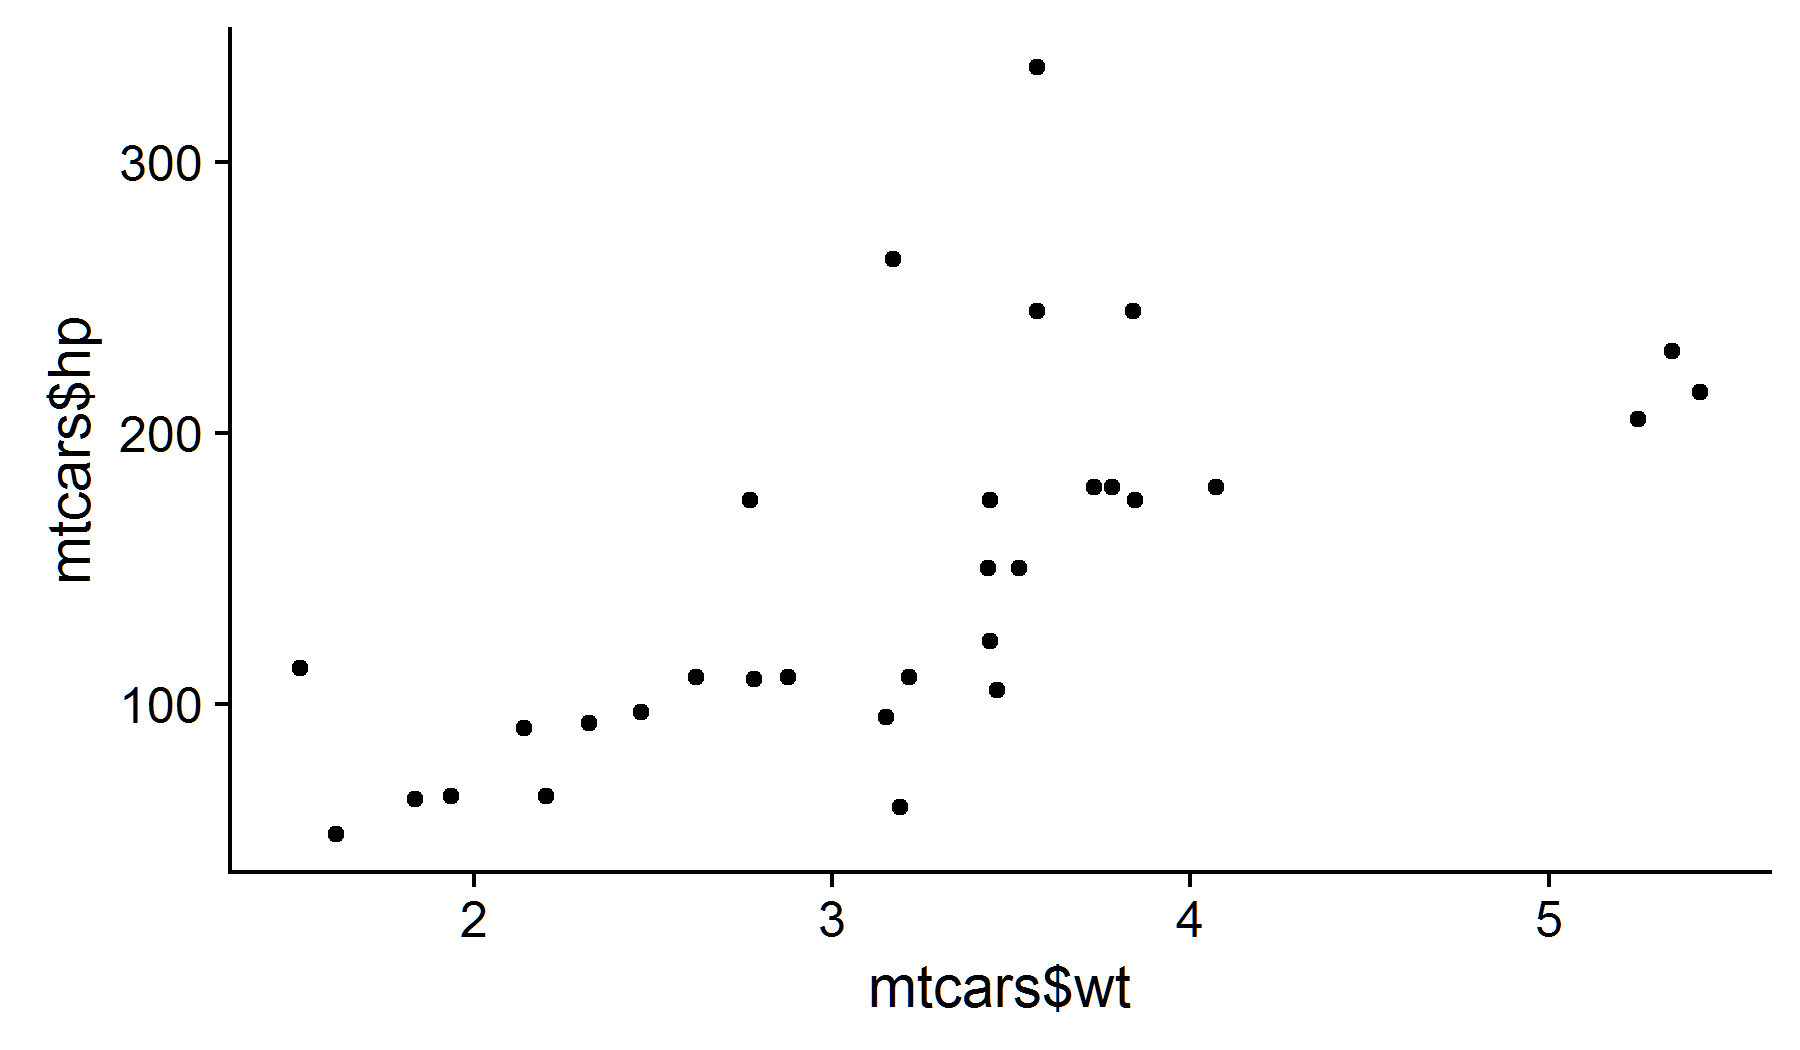
\includegraphics{RIntermediate_files/figure-latex/unnamed-chunk-99-1} \end{adjustwidth}

\begin{Shaded}
\begin{Highlighting}[]

\CommentTok{# Check out the currently attached packages again}
\KeywordTok{search}\NormalTok{()}
\NormalTok{    [}\DecValTok{1}\NormalTok{] }\StringTok{".GlobalEnv"}            \StringTok{"package:BiocStyle"}     \StringTok{"package:cowplot"}      
\NormalTok{    [}\DecValTok{4}\NormalTok{] }\StringTok{"package:forcats"}       \StringTok{"package:stringr"}       \StringTok{"package:dplyr"}        
\NormalTok{    [}\DecValTok{7}\NormalTok{] }\StringTok{"package:purrr"}         \StringTok{"package:readr"}         \StringTok{"package:tidyr"}        
\NormalTok{   [}\DecValTok{10}\NormalTok{] }\StringTok{"package:tibble"}        \StringTok{"package:ggplot2"}       \StringTok{"package:tidyverse"}    
\NormalTok{   [}\DecValTok{13}\NormalTok{] }\StringTok{"package:multtest"}      \StringTok{"package:Biobase"}       \StringTok{"package:BiocGenerics"} 
\NormalTok{   [}\DecValTok{16}\NormalTok{] }\StringTok{"package:parallel"}      \StringTok{"package:openxlsx"}      \StringTok{"package:TeachingDemos"}
\NormalTok{   [}\DecValTok{19}\NormalTok{] }\StringTok{"package:knitr"}         \StringTok{"package:rmarkdown"}     \StringTok{"tools:rstudio"}        
\NormalTok{   [}\DecValTok{22}\NormalTok{] }\StringTok{"package:stats"}         \StringTok{"package:graphics"}      \StringTok{"package:grDevices"}    
\NormalTok{   [}\DecValTok{25}\NormalTok{] }\StringTok{"package:utils"}         \StringTok{"package:datasets"}      \StringTok{"package:methods"}      
\NormalTok{   [}\DecValTok{28}\NormalTok{] }\StringTok{"Autoloads"}             \StringTok{"package:base"}
\end{Highlighting}
\end{Shaded}

Awesome! Notice how \texttt{search()} and \texttt{library()} are closely
interconnected functions.

\textbf{Different ways to load a package}

The \texttt{library()} and \texttt{require()} functions are not very
picky when it comes down to argument types: both \texttt{library(rjson)}
as \texttt{library("rjson")} work perfectly fine for loading a package.

Have a look at some more code chunks that (attempt to) load one or more
packages:

```r \# Chunk 1 library(data.table) require(rjson)

\# Chunk 2 library(``data.table'') require(rjson)

\# Chunk 3 library(data.table) require(rjson, character.only = TRUE)

\# Chunk 4 library(c(``data.table'', ``rjson'')) ```

Select the option that lists all of the chunks that do not generate an
error. The console on the right is yours to experiment in.

\textbf{Instructions}

\begin{verbatim}
   [1] "only chunk1 and chunk2 do not generate errors"
\end{verbatim}

Great! Indeed, only chunk 1 and chunk 2 are correct. Can you figure out
why the last two aren't valid? This exercise concludes the chapter on
functions.

\section{The apply family}\label{the-apply-family}

\subsection{lapply}\label{lapply}

\textbf{Use lapply with a built-in R function}

Before you go about solving the exercises below, have a look at the
documentation of the lapply() function. The Usage section shows the
following expression:

\begin{Shaded}
\begin{Highlighting}[]
\KeywordTok{lapply}\NormalTok{(X, FUN, ...)}
\end{Highlighting}
\end{Shaded}

To put it generally, \texttt{lapply} takes a vector or list \texttt{X},
and applies the function \texttt{FUN} to each of its members. If
\texttt{FUN} requires additional arguments, you pass them after you've
specified \texttt{X} and \texttt{FUN} (\texttt{...}). The output of
\texttt{lapply()} is a list, the same length as \texttt{X}, where each
element is the result of applying \texttt{FUN} on the corresponding
element of \texttt{X}.

Now that you are truly brushing up on your data science skills, let's
revisit some of the most relevant figures in data science history. We've
compiled a vector of famous mathematicians/statisticians and the year
they were born. Up to you to extract some information!

\textbf{Instructions}

\begin{Shaded}
\begin{Highlighting}[]
\OperatorTok{*}\StringTok{ }\NormalTok{Have a look at the }\StringTok{`}\DataTypeTok{strsplit()}\StringTok{`}\NormalTok{ calls, that splits the strings }\ControlFlowTok{in} \StringTok{`}\DataTypeTok{pioneers}\StringTok{`}\NormalTok{ on the }\StringTok{`}\DataTypeTok{:}\StringTok{`}\NormalTok{ sign. The result, }\StringTok{`}\DataTypeTok{split_math}\StringTok{`}\NormalTok{ is a list of }\DecValTok{4}\NormalTok{ character vectors}\OperatorTok{:}\StringTok{ }\NormalTok{the first vector element represents the name, the second element the birth year.}

\OperatorTok{*}\StringTok{ }\NormalTok{Use }\StringTok{`}\DataTypeTok{lapply()}\StringTok{`}\NormalTok{ to convert the character vectors }\ControlFlowTok{in} \StringTok{`}\DataTypeTok{split_math}\StringTok{`}\NormalTok{ to lowercase letters}\OperatorTok{:}\StringTok{ }\NormalTok{apply }\StringTok{`}\DataTypeTok{tolower()}\StringTok{`}\NormalTok{ on each of the elements }\ControlFlowTok{in} \StringTok{`}\DataTypeTok{split_math}\StringTok{`}\NormalTok{. Assign the result, which is a list, to a new variable }\StringTok{`}\DataTypeTok{split_low}\StringTok{`}\NormalTok{.}

\OperatorTok{*}\StringTok{ }\NormalTok{Finally, inspect the contents of }\StringTok{`}\DataTypeTok{split_low}\StringTok{`}\NormalTok{ with }\StringTok{`}\DataTypeTok{str()}\StringTok{`}\NormalTok{.}
\end{Highlighting}
\end{Shaded}

\textbf{Answers}

\begin{Shaded}
\begin{Highlighting}[]
\CommentTok{# The vector pioneers has already been created for you}
\NormalTok{pioneers <-}\StringTok{ }\KeywordTok{c}\NormalTok{(}\StringTok{"GAUSS:1777"}\NormalTok{, }\StringTok{"BAYES:1702"}\NormalTok{, }\StringTok{"PASCAL:1623"}\NormalTok{, }\StringTok{"PEARSON:1857"}\NormalTok{)}

\CommentTok{# Split names from birth year}
\NormalTok{split_math <-}\StringTok{ }\KeywordTok{strsplit}\NormalTok{(pioneers, }\DataTypeTok{split =} \StringTok{":"}\NormalTok{)}

\CommentTok{# Convert to lowercase strings: split_low}
\NormalTok{split_low <-}\StringTok{ }\KeywordTok{lapply}\NormalTok{(split_math, tolower)}

\CommentTok{# Take a look at the structure of split_low}
\KeywordTok{str}\NormalTok{(split_low)}
\NormalTok{   List of }\DecValTok{4}
    \OperatorTok{$}\StringTok{ }\ErrorTok{:}\StringTok{ }\NormalTok{chr [}\DecValTok{1}\OperatorTok{:}\DecValTok{2}\NormalTok{] }\StringTok{"gauss"} \StringTok{"1777"}
    \OperatorTok{$}\StringTok{ }\ErrorTok{:}\StringTok{ }\NormalTok{chr [}\DecValTok{1}\OperatorTok{:}\DecValTok{2}\NormalTok{] }\StringTok{"bayes"} \StringTok{"1702"}
    \OperatorTok{$}\StringTok{ }\ErrorTok{:}\StringTok{ }\NormalTok{chr [}\DecValTok{1}\OperatorTok{:}\DecValTok{2}\NormalTok{] }\StringTok{"pascal"} \StringTok{"1623"}
    \OperatorTok{$}\StringTok{ }\ErrorTok{:}\StringTok{ }\NormalTok{chr [}\DecValTok{1}\OperatorTok{:}\DecValTok{2}\NormalTok{] }\StringTok{"pearson"} \StringTok{"1857"}
\end{Highlighting}
\end{Shaded}

\textbf{Use lapply with your own function}

you can use \texttt{lapply()} on your own functions as well. You just
need to code a new function and make sure it is available in the
workspace. After that, you can use the function inside \texttt{lapply()}
just as you did with base R functions.

In the previous exercise you already used \texttt{lapply()} once to
convert the information about your favorite pioneering statisticians to
a list of vectors composed of two character strings. Let's write some
code to select the names and the birth years separately.

The sample code already includes code that defined
\texttt{select\_first()}, that takes a vector as input and returns the
first element of this vector.

\textbf{Instructions}

\begin{Shaded}
\begin{Highlighting}[]
\OperatorTok{*}\StringTok{ }\NormalTok{Apply }\StringTok{`}\DataTypeTok{select_first()}\StringTok{`}\NormalTok{ over the elements of }\StringTok{`}\DataTypeTok{split_low}\StringTok{`}\NormalTok{ with }\StringTok{`}\DataTypeTok{lapply()}\StringTok{`}\NormalTok{ and assign the result to a new variable }\StringTok{`}\DataTypeTok{names}\StringTok{`}\NormalTok{.}

\OperatorTok{*}\StringTok{ }\NormalTok{Next, write a }\ControlFlowTok{function} \StringTok{`}\DataTypeTok{select_second()}\StringTok{`}\NormalTok{ that does the exact same thing }\ControlFlowTok{for}\NormalTok{ the second element of an inputted vector.}

\OperatorTok{*}\StringTok{ }\NormalTok{Finally, apply the }\StringTok{`}\DataTypeTok{select_second()}\StringTok{`} \ControlFlowTok{function}\NormalTok{ over }\StringTok{`}\DataTypeTok{split_low}\StringTok{`}\NormalTok{ and assign the output to the variable }\StringTok{`}\DataTypeTok{years}\StringTok{`}\NormalTok{.}
\end{Highlighting}
\end{Shaded}

\textbf{Answers}

\begin{Shaded}
\begin{Highlighting}[]
\CommentTok{# Code from previous exercise:}
\NormalTok{pioneers <-}\StringTok{ }\KeywordTok{c}\NormalTok{(}\StringTok{"GAUSS:1777"}\NormalTok{, }\StringTok{"BAYES:1702"}\NormalTok{, }\StringTok{"PASCAL:1623"}\NormalTok{, }\StringTok{"PEARSON:1857"}\NormalTok{)}
\NormalTok{split <-}\StringTok{ }\KeywordTok{strsplit}\NormalTok{(pioneers, }\DataTypeTok{split =} \StringTok{":"}\NormalTok{)}
\NormalTok{split_low <-}\StringTok{ }\KeywordTok{lapply}\NormalTok{(split, tolower)}

\CommentTok{# Write function select_first()}
\NormalTok{select_first <-}\StringTok{ }\ControlFlowTok{function}\NormalTok{(x) \{}
\NormalTok{  x[}\DecValTok{1}\NormalTok{]}
\NormalTok{\}}

\CommentTok{# Apply select_first() over split_low: names}
\NormalTok{names <-}\StringTok{ }\KeywordTok{lapply}\NormalTok{(split_low, select_first)}

\CommentTok{# Write function select_second()}
\NormalTok{select_second <-}\StringTok{ }\ControlFlowTok{function}\NormalTok{(x) \{}
\NormalTok{  x[}\DecValTok{2}\NormalTok{]}
\NormalTok{\}}



\CommentTok{# Apply select_second() over split_low: years}
\NormalTok{years <-}\StringTok{ }\KeywordTok{lapply}\NormalTok{(split_low, select_second)}
\end{Highlighting}
\end{Shaded}

\textbf{lapply and anonymous functions}

Writing your own functions and then using them inside \texttt{lapply()}
is quite an accomplishment! But defining functions to use them only once
is kind of overkill, isn't it? That's why you can use so-called
\textbf{anonymous functions} in R.

Previously, you learned that functions in R are objects in their own
right. This means that they aren't automatically bound to a name. When
you create a function, you can use the assignment operator to give the
function a name. It's perfectly possible, however, to not give the
function a name. This is called an anonymous function:

\begin{Shaded}
\begin{Highlighting}[]
\CommentTok{# Named function}
\NormalTok{triple <-}\StringTok{ }\ControlFlowTok{function}\NormalTok{(x) \{ }\DecValTok{3} \OperatorTok{*}\StringTok{ }\NormalTok{x \}}

\CommentTok{# Anonymous function with same implementation}
\ControlFlowTok{function}\NormalTok{(x) \{ }\DecValTok{3} \OperatorTok{*}\StringTok{ }\NormalTok{x \}}

\CommentTok{# Use anonymous function inside lapply()}
\KeywordTok{lapply}\NormalTok{(}\KeywordTok{list}\NormalTok{(}\DecValTok{1}\NormalTok{,}\DecValTok{2}\NormalTok{,}\DecValTok{3}\NormalTok{), }\ControlFlowTok{function}\NormalTok{(x) \{ }\DecValTok{3} \OperatorTok{*}\StringTok{ }\NormalTok{x \})}
\end{Highlighting}
\end{Shaded}

\textbf{Instructions}

\begin{Shaded}
\begin{Highlighting}[]

\OperatorTok{*}\StringTok{ }\NormalTok{Transform the first call of }\StringTok{`}\DataTypeTok{lapply()}\StringTok{`}\NormalTok{ such that it uses an anonymous }\ControlFlowTok{function}\NormalTok{ that does the same thing.}

\OperatorTok{*}\StringTok{ }\NormalTok{In a similar fashion, convert the second call of }\StringTok{`}\DataTypeTok{lapply}\StringTok{`}\NormalTok{ to use an anonymous version of the }\StringTok{`}\DataTypeTok{select_second()}\StringTok{`}\NormalTok{ function.}

\OperatorTok{*}\StringTok{ }\NormalTok{Remove both the definitions of }\StringTok{`}\DataTypeTok{select_first()}\StringTok{`}\NormalTok{ and }\StringTok{`}\DataTypeTok{select_second()}\StringTok{`}\NormalTok{, as they are no longer useful.}
\end{Highlighting}
\end{Shaded}

\textbf{Answers}

\begin{Shaded}
\begin{Highlighting}[]
\CommentTok{# Definition of split_low}
\NormalTok{pioneers <-}\StringTok{ }\KeywordTok{c}\NormalTok{(}\StringTok{"GAUSS:1777"}\NormalTok{, }\StringTok{"BAYES:1702"}\NormalTok{, }\StringTok{"PASCAL:1623"}\NormalTok{, }\StringTok{"PEARSON:1857"}\NormalTok{)}
\NormalTok{split <-}\StringTok{ }\KeywordTok{strsplit}\NormalTok{(pioneers, }\DataTypeTok{split =} \StringTok{":"}\NormalTok{)}
\NormalTok{split_low <-}\StringTok{ }\KeywordTok{lapply}\NormalTok{(split, tolower)}

\CommentTok{# Transform: use anonymous function inside lapply}
\NormalTok{names <-}\StringTok{ }\KeywordTok{lapply}\NormalTok{(split_low, }\ControlFlowTok{function}\NormalTok{(x) \{ x[}\DecValTok{1}\NormalTok{] \})}

\CommentTok{# Transform: use anonymous function inside lapply}
\NormalTok{years <-}\StringTok{ }\KeywordTok{lapply}\NormalTok{(split_low, }\ControlFlowTok{function}\NormalTok{(x) \{ x[}\DecValTok{2}\NormalTok{] \})}
\end{Highlighting}
\end{Shaded}

Great! Now, there's another way to solve the issue of using the
\texttt{select\_*()} functions only once: you can make a more generic
function that can be used in more places.

\textbf{Use lapply with additional arguments} the \texttt{triple()}
function was transformed to the \texttt{multiply()} function to allow
for a more generic approach. \texttt{lapply()} provides a way to handle
functions that require more than one argument, such as the multiply()
function:

\begin{Shaded}
\begin{Highlighting}[]
\NormalTok{multiply <-}\StringTok{ }\ControlFlowTok{function}\NormalTok{(x, factor) \{}
\NormalTok{  x }\OperatorTok{*}\StringTok{ }\NormalTok{factor}
\NormalTok{\}}
\KeywordTok{lapply}\NormalTok{(}\KeywordTok{list}\NormalTok{(}\DecValTok{1}\NormalTok{,}\DecValTok{2}\NormalTok{,}\DecValTok{3}\NormalTok{), multiply, }\DataTypeTok{factor =} \DecValTok{3}\NormalTok{)}
\end{Highlighting}
\end{Shaded}

On the right we've included a generic version of the select functions
that you've coded earlier: \texttt{select\_el()}. It takes a vector as
its first argument, and an index as its second argument. It returns the
vector's element at the specified index.

\textbf{Instructions}

\begin{Shaded}
\begin{Highlighting}[]
\NormalTok{Use }\StringTok{`}\DataTypeTok{lapply()}\StringTok{`}\NormalTok{ twice to call }\StringTok{`}\DataTypeTok{select_el()}\StringTok{`}\NormalTok{ over all elements }\ControlFlowTok{in} \StringTok{`}\DataTypeTok{split_low}\StringTok{`}\OperatorTok{:}\StringTok{ }\NormalTok{once with the }\StringTok{`}\DataTypeTok{index}\StringTok{`}\NormalTok{ equal to }\DecValTok{1}\NormalTok{ and a second time with the index equal to }\DecValTok{2}\NormalTok{. Assign the result to }\StringTok{`}\DataTypeTok{names}\StringTok{`}\NormalTok{ and }\StringTok{`}\DataTypeTok{years}\StringTok{`}\NormalTok{, respectively.}
\end{Highlighting}
\end{Shaded}

\textbf{Answers}

\begin{Shaded}
\begin{Highlighting}[]
\CommentTok{# Definition of split_low}
\NormalTok{pioneers <-}\StringTok{ }\KeywordTok{c}\NormalTok{(}\StringTok{"GAUSS:1777"}\NormalTok{, }\StringTok{"BAYES:1702"}\NormalTok{, }\StringTok{"PASCAL:1623"}\NormalTok{, }\StringTok{"PEARSON:1857"}\NormalTok{)}
\NormalTok{split <-}\StringTok{ }\KeywordTok{strsplit}\NormalTok{(pioneers, }\DataTypeTok{split =} \StringTok{":"}\NormalTok{)}
\NormalTok{split_low <-}\StringTok{ }\KeywordTok{lapply}\NormalTok{(split, tolower)}

\CommentTok{# Generic select function}
\NormalTok{select_el <-}\StringTok{ }\ControlFlowTok{function}\NormalTok{(x, index) \{}
\NormalTok{  x[index]}
\NormalTok{\}}

\CommentTok{# Use lapply() twice on split_low: names and years}
\NormalTok{names <-}\StringTok{ }\KeywordTok{lapply}\NormalTok{(split_low, select_el, }\DataTypeTok{index =} \DecValTok{1}\NormalTok{)}
\NormalTok{years <-}\StringTok{ }\KeywordTok{lapply}\NormalTok{(split_low, select_el, }\DataTypeTok{index =} \DecValTok{2}\NormalTok{)}
\end{Highlighting}
\end{Shaded}

\textbf{Apply functions that return NULL}

In all of the previous exercises, it was assumed that the functions that
were applied over vectors and lists actually returned a meaningful
result. For example, the \texttt{tolower()} function simply returns the
strings with the characters in lowercase. This won't always be the case.
Suppose you want to display the structure of every element of a list.
You could use the \texttt{str()} function for this, which returns
\texttt{NULL}:

\begin{Shaded}
\begin{Highlighting}[]
\KeywordTok{lapply}\NormalTok{(}\KeywordTok{list}\NormalTok{(}\DecValTok{1}\NormalTok{, }\StringTok{"a"}\NormalTok{, }\OtherTok{TRUE}\NormalTok{), str)}
\end{Highlighting}
\end{Shaded}

This call actually returns a list, the same size as the input list,
containing all \texttt{NULL} values. On the other hand calling

\begin{Shaded}
\begin{Highlighting}[]
\KeywordTok{str}\NormalTok{(}\OtherTok{TRUE}\NormalTok{)}
\end{Highlighting}
\end{Shaded}

on its own prints only the structure of the logical to the console, not
\texttt{NULL}. That's because \texttt{str()} uses \texttt{invisible()}
behind the scenes, which returns an invisible copy of the return value,
\texttt{NULL} in this case. This prevents it from being printed when the
result of \texttt{str()} is not assigned.

What will the following code chunk return (\texttt{split\_low} is
already available in the workspace)? Try to reason about the result
before simply executing it in the console!

\begin{Shaded}
\begin{Highlighting}[]
\KeywordTok{lapply}\NormalTok{(split_low, }\ControlFlowTok{function}\NormalTok{(x) \{}
  \ControlFlowTok{if}\NormalTok{ (}\KeywordTok{nchar}\NormalTok{(x[}\DecValTok{1}\NormalTok{]) }\OperatorTok{>}\StringTok{ }\DecValTok{5}\NormalTok{) \{}
    \KeywordTok{return}\NormalTok{(}\OtherTok{NULL}\NormalTok{)}
\NormalTok{  \} }\ControlFlowTok{else}\NormalTok{ \{}
    \KeywordTok{return}\NormalTok{(x[}\DecValTok{2}\NormalTok{])}
\NormalTok{  \}}
\NormalTok{\})}
\end{Highlighting}
\end{Shaded}

\textbf{Possible Answers}

\begin{Shaded}
\begin{Highlighting}[]
\OperatorTok{*}\StringTok{ `}\DataTypeTok{list(NULL, NULL, "1623", "1857")}\StringTok{`}
\OperatorTok{*}\StringTok{ `}\DataTypeTok{list("gauss", "bayes", NULL, NULL)}\StringTok{`}
\OperatorTok{*}\StringTok{ `}\DataTypeTok{list("1777", "1702", NULL, NULL)}\StringTok{`}
\StringTok{`}\DataTypeTok{ }\StringTok{`}\KeywordTok{list}\NormalTok{(}\StringTok{"1777"}\NormalTok{, }\StringTok{"1702"}\NormalTok{)}\StringTok{`}
\end{Highlighting}
\end{Shaded}

\textbf{Answer}

\begin{verbatim}
   [1] "list(\"1777\", \"1702\", NULL, NULL)"
\end{verbatim}

Wonderful! Feel free to experiment some more with your code in the
console. Did you notice that lapply() always returns a list, no matter
the input? This can be kind of annoying.

\subsection{sapply}\label{sapply}

\textbf{How to use sapply}

You can use \texttt{sapply()} similar to how you used \texttt{lapply()}.
The first argument of \texttt{sapply()} is the list or vector \texttt{X}
over which you want to apply a function, \texttt{FUN}. Potential
additional arguments to this function are specified afterwards
(\texttt{...}):

\begin{Shaded}
\begin{Highlighting}[]
\KeywordTok{sapply}\NormalTok{(X, FUN, ...)}
\end{Highlighting}
\end{Shaded}

In the next couple of exercises, you'll be working with a the variable
\texttt{temp}, that contains temperature measurements for 7 days.
\texttt{temp} is a list of length 7, where each element is a vector of
length 5, representing 5 measurements on a given day. This variable has
already been defined in the workspace: type \texttt{str(temp)} to see
its structure.

\textbf{Instructions}

\begin{Shaded}
\begin{Highlighting}[]
\OperatorTok{*}\StringTok{ }\NormalTok{Use }\StringTok{`}\DataTypeTok{lapply()}\StringTok{`}\NormalTok{ to calculate the }\KeywordTok{minimum}\NormalTok{ (built}\OperatorTok{-}\ControlFlowTok{in} \ControlFlowTok{function} \StringTok{`}\DataTypeTok{min()}\StringTok{`}\NormalTok{) of the temperature measurements }\ControlFlowTok{for}\NormalTok{ every day.}
\OperatorTok{*}\StringTok{ }\NormalTok{Do the same thing but this time with }\StringTok{`}\DataTypeTok{sapply()}\StringTok{`}\NormalTok{. See how the output differs.}
\OperatorTok{*}\StringTok{ }\NormalTok{Use }\StringTok{`}\DataTypeTok{lapply()}\StringTok{`}\NormalTok{ to compute the the }\KeywordTok{maximum}\NormalTok{ (}\StringTok{`}\DataTypeTok{max()}\StringTok{`}\NormalTok{) temperature }\ControlFlowTok{for}\NormalTok{ each day.}
\OperatorTok{*}\StringTok{ }\NormalTok{Again, use }\StringTok{`}\DataTypeTok{sapply()}\StringTok{`}\NormalTok{ to solve the same question and see how }\StringTok{`}\DataTypeTok{lapply()}\StringTok{`}\NormalTok{ and }\StringTok{`}\DataTypeTok{sapply()}\StringTok{`}\NormalTok{ differ.}
\end{Highlighting}
\end{Shaded}

\textbf{Answers}

\begin{Shaded}
\begin{Highlighting}[]
\NormalTok{temp <-}\StringTok{ }\KeywordTok{list}\NormalTok{(}\KeywordTok{c}\NormalTok{(}\DecValTok{3}\NormalTok{,}\DecValTok{7}\NormalTok{,}\DecValTok{9}\NormalTok{,}\DecValTok{6}\NormalTok{,}\OperatorTok{-}\DecValTok{1}\NormalTok{), }\KeywordTok{c}\NormalTok{(}\DecValTok{6}\NormalTok{, }\DecValTok{9}\NormalTok{, }\DecValTok{12}\NormalTok{,}\DecValTok{13}\NormalTok{, }\DecValTok{5}\NormalTok{), }\KeywordTok{c}\NormalTok{(}\DecValTok{4}\NormalTok{, }\DecValTok{8}\NormalTok{, }\DecValTok{3}\NormalTok{, }\OperatorTok{-}\DecValTok{1}\NormalTok{, }\OperatorTok{-}\DecValTok{3}\NormalTok{), }\KeywordTok{c}\NormalTok{(}\DecValTok{1}\NormalTok{, }\DecValTok{4}\NormalTok{, }\DecValTok{7}\NormalTok{, }\DecValTok{2}\NormalTok{, }\OperatorTok{-}\DecValTok{2}\NormalTok{),}
             \KeywordTok{c}\NormalTok{(}\DecValTok{5}\NormalTok{, }\DecValTok{7}\NormalTok{, }\DecValTok{9}\NormalTok{, }\DecValTok{4}\NormalTok{, }\DecValTok{2}\NormalTok{), }\KeywordTok{c}\NormalTok{(}\OperatorTok{-}\DecValTok{3}\NormalTok{, }\DecValTok{5}\NormalTok{, }\DecValTok{8}\NormalTok{, }\DecValTok{9}\NormalTok{, }\DecValTok{4}\NormalTok{), }\KeywordTok{c}\NormalTok{(}\DecValTok{3}\NormalTok{, }\DecValTok{6}\NormalTok{, }\DecValTok{9}\NormalTok{, }\DecValTok{4}\NormalTok{, }\DecValTok{1}\NormalTok{))}

\CommentTok{# temp has already been defined in the workspace}

\CommentTok{# Use lapply() to find each day's minimum temperature}
\KeywordTok{lapply}\NormalTok{(temp, min)}
\NormalTok{   [[}\DecValTok{1}\NormalTok{]]}
\NormalTok{   [}\DecValTok{1}\NormalTok{] }\OperatorTok{-}\DecValTok{1}
   
\NormalTok{   [[}\DecValTok{2}\NormalTok{]]}
\NormalTok{   [}\DecValTok{1}\NormalTok{] }\DecValTok{5}
   
\NormalTok{   [[}\DecValTok{3}\NormalTok{]]}
\NormalTok{   [}\DecValTok{1}\NormalTok{] }\OperatorTok{-}\DecValTok{3}
   
\NormalTok{   [[}\DecValTok{4}\NormalTok{]]}
\NormalTok{   [}\DecValTok{1}\NormalTok{] }\OperatorTok{-}\DecValTok{2}
   
\NormalTok{   [[}\DecValTok{5}\NormalTok{]]}
\NormalTok{   [}\DecValTok{1}\NormalTok{] }\DecValTok{2}
   
\NormalTok{   [[}\DecValTok{6}\NormalTok{]]}
\NormalTok{   [}\DecValTok{1}\NormalTok{] }\OperatorTok{-}\DecValTok{3}
   
\NormalTok{   [[}\DecValTok{7}\NormalTok{]]}
\NormalTok{   [}\DecValTok{1}\NormalTok{] }\DecValTok{1}

\CommentTok{# Use sapply() to find each day's minimum temperature}
\KeywordTok{sapply}\NormalTok{(temp, min)}
\NormalTok{   [}\DecValTok{1}\NormalTok{] }\OperatorTok{-}\DecValTok{1}  \DecValTok{5} \OperatorTok{-}\DecValTok{3} \OperatorTok{-}\DecValTok{2}  \DecValTok{2} \OperatorTok{-}\DecValTok{3}  \DecValTok{1}

\CommentTok{# Use lapply() to find each day's maximum temperature}
\KeywordTok{lapply}\NormalTok{(temp, max)}
\NormalTok{   [[}\DecValTok{1}\NormalTok{]]}
\NormalTok{   [}\DecValTok{1}\NormalTok{] }\DecValTok{9}
   
\NormalTok{   [[}\DecValTok{2}\NormalTok{]]}
\NormalTok{   [}\DecValTok{1}\NormalTok{] }\DecValTok{13}
   
\NormalTok{   [[}\DecValTok{3}\NormalTok{]]}
\NormalTok{   [}\DecValTok{1}\NormalTok{] }\DecValTok{8}
   
\NormalTok{   [[}\DecValTok{4}\NormalTok{]]}
\NormalTok{   [}\DecValTok{1}\NormalTok{] }\DecValTok{7}
   
\NormalTok{   [[}\DecValTok{5}\NormalTok{]]}
\NormalTok{   [}\DecValTok{1}\NormalTok{] }\DecValTok{9}
   
\NormalTok{   [[}\DecValTok{6}\NormalTok{]]}
\NormalTok{   [}\DecValTok{1}\NormalTok{] }\DecValTok{9}
   
\NormalTok{   [[}\DecValTok{7}\NormalTok{]]}
\NormalTok{   [}\DecValTok{1}\NormalTok{] }\DecValTok{9}

\CommentTok{# Use sapply() to find each day's maximum temperature}
\KeywordTok{sapply}\NormalTok{(temp, max)}
\NormalTok{   [}\DecValTok{1}\NormalTok{]  }\DecValTok{9} \DecValTok{13}  \DecValTok{8}  \DecValTok{7}  \DecValTok{9}  \DecValTok{9}  \DecValTok{9}
\end{Highlighting}
\end{Shaded}

Nice! Can you tell the difference between the output of
\texttt{lapply()} and \texttt{sapply()}? The former returns a list,
while the latter returns a vector that is a simplified version of this
list.

\textbf{sapply with your own function}

Like \texttt{lapply()}, \texttt{sapply()} allows you to use self-defined
functions and apply them over a vector or a list:

\begin{Shaded}
\begin{Highlighting}[]
\KeywordTok{sapply}\NormalTok{(X, FUN, ...)}
\end{Highlighting}
\end{Shaded}

Here, \texttt{FUN} can be one of R's built-in functions, but it can also
be a function you wrote. This self-written function can be defined
before hand, or can be inserted directly as an anonymous function.

\textbf{Instructions}

\begin{Shaded}
\begin{Highlighting}[]
\OperatorTok{*}\StringTok{ }\NormalTok{Finish the definition of }\StringTok{`}\DataTypeTok{extremes_avg()}\StringTok{`}\OperatorTok{:}\StringTok{ }\NormalTok{it takes a vector of temperatures and calculates the average of the minimum and maximum temperatures of the vector.}
\OperatorTok{*}\StringTok{ }\NormalTok{Next, use this }\ControlFlowTok{function}\NormalTok{ inside }\StringTok{`}\DataTypeTok{sapply()}\StringTok{`}\NormalTok{ to apply it over the vectors inside }\StringTok{`}\DataTypeTok{temp}\StringTok{`}\NormalTok{.}
\OperatorTok{*}\StringTok{ }\NormalTok{Use the same }\ControlFlowTok{function}\NormalTok{ over }\StringTok{`}\DataTypeTok{temp}\StringTok{`}\NormalTok{ with }\StringTok{`}\DataTypeTok{lapply()}\StringTok{`}\NormalTok{ and see how the outputs differ.}
\end{Highlighting}
\end{Shaded}

\textbf{Answers}

\begin{Shaded}
\begin{Highlighting}[]
\CommentTok{# temp is already defined in the workspace}

\CommentTok{# Finish function definition of extremes_avg}
\NormalTok{extremes_avg <-}\StringTok{ }\ControlFlowTok{function}\NormalTok{(x) \{}
\NormalTok{  ( }\KeywordTok{min}\NormalTok{(x) }\OperatorTok{+}\StringTok{ }\KeywordTok{max}\NormalTok{(x) ) }\OperatorTok{/}\StringTok{ }\DecValTok{2}
\NormalTok{\}}

\CommentTok{# Apply extremes_avg() over temp using sapply()}
\KeywordTok{sapply}\NormalTok{(temp, extremes_avg)}
\NormalTok{   [}\DecValTok{1}\NormalTok{] }\FloatTok{4.0} \FloatTok{9.0} \FloatTok{2.5} \FloatTok{2.5} \FloatTok{5.5} \FloatTok{3.0} \FloatTok{5.0}

\CommentTok{# Apply extremes_avg() over temp using lapply()}
\KeywordTok{lapply}\NormalTok{(temp, extremes_avg)}
\NormalTok{   [[}\DecValTok{1}\NormalTok{]]}
\NormalTok{   [}\DecValTok{1}\NormalTok{] }\DecValTok{4}
   
\NormalTok{   [[}\DecValTok{2}\NormalTok{]]}
\NormalTok{   [}\DecValTok{1}\NormalTok{] }\DecValTok{9}
   
\NormalTok{   [[}\DecValTok{3}\NormalTok{]]}
\NormalTok{   [}\DecValTok{1}\NormalTok{] }\FloatTok{2.5}
   
\NormalTok{   [[}\DecValTok{4}\NormalTok{]]}
\NormalTok{   [}\DecValTok{1}\NormalTok{] }\FloatTok{2.5}
   
\NormalTok{   [[}\DecValTok{5}\NormalTok{]]}
\NormalTok{   [}\DecValTok{1}\NormalTok{] }\FloatTok{5.5}
   
\NormalTok{   [[}\DecValTok{6}\NormalTok{]]}
\NormalTok{   [}\DecValTok{1}\NormalTok{] }\DecValTok{3}
   
\NormalTok{   [[}\DecValTok{7}\NormalTok{]]}
\NormalTok{   [}\DecValTok{1}\NormalTok{] }\DecValTok{5}
\end{Highlighting}
\end{Shaded}

Great job! Of course, you could have solved this exercise using an
anonymous function, but this would require you to use the code inside
the definition of \texttt{extremes\_avg()} twice. Duplicating code
should be avoided as much as possible!

\textbf{sapply with function returning vector}

In the previous exercises, you've seen how \texttt{sapply()} simplifies
the list that \texttt{lapply()} would return by turning it into a
vector. But what if the function you're applying over a list or a vector
returns a vector of length greater than 1? If you don't remember from
the video, don't waste more time in the valley of ignorance and head
over to the instructions!

\textbf{Instructions}

\begin{Shaded}
\begin{Highlighting}[]
\OperatorTok{*}\StringTok{ }\NormalTok{Finish the definition of the }\StringTok{`}\DataTypeTok{extremes()}\StringTok{`}\NormalTok{ function. It takes a vector of numerical values and returns a vector containing the minimum and maximum values of a given vector, with the names }\StringTok{"min"}\NormalTok{ and }\StringTok{"max"}\NormalTok{, respectively.}
\OperatorTok{*}\StringTok{ }\NormalTok{Apply this }\ControlFlowTok{function}\NormalTok{ over the vector }\StringTok{`}\DataTypeTok{temp}\StringTok{`}\NormalTok{ using }\StringTok{`}\DataTypeTok{sapply()}\StringTok{`}\NormalTok{.}
\OperatorTok{*}\StringTok{ }\NormalTok{Finally, apply this }\ControlFlowTok{function}\NormalTok{ over the vector }\StringTok{`}\DataTypeTok{temp}\StringTok{`}\NormalTok{ using }\StringTok{`}\DataTypeTok{lapply()}\StringTok{`}\NormalTok{ as well.}
\end{Highlighting}
\end{Shaded}

\textbf{Answers}

\begin{Shaded}
\begin{Highlighting}[]
\CommentTok{# temp is already available in the workspace}

\CommentTok{# Create a function that returns min and max of a vector: extremes}
\NormalTok{extremes <-}\StringTok{ }\ControlFlowTok{function}\NormalTok{(x) \{}
  \KeywordTok{c}\NormalTok{(}\DataTypeTok{min =} \KeywordTok{min}\NormalTok{(x), }\DataTypeTok{max =} \KeywordTok{max}\NormalTok{(x))}
\NormalTok{\}}

\CommentTok{# Apply extremes() over temp with sapply()}
\KeywordTok{sapply}\NormalTok{(temp, extremes)}
\NormalTok{       [,}\DecValTok{1}\NormalTok{] [,}\DecValTok{2}\NormalTok{] [,}\DecValTok{3}\NormalTok{] [,}\DecValTok{4}\NormalTok{] [,}\DecValTok{5}\NormalTok{] [,}\DecValTok{6}\NormalTok{] [,}\DecValTok{7}\NormalTok{]}
\NormalTok{   min   }\OperatorTok{-}\DecValTok{1}    \DecValTok{5}   \OperatorTok{-}\DecValTok{3}   \OperatorTok{-}\DecValTok{2}    \DecValTok{2}   \OperatorTok{-}\DecValTok{3}    \DecValTok{1}
\NormalTok{   max    }\DecValTok{9}   \DecValTok{13}    \DecValTok{8}    \DecValTok{7}    \DecValTok{9}    \DecValTok{9}    \DecValTok{9}

\CommentTok{# Apply extremes() over temp with lapply()}
\KeywordTok{lapply}\NormalTok{(temp, extremes)}
\NormalTok{   [[}\DecValTok{1}\NormalTok{]]}
\NormalTok{   min max }
    \OperatorTok{-}\DecValTok{1}   \DecValTok{9} 
   
\NormalTok{   [[}\DecValTok{2}\NormalTok{]]}
\NormalTok{   min max }
     \DecValTok{5}  \DecValTok{13} 
   
\NormalTok{   [[}\DecValTok{3}\NormalTok{]]}
\NormalTok{   min max }
    \OperatorTok{-}\DecValTok{3}   \DecValTok{8} 
   
\NormalTok{   [[}\DecValTok{4}\NormalTok{]]}
\NormalTok{   min max }
    \OperatorTok{-}\DecValTok{2}   \DecValTok{7} 
   
\NormalTok{   [[}\DecValTok{5}\NormalTok{]]}
\NormalTok{   min max }
     \DecValTok{2}   \DecValTok{9} 
   
\NormalTok{   [[}\DecValTok{6}\NormalTok{]]}
\NormalTok{   min max }
    \OperatorTok{-}\DecValTok{3}   \DecValTok{9} 
   
\NormalTok{   [[}\DecValTok{7}\NormalTok{]]}
\NormalTok{   min max }
     \DecValTok{1}   \DecValTok{9}
\end{Highlighting}
\end{Shaded}

Wonderful! Have a final look at the console and see how
\texttt{sapply()} did a great job at simplifying the rather
uninformative `list of vectors' that \texttt{lapply()} returns. It
actually returned a nicely formatted matrix!

\textbf{sapply can't simplify, now what?} It seems like we've hit the
jackpot with \texttt{sapply()}. On all of the examples so far,
\texttt{sapply()} was able to nicely simplify the rather bulky output of
\texttt{lapply()}. But, as with life, there are things you can't
simplify. How does \texttt{sapply()} react?

We already created a function, \texttt{below\_zero()}, that takes a
vector of numerical values and returns a vector that only contains the
values that are strictly below zero.

\textbf{Instructions}

\begin{Shaded}
\begin{Highlighting}[]
\OperatorTok{*}\StringTok{ }\NormalTok{Apply }\StringTok{`}\DataTypeTok{below_zero()}\StringTok{`}\NormalTok{ over }\StringTok{`}\DataTypeTok{temp}\StringTok{`}\NormalTok{ using }\StringTok{`}\DataTypeTok{sapply()}\StringTok{`}\NormalTok{ and store the result }\ControlFlowTok{in} \StringTok{`}\DataTypeTok{freezing_s}\StringTok{`}\NormalTok{.}

\OperatorTok{*}\StringTok{ }\NormalTok{Apply }\StringTok{`}\DataTypeTok{below_zero()}\StringTok{`}\NormalTok{ over }\StringTok{`}\DataTypeTok{temp}\StringTok{`}\NormalTok{ using }\StringTok{`}\DataTypeTok{lapply()}\StringTok{`}\NormalTok{. Save the resulting list }\ControlFlowTok{in}\NormalTok{ a variable }\StringTok{`}\DataTypeTok{freezing_l}\StringTok{`}\NormalTok{.}

\OperatorTok{*}\StringTok{ }\NormalTok{Compare }\StringTok{`}\DataTypeTok{freezing_s}\StringTok{`}\NormalTok{ to }\StringTok{`}\DataTypeTok{freezing_l}\StringTok{`}\NormalTok{ using the }\StringTok{`}\DataTypeTok{identical()}\StringTok{`}\NormalTok{ function.}
\end{Highlighting}
\end{Shaded}

\textbf{Answers}

\begin{Shaded}
\begin{Highlighting}[]
\CommentTok{# temp is already prepared for you in the workspace}

\CommentTok{# Definition of below_zero()}
\NormalTok{below_zero <-}\StringTok{ }\ControlFlowTok{function}\NormalTok{(x) \{}
  \KeywordTok{return}\NormalTok{(x[x }\OperatorTok{<}\StringTok{ }\DecValTok{0}\NormalTok{])}
\NormalTok{\}}

\CommentTok{# Apply below_zero over temp using sapply(): freezing_s}
\NormalTok{freezing_s <-}\StringTok{ }\KeywordTok{sapply}\NormalTok{(temp, below_zero)}

\CommentTok{# Apply below_zero over temp using lapply(): freezing_l}
\NormalTok{freezing_l <-}\StringTok{ }\KeywordTok{lapply}\NormalTok{(temp, below_zero)}

\CommentTok{# Are freezing_s and freezing_l identical?}
\KeywordTok{identical}\NormalTok{(freezing_l, freezing_s)}
\NormalTok{   [}\DecValTok{1}\NormalTok{] }\OtherTok{TRUE}
\end{Highlighting}
\end{Shaded}

Nice one! Given that the length of the output of \texttt{below\_zero()}
changes for different input vectors, sapply() is not able to nicely
convert the output of \texttt{lapply()} to a nicely formatted matrix.
Instead, the output values of \texttt{sapply()} and \texttt{lapply()}
are exactly the same, as show by the TRUE output of
\texttt{identical()}.

\textbf{sapply with functions that return NULL}

You already have some apply tricks under your sleeve, but you're surely
hungry for some more, aren't you? In this exercise, you'll see how
\texttt{sapply()} reacts when it is used to apply a function that
returns \texttt{NULL} over a vector or a list.

A function \texttt{print\_info()}, that takes a vector and prints the
average of this vector, has already been created for you. It uses
\texttt{cat()}.

\textbf{Instructions}

\begin{Shaded}
\begin{Highlighting}[]
\OperatorTok{*}\StringTok{ }\NormalTok{Apply }\StringTok{`}\DataTypeTok{print_info()}\StringTok{`}\NormalTok{ over the contents of }\StringTok{`}\DataTypeTok{temp}\StringTok{`}\NormalTok{ with }\StringTok{`}\DataTypeTok{sapply()}\StringTok{`}\NormalTok{.}

\OperatorTok{*}\StringTok{ }\NormalTok{Repeat this process with }\StringTok{`}\DataTypeTok{lapply()}\StringTok{`}\NormalTok{. Do you notice the difference?}
\end{Highlighting}
\end{Shaded}

\textbf{Answers}

\begin{Shaded}
\begin{Highlighting}[]
\CommentTok{# temp is already available in the workspace}

\CommentTok{# Definition of print_info()}
\NormalTok{print_info <-}\StringTok{ }\ControlFlowTok{function}\NormalTok{(x) \{}
  \KeywordTok{cat}\NormalTok{(}\StringTok{"The average temperature is"}\NormalTok{, }\KeywordTok{mean}\NormalTok{(x), }\StringTok{"}\CharTok{\textbackslash{}n}\StringTok{"}\NormalTok{)}
\NormalTok{\}}

\CommentTok{# Apply print_info() over temp using sapply()}
\KeywordTok{sapply}\NormalTok{(temp, print_info)}
\NormalTok{   The average temperature is }\FloatTok{4.8} 
\NormalTok{   The average temperature is }\DecValTok{9} 
\NormalTok{   The average temperature is }\FloatTok{2.2} 
\NormalTok{   The average temperature is }\FloatTok{2.4} 
\NormalTok{   The average temperature is }\FloatTok{5.4} 
\NormalTok{   The average temperature is }\FloatTok{4.6} 
\NormalTok{   The average temperature is }\FloatTok{4.6}
\NormalTok{   [[}\DecValTok{1}\NormalTok{]]}
   \OtherTok{NULL}
   
\NormalTok{   [[}\DecValTok{2}\NormalTok{]]}
   \OtherTok{NULL}
   
\NormalTok{   [[}\DecValTok{3}\NormalTok{]]}
   \OtherTok{NULL}
   
\NormalTok{   [[}\DecValTok{4}\NormalTok{]]}
   \OtherTok{NULL}
   
\NormalTok{   [[}\DecValTok{5}\NormalTok{]]}
   \OtherTok{NULL}
   
\NormalTok{   [[}\DecValTok{6}\NormalTok{]]}
   \OtherTok{NULL}
   
\NormalTok{   [[}\DecValTok{7}\NormalTok{]]}
   \OtherTok{NULL}

\CommentTok{# Apply print_info() over temp using lapply()}
\KeywordTok{lapply}\NormalTok{(temp, print_info)}
\NormalTok{   The average temperature is }\FloatTok{4.8} 
\NormalTok{   The average temperature is }\DecValTok{9} 
\NormalTok{   The average temperature is }\FloatTok{2.2} 
\NormalTok{   The average temperature is }\FloatTok{2.4} 
\NormalTok{   The average temperature is }\FloatTok{5.4} 
\NormalTok{   The average temperature is }\FloatTok{4.6} 
\NormalTok{   The average temperature is }\FloatTok{4.6}
\NormalTok{   [[}\DecValTok{1}\NormalTok{]]}
   \OtherTok{NULL}
   
\NormalTok{   [[}\DecValTok{2}\NormalTok{]]}
   \OtherTok{NULL}
   
\NormalTok{   [[}\DecValTok{3}\NormalTok{]]}
   \OtherTok{NULL}
   
\NormalTok{   [[}\DecValTok{4}\NormalTok{]]}
   \OtherTok{NULL}
   
\NormalTok{   [[}\DecValTok{5}\NormalTok{]]}
   \OtherTok{NULL}
   
\NormalTok{   [[}\DecValTok{6}\NormalTok{]]}
   \OtherTok{NULL}
   
\NormalTok{   [[}\DecValTok{7}\NormalTok{]]}
   \OtherTok{NULL}
\end{Highlighting}
\end{Shaded}

Great! Notice here that, quite surprisingly, \texttt{sapply()} does not
simplify the list of \texttt{NULL\textquotesingle{}s}. That's because
the `vector-version' of a list of \texttt{NULL\textquotesingle{}s} would
simply be a \texttt{NULL}, which is no longer a vector with the same
length as the input.

\textbf{Reverse engineering sapply}

\begin{Shaded}
\begin{Highlighting}[]
\KeywordTok{sapply}\NormalTok{(}\KeywordTok{list}\NormalTok{(}\KeywordTok{runif}\NormalTok{ (}\DecValTok{10}\NormalTok{), }\KeywordTok{runif}\NormalTok{ (}\DecValTok{10}\NormalTok{)), }
       \ControlFlowTok{function}\NormalTok{(x) }\KeywordTok{c}\NormalTok{(}\DataTypeTok{min =} \KeywordTok{min}\NormalTok{(x), }\DataTypeTok{mean =} \KeywordTok{mean}\NormalTok{(x), }\DataTypeTok{max =} \KeywordTok{max}\NormalTok{(x)))}
\end{Highlighting}
\end{Shaded}

Without going straight to the console to run the code, try to reason
which of the following statements are correct and why.

\begin{enumerate}
\def\labelenumi{(\arabic{enumi})}
\tightlist
\item
  \texttt{sapply()} can't simplify the result that \texttt{lapply()}
  would return, and thus returns a list of vectors.
\item
  This code generates a matrix with 3 rows and 2 columns.
\item
  The function that is used inside \texttt{sapply()} is anonymous.
\item
  The resulting data structure does not contain any names.
\end{enumerate}

Select the option that lists all correct statements.

\textbf{Possible Answers}

\begin{Shaded}
\begin{Highlighting}[]
\OperatorTok{*}\StringTok{ }\NormalTok{(}\DecValTok{1}\NormalTok{) }\KeywordTok{and}\NormalTok{ (}\DecValTok{3}\NormalTok{)}
\OperatorTok{*}\StringTok{ }\NormalTok{(}\DecValTok{2}\NormalTok{) }\KeywordTok{and}\NormalTok{ (}\DecValTok{3}\NormalTok{)}
\OperatorTok{*}\StringTok{ }\NormalTok{(}\DecValTok{1}\NormalTok{) }\KeywordTok{and}\NormalTok{ (}\DecValTok{4}\NormalTok{)}
\OperatorTok{*}\StringTok{ }\NormalTok{(}\DecValTok{2}\NormalTok{), (}\DecValTok{3}\NormalTok{) }\KeywordTok{and}\NormalTok{ (}\DecValTok{4}\NormalTok{)}
\end{Highlighting}
\end{Shaded}

\textbf{Answer}

\begin{verbatim}
   [1] "(2) and (3)"
\end{verbatim}

Great! This concludes the exercise set on sapply()

\subsection{vapply}\label{vapply}

\textbf{Use vapply} Before you get your hands dirty with the third and
last apply function that you'll learn about in this intermediate R
course, let's take a look at its syntax. The function is called
\texttt{vapply()}, and it has the following syntax:

\begin{Shaded}
\begin{Highlighting}[]
\KeywordTok{vapply}\NormalTok{(X, FUN, FUN.VALUE, ..., }\DataTypeTok{USE.NAMES =} \OtherTok{TRUE}\NormalTok{)}
\end{Highlighting}
\end{Shaded}

Over the elements inside \texttt{X}, the function \texttt{FUN} is
applied. The \texttt{FUN.VALUE} argument expects a template for the
return argument of this function \texttt{FUN}. \texttt{USE.NAMES} is
\texttt{TRUE} by default; in this case \texttt{vapply()} tries to
generate a named array, if possible.

For the next set of exercises, you'll be working on the \texttt{temp}
list again, that contains 7 numerical vectors of length 5. We also coded
a function \texttt{basics()} that takes a vector, and returns a named
vector of length three, containing the minimum, mean and maximum value
of the vector respectively.

\textbf{Instruction}

\begin{Shaded}
\begin{Highlighting}[]
\OperatorTok{*}\StringTok{ }\NormalTok{Apply the }\ControlFlowTok{function} \StringTok{`}\DataTypeTok{basics()}\StringTok{`}\NormalTok{ over the list of temperatures, }\StringTok{`}\DataTypeTok{temp}\StringTok{`}\NormalTok{, using }\StringTok{`}\DataTypeTok{vapply()}\StringTok{`}\NormalTok{. This time,   you can use }\StringTok{`}\DataTypeTok{numeric(3)}\StringTok{`}\NormalTok{ to specify the }\StringTok{`}\DataTypeTok{FUN.VALUE}\StringTok{`}\NormalTok{ argument.}
\end{Highlighting}
\end{Shaded}

\textbf{Answers}

\begin{Shaded}
\begin{Highlighting}[]
\CommentTok{# temp is already available in the workspace}

\CommentTok{# Definition of basics()}
\NormalTok{basics <-}\StringTok{ }\ControlFlowTok{function}\NormalTok{(x) \{}
  \KeywordTok{c}\NormalTok{(}\DataTypeTok{min =} \KeywordTok{min}\NormalTok{(x), }\DataTypeTok{mean =} \KeywordTok{mean}\NormalTok{(x), }\DataTypeTok{max =} \KeywordTok{max}\NormalTok{(x))}
\NormalTok{\}}

\CommentTok{# Apply basics() over temp using vapply()}
\KeywordTok{vapply}\NormalTok{(temp, basics, }\KeywordTok{numeric}\NormalTok{(}\DecValTok{3}\NormalTok{))}
\NormalTok{        [,}\DecValTok{1}\NormalTok{] [,}\DecValTok{2}\NormalTok{] [,}\DecValTok{3}\NormalTok{] [,}\DecValTok{4}\NormalTok{] [,}\DecValTok{5}\NormalTok{] [,}\DecValTok{6}\NormalTok{] [,}\DecValTok{7}\NormalTok{]}
\NormalTok{   min  }\OperatorTok{-}\FloatTok{1.0}    \DecValTok{5} \OperatorTok{-}\FloatTok{3.0} \OperatorTok{-}\FloatTok{2.0}  \FloatTok{2.0} \OperatorTok{-}\FloatTok{3.0}  \FloatTok{1.0}
\NormalTok{   mean  }\FloatTok{4.8}    \DecValTok{9}  \FloatTok{2.2}  \FloatTok{2.4}  \FloatTok{5.4}  \FloatTok{4.6}  \FloatTok{4.6}
\NormalTok{   max   }\FloatTok{9.0}   \DecValTok{13}  \FloatTok{8.0}  \FloatTok{7.0}  \FloatTok{9.0}  \FloatTok{9.0}  \FloatTok{9.0}
\end{Highlighting}
\end{Shaded}

Perfect! Notice how, just as with \texttt{sapply()}, \texttt{vapply()}
neatly transfers the names that you specify in the \texttt{basics()}
function to the row names of the matrix that it returns.

\textbf{Use vapply (2)}

So far you've seen that \texttt{vapply()} mimics the behavior of
\texttt{sapply()} if everything goes according to plan. But what if it
doesn't?

there are cases where the structure of the output of the function you
want to apply, \texttt{FUN}, does not correspond to the template you
specify in \texttt{FUN.VALUE}. In that case, \texttt{vapply()} will
throw an error that informs you about the misalignment between expected
and actual output.

\textbf{Instructions}

\begin{Shaded}
\begin{Highlighting}[]
\OperatorTok{*}\StringTok{ }\NormalTok{Inspect the code on the right and try to run it. If you haven}\StringTok{'t changed anything, an error should pop up. That'}\NormalTok{s because }\StringTok{`}\DataTypeTok{vapply()}\StringTok{`}\NormalTok{ still expects }\StringTok{`}\DataTypeTok{basics()}\StringTok{`}\NormalTok{ to return a vector of length }\DecValTok{3}\NormalTok{. The error message gives you an indication of what}\StringTok{'s wrong.}

\StringTok{* Try to fix the error by editing the `vapply()` command.}
\end{Highlighting}
\end{Shaded}

\textbf{Answers}

\begin{Shaded}
\begin{Highlighting}[]
\CommentTok{# temp is already available in the workspace}

\CommentTok{# Definition of the basics() function}
\NormalTok{basics <-}\StringTok{ }\ControlFlowTok{function}\NormalTok{(x) \{}
  \KeywordTok{c}\NormalTok{(}\DataTypeTok{min =} \KeywordTok{min}\NormalTok{(x), }\DataTypeTok{mean =} \KeywordTok{mean}\NormalTok{(x), }\DataTypeTok{median =} \KeywordTok{median}\NormalTok{(x), }\DataTypeTok{max =} \KeywordTok{max}\NormalTok{(x))}
\NormalTok{\}}

\CommentTok{# Fix the error:}
\KeywordTok{vapply}\NormalTok{(temp, basics, }\KeywordTok{numeric}\NormalTok{(}\DecValTok{4}\NormalTok{))}
\NormalTok{          [,}\DecValTok{1}\NormalTok{] [,}\DecValTok{2}\NormalTok{] [,}\DecValTok{3}\NormalTok{] [,}\DecValTok{4}\NormalTok{] [,}\DecValTok{5}\NormalTok{] [,}\DecValTok{6}\NormalTok{] [,}\DecValTok{7}\NormalTok{]}
\NormalTok{   min    }\OperatorTok{-}\FloatTok{1.0}    \DecValTok{5} \OperatorTok{-}\FloatTok{3.0} \OperatorTok{-}\FloatTok{2.0}  \FloatTok{2.0} \OperatorTok{-}\FloatTok{3.0}  \FloatTok{1.0}
\NormalTok{   mean    }\FloatTok{4.8}    \DecValTok{9}  \FloatTok{2.2}  \FloatTok{2.4}  \FloatTok{5.4}  \FloatTok{4.6}  \FloatTok{4.6}
\NormalTok{   median  }\FloatTok{6.0}    \DecValTok{9}  \FloatTok{3.0}  \FloatTok{2.0}  \FloatTok{5.0}  \FloatTok{5.0}  \FloatTok{4.0}
\NormalTok{   max     }\FloatTok{9.0}   \DecValTok{13}  \FloatTok{8.0}  \FloatTok{7.0}  \FloatTok{9.0}  \FloatTok{9.0}  \FloatTok{9.0}
\end{Highlighting}
\end{Shaded}

\textbf{From sapply to vapply}

As highlighted before, \texttt{vapply()} can be considered a more robust
version of \texttt{sapply()}, because you explicitly restrict the output
of the function you want to apply. Converting your \texttt{sapply()}
expressions in your own R scripts to \texttt{vapply()} expressions is
therefore a good practice (and also a breeze!).

\textbf{Instructions}

\begin{Shaded}
\begin{Highlighting}[]
\NormalTok{Convert all the }\StringTok{`}\DataTypeTok{sapply()}\StringTok{`}\NormalTok{ expressions on the right to their }\StringTok{`}\DataTypeTok{vapply()}\StringTok{`}\NormalTok{ counterparts. Their results should be exactly the same; you}\StringTok{'re only adding robustness. You'}\NormalTok{ll need the templates }\StringTok{`}\DataTypeTok{numeric(1)}\StringTok{`}\NormalTok{ and }\StringTok{`}\DataTypeTok{logical(1)}\StringTok{`}\NormalTok{.}
\end{Highlighting}
\end{Shaded}

\textbf{Answers}

\begin{Shaded}
\begin{Highlighting}[]
\CommentTok{# temp is already defined in the workspace}

\CommentTok{# Convert to vapply() expression}
\KeywordTok{vapply}\NormalTok{(temp, max, }\KeywordTok{numeric}\NormalTok{(}\DecValTok{1}\NormalTok{))}
\NormalTok{   [}\DecValTok{1}\NormalTok{]  }\DecValTok{9} \DecValTok{13}  \DecValTok{8}  \DecValTok{7}  \DecValTok{9}  \DecValTok{9}  \DecValTok{9}

\CommentTok{# Convert to vapply() expression}
\KeywordTok{vapply}\NormalTok{(temp, }\ControlFlowTok{function}\NormalTok{(x, y) \{ }\KeywordTok{mean}\NormalTok{(x) }\OperatorTok{>}\StringTok{ }\NormalTok{y \}, }\KeywordTok{logical}\NormalTok{(}\DecValTok{1}\NormalTok{), }\DataTypeTok{y =} \DecValTok{5}\NormalTok{)}
\NormalTok{   [}\DecValTok{1}\NormalTok{] }\OtherTok{FALSE}  \OtherTok{TRUE} \OtherTok{FALSE} \OtherTok{FALSE}  \OtherTok{TRUE} \OtherTok{FALSE} \OtherTok{FALSE}
\end{Highlighting}
\end{Shaded}

\textbf{Mathematical utilities}

Have another look at some useful math functions that R features:

\begin{itemize}
\tightlist
\item
  \texttt{abs()}: calculate the absolute value.
\item
  \texttt{sum()}: calculate the sum of all the values in a data
  structure.
\item
  \texttt{mean()}: calculate the arithmetic mean.
\item
  \texttt{round()}: Round the values to 0 decimal places by default. Try
  out \texttt{?round} in the console for variations of \texttt{round()}
  and ways to change the number of digits to round to.
\end{itemize}

As a data scientst in training, you've estimated a regression model on
the sales data for the past six months. After evaluating your model, you
see that the training error of your model is quite regular, showing both
positive and negative values. The error values are already defined in
the workspace on the right (\texttt{errors}).

\textbf{Instructions}

\begin{Shaded}
\begin{Highlighting}[]
\NormalTok{Calculate the sum of the absolute rounded values of the training errors. You can work }\ControlFlowTok{in}\NormalTok{ parts, or with a single one}\OperatorTok{-}\NormalTok{liner. There}\StringTok{'s no need to store the result in a variable, just have R print it.}
\end{Highlighting}
\end{Shaded}

\textbf{Answers}

\begin{Shaded}
\begin{Highlighting}[]
\CommentTok{# The errors vector has already been defined for you}
\NormalTok{errors <-}\StringTok{ }\KeywordTok{c}\NormalTok{(}\FloatTok{1.9}\NormalTok{, }\OperatorTok{-}\FloatTok{2.6}\NormalTok{, }\FloatTok{4.0}\NormalTok{, }\OperatorTok{-}\FloatTok{9.5}\NormalTok{, }\OperatorTok{-}\FloatTok{3.4}\NormalTok{, }\FloatTok{7.3}\NormalTok{)}

\CommentTok{# Sum of absolute rounded values of errors}
\KeywordTok{sum}\NormalTok{(}\KeywordTok{round}\NormalTok{(}\KeywordTok{abs}\NormalTok{(errors)))}
\NormalTok{   [}\DecValTok{1}\NormalTok{] }\DecValTok{29}
\end{Highlighting}
\end{Shaded}

\textbf{Find the error}

We went ahead and included some code on the right, but there's still an
error. Can you trace it and fix it?

In times of despair, help with functions such as \texttt{sum()} and
\texttt{rev()} are a single command away; simply use \texttt{?sum} and
\texttt{?rev} in the console.

\textbf{Instructions}

\begin{Shaded}
\begin{Highlighting}[]
\NormalTok{Fix the error by including code on the last line. Remember}\OperatorTok{:}\StringTok{ }\NormalTok{you want to call }\StringTok{`}\DataTypeTok{mean()}\StringTok{`}\NormalTok{ only once}\OperatorTok{!}
\end{Highlighting}
\end{Shaded}

\textbf{Answers}

\begin{Shaded}
\begin{Highlighting}[]
\CommentTok{# Don't edit these two lines}
\NormalTok{vec1 <-}\StringTok{ }\KeywordTok{c}\NormalTok{(}\FloatTok{1.5}\NormalTok{, }\FloatTok{2.5}\NormalTok{, }\FloatTok{8.4}\NormalTok{, }\FloatTok{3.7}\NormalTok{, }\FloatTok{6.3}\NormalTok{)}
\NormalTok{vec2 <-}\StringTok{ }\KeywordTok{rev}\NormalTok{(vec1)}

\CommentTok{# Fix the error}
\KeywordTok{mean}\NormalTok{(}\KeywordTok{append}\NormalTok{(}\KeywordTok{abs}\NormalTok{(vec1), }\KeywordTok{abs}\NormalTok{(vec2)))}
\NormalTok{   [}\DecValTok{1}\NormalTok{] }\FloatTok{4.48}
\end{Highlighting}
\end{Shaded}

Nice work! If you check out the documentation of \texttt{mean()}, you'll
see that only the first argument, \texttt{x}, should be a vector. If you
also specify a second argument, R will match the arguments by position
and expect a specification of the \texttt{trim} argument. Therefore,
merging the two vectors is a must!

\textbf{Data Utilities}

R features a bunch of functions to juggle around with data structures::

\emph{\texttt{seq()}: Generate sequences, by specifying the
\texttt{from}, \texttt{to} and \texttt{by} arguments. }\texttt{rep()}:
Replicate elements of vectors and lists. \emph{\texttt{sort()}: Sort a
vector in ascending order. Works on numerics, but also on character
strings and logicals. }\texttt{rev()}: Reverse the elements in a data
structures for which reversal is defined. \emph{\texttt{str()}: Display
the structure of any R object. }\texttt{append()}: Merge vectors or
lists. \emph{\texttt{is.*()}: Check for the class of an R object.
}\texttt{as.*()}: Convert an R object from one class to another.
*\texttt{unlist()}: Flatten (possibly embedded) lists to produce a
vector.

Remember the social media profile view data? Your LinkedIn and Facebook
view counts for the last seven days are already defined as lists on the
right.

\textbf{Instructions}

\begin{Shaded}
\begin{Highlighting}[]
\OperatorTok{*}\StringTok{ }\NormalTok{Convert both }\StringTok{`}\DataTypeTok{linkedin}\StringTok{`}\NormalTok{ and }\StringTok{`}\DataTypeTok{facebook}\StringTok{`}\NormalTok{ lists to a vector, and store them as }\StringTok{`}\DataTypeTok{li_vec}\StringTok{`}\NormalTok{ and }\StringTok{`}\DataTypeTok{fb_vec}\StringTok{`}\NormalTok{ respectively.}

\OperatorTok{*}\NormalTok{Next, append }\StringTok{`}\DataTypeTok{fb_vec}\StringTok{`}\NormalTok{ to the }\StringTok{`}\DataTypeTok{li_vec}\StringTok{`}\NormalTok{ (Facebook data comes last). Save the result as }\StringTok{`}\DataTypeTok{social_vec}\StringTok{`}\NormalTok{.}

\OperatorTok{*}\NormalTok{Finally, sort }\StringTok{`}\DataTypeTok{social_vec}\StringTok{`}\NormalTok{ from high to low. Print the resulting vector.}
\end{Highlighting}
\end{Shaded}

\textbf{Answers}

\begin{Shaded}
\begin{Highlighting}[]
\CommentTok{# The linkedin and facebook lists have already been created for you}
\NormalTok{linkedin <-}\StringTok{ }\KeywordTok{list}\NormalTok{(}\DecValTok{16}\NormalTok{, }\DecValTok{9}\NormalTok{, }\DecValTok{13}\NormalTok{, }\DecValTok{5}\NormalTok{, }\DecValTok{2}\NormalTok{, }\DecValTok{17}\NormalTok{, }\DecValTok{14}\NormalTok{)}
\NormalTok{facebook <-}\StringTok{ }\KeywordTok{list}\NormalTok{(}\DecValTok{17}\NormalTok{, }\DecValTok{7}\NormalTok{, }\DecValTok{5}\NormalTok{, }\DecValTok{16}\NormalTok{, }\DecValTok{8}\NormalTok{, }\DecValTok{13}\NormalTok{, }\DecValTok{14}\NormalTok{)}

\CommentTok{# Convert linkedin and facebook to a vector: li_vec and fb_vec}
\NormalTok{li_vec <-}\StringTok{ }\KeywordTok{unlist}\NormalTok{(linkedin)}
\NormalTok{fb_vec <-}\StringTok{ }\KeywordTok{unlist}\NormalTok{(facebook)}

\CommentTok{# Append fb_vec to li_vec: social_vec}
\NormalTok{social_vec <-}\StringTok{ }\KeywordTok{append}\NormalTok{(li_vec, fb_vec)}

\CommentTok{# Sort social_vec}
\KeywordTok{sort}\NormalTok{(social_vec, }\DataTypeTok{decreasing =} \OtherTok{TRUE}\NormalTok{)}
\NormalTok{    [}\DecValTok{1}\NormalTok{] }\DecValTok{17} \DecValTok{17} \DecValTok{16} \DecValTok{16} \DecValTok{14} \DecValTok{14} \DecValTok{13} \DecValTok{13}  \DecValTok{9}  \DecValTok{8}  \DecValTok{7}  \DecValTok{5}  \DecValTok{5}  \DecValTok{2}
\end{Highlighting}
\end{Shaded}

Wonderful! These instructions required you to solve this challenge in a
step-by-step approach. If you're comfortable with the functions, you can
combine some of these steps into powerful one-liners.

\textbf{Find the error (2)}

Just as before, let's switch roles. It's up to you to see what
unforgivable mistakes we've made. Go fix them!

\textbf{Instructions}

\begin{Shaded}
\begin{Highlighting}[]
\NormalTok{Correct the expression. Make sure that your fix still uses the functions }\StringTok{`}\DataTypeTok{rep()}\StringTok{`}\NormalTok{ and }\StringTok{`}\DataTypeTok{seq()}\StringTok{`}\NormalTok{.}
\end{Highlighting}
\end{Shaded}

\textbf{Answers}

\begin{Shaded}
\begin{Highlighting}[]
\CommentTok{# Fix me}
\CommentTok{# seq(rep(1, 7, by = 2), times = 7)}
\KeywordTok{rep}\NormalTok{(}\KeywordTok{seq}\NormalTok{(}\DecValTok{1}\NormalTok{, }\DecValTok{7}\NormalTok{, }\DataTypeTok{by =} \DecValTok{2}\NormalTok{), }\DataTypeTok{times =} \DecValTok{7}\NormalTok{)}
\NormalTok{    [}\DecValTok{1}\NormalTok{] }\DecValTok{1} \DecValTok{3} \DecValTok{5} \DecValTok{7} \DecValTok{1} \DecValTok{3} \DecValTok{5} \DecValTok{7} \DecValTok{1} \DecValTok{3} \DecValTok{5} \DecValTok{7} \DecValTok{1} \DecValTok{3} \DecValTok{5} \DecValTok{7} \DecValTok{1} \DecValTok{3} \DecValTok{5} \DecValTok{7} \DecValTok{1} \DecValTok{3} \DecValTok{5} \DecValTok{7} \DecValTok{1} \DecValTok{3} \DecValTok{5} \DecValTok{7}
\end{Highlighting}
\end{Shaded}

Wonderful! Debugging code is also a big part of the daily routine of a
data scientist, and you seem to be great at it!

\textbf{Beat Gauss using R}

There is a popular story about young Gauss. As a pupil, he had a lazy
teacher who wanted to keep the classroom busy by having them add up the
numbers 1 to 100. Gauss came up with an answer almost instantaneously,
5050. On the spot, he had developed a formula for calculating the sum of
an arithmetic series. There are more general formulas for calculating
the sum of an arithmetic series with different starting values and
increments. Instead of deriving such a formula, why not use R to
calculate the sum of a sequence?

\textbf{Instructions}

\begin{Shaded}
\begin{Highlighting}[]

\OperatorTok{*}\StringTok{ }\NormalTok{Using the }\ControlFlowTok{function} \StringTok{`}\DataTypeTok{seq()}\StringTok{`}\NormalTok{, create a sequence that ranges from }\DecValTok{1}\NormalTok{ to }\DecValTok{500} \ControlFlowTok{in}\NormalTok{ increments of }\DecValTok{3}\NormalTok{. Assign the resulting vector to a variable }\StringTok{`}\DataTypeTok{seq1}\StringTok{`}\NormalTok{.}

\OperatorTok{*}\StringTok{ }\NormalTok{Again with the }\ControlFlowTok{function} \StringTok{`}\DataTypeTok{seq()}\StringTok{`}\NormalTok{, create a sequence that ranges from }\DecValTok{1200}\NormalTok{ to }\DecValTok{900} \ControlFlowTok{in}\NormalTok{ increments of }\OperatorTok{-}\DecValTok{7}\NormalTok{. Assign it to a variable }\StringTok{`}\DataTypeTok{seq2}\StringTok{`}\NormalTok{.}

\OperatorTok{*}\StringTok{ }\NormalTok{Calculate the total sum of the sequences, either by using the }\StringTok{`}\DataTypeTok{sum()}\StringTok{`} \ControlFlowTok{function}\NormalTok{ twice and adding the two results, or by first concatenating the sequences and then using the }\StringTok{`}\DataTypeTok{sum()}\StringTok{`} \ControlFlowTok{function}\NormalTok{ once. Print the result to the console.}
\end{Highlighting}
\end{Shaded}

\textbf{Answers}

\begin{Shaded}
\begin{Highlighting}[]
\CommentTok{# Create first sequence: seq1}
\NormalTok{seq1 <-}\StringTok{ }\KeywordTok{seq}\NormalTok{(}\DecValTok{1}\NormalTok{, }\DecValTok{500}\NormalTok{, }\DataTypeTok{by =} \DecValTok{3}\NormalTok{)}

\CommentTok{# Create second sequence: seq2}
\NormalTok{seq2 <-}\StringTok{ }\KeywordTok{seq}\NormalTok{(}\DecValTok{1200}\NormalTok{, }\DecValTok{900}\NormalTok{, }\DataTypeTok{by =} \OperatorTok{-}\DecValTok{7}\NormalTok{)}

\CommentTok{# Calculate total sum of the sequences}
\KeywordTok{sum}\NormalTok{(seq1) }\OperatorTok{+}\StringTok{ }\KeywordTok{sum}\NormalTok{(seq2)}
\NormalTok{   [}\DecValTok{1}\NormalTok{] }\DecValTok{87029}
\end{Highlighting}
\end{Shaded}

\section{Utilities}\label{utilities}

\subsection{regular Expressions}\label{regular-expressions}

\textbf{grepl \& grep}

In their most basic form, regular expressions can be used to see whether
a pattern exists inside a character string or a vector of character
strings. For this purpose, you can use:

\begin{itemize}
\item
  \texttt{grepl()}, which returns \texttt{TRUE} when a pattern is found
  in the corresponding character string.
\item
  \texttt{grep()}, which returns a vector of indices of the character
  strings that contains the pattern. Both functions need a
  \texttt{pattern} and \texttt{x} argument, where \texttt{pattern} is
  the regular expression you want to match for, and the \texttt{x}
  argument is the character vector from which matches should be sought.
\end{itemize}

In this and the following exercises, you'll be querying and manipulating
a character vector of email addresses! The vector \texttt{emails} has
already been defined in the editor on the right so you can begin with
the instructions straight away!

\textbf{Instructions}

\begin{Shaded}
\begin{Highlighting}[]
\OperatorTok{*}\StringTok{ }\NormalTok{Use }\StringTok{`}\DataTypeTok{grepl()}\StringTok{`}\NormalTok{ to generate a vector of logicals that indicates whether these email addressess contain }\StringTok{`}\DataTypeTok{"edu"}\StringTok{`}\NormalTok{. Print the result to the output.}

\OperatorTok{*}\StringTok{ }\NormalTok{Do the same thing with }\StringTok{`}\DataTypeTok{grep()}\StringTok{`}\NormalTok{, but this time save the resulting indexes }\ControlFlowTok{in}\NormalTok{ a variable }\StringTok{`}\DataTypeTok{hits}\StringTok{`}\NormalTok{.}

\OperatorTok{*}\StringTok{ }\NormalTok{Use the variable }\StringTok{`}\DataTypeTok{hits}\StringTok{`}\NormalTok{ to select from the }\StringTok{`}\DataTypeTok{emails}\StringTok{`}\NormalTok{ vector only the emails that contain }\StringTok{"edu"}\NormalTok{.}
\end{Highlighting}
\end{Shaded}

\textbf{Answers}

\begin{Shaded}
\begin{Highlighting}[]
\CommentTok{# The emails vector has already been defined for you}
\NormalTok{emails <-}\StringTok{ }\KeywordTok{c}\NormalTok{(}\StringTok{"john.doe@ivyleague.edu"}\NormalTok{, }\StringTok{"education@world.gov"}\NormalTok{, }\StringTok{"dalai.lama@peace.org"}\NormalTok{,}
            \StringTok{"invalid.edu"}\NormalTok{, }\StringTok{"quant@bigdatacollege.edu"}\NormalTok{, }\StringTok{"cookie.monster@sesame.tv"}\NormalTok{)}

\CommentTok{# Use grepl() to match for "edu"}
\KeywordTok{grepl}\NormalTok{(}\DataTypeTok{pattern =} \StringTok{"edu"}\NormalTok{, emails)}
\NormalTok{   [}\DecValTok{1}\NormalTok{]  }\OtherTok{TRUE}  \OtherTok{TRUE} \OtherTok{FALSE}  \OtherTok{TRUE}  \OtherTok{TRUE} \OtherTok{FALSE}

\CommentTok{# Use grep() to match for "edu", save result to hits}
\NormalTok{hits <-}\StringTok{ }\KeywordTok{grep}\NormalTok{(}\DataTypeTok{pattern =} \StringTok{"edu"}\NormalTok{, emails)}

\CommentTok{# Subset emails using hits}
\NormalTok{emails[hits]}
\NormalTok{   [}\DecValTok{1}\NormalTok{] }\StringTok{"john.doe@ivyleague.edu"}   \StringTok{"education@world.gov"}     
\NormalTok{   [}\DecValTok{3}\NormalTok{] }\StringTok{"invalid.edu"}              \StringTok{"quant@bigdatacollege.edu"}
\end{Highlighting}
\end{Shaded}

Bellissimo! You can probably guess what we're trying to achieve here:
select all the emails that end with ``.edu''. However, the strings
\texttt{education@world.gov} and \texttt{invalid.edu} were also matched.
Let's see in the next exercise what you can do to improve our pattern
and remove these false positives.

\textbf{grepl \& grep (2)}

You can use the caret, \texttt{\^{}}, and the dollar sign, \texttt{\$}
to match the content located in the start and end of a string,
respectively. This could take us one step closer to a correct pattern
for matching only the ``.edu'' email addresses from our list of emails.
But there's more that can be added to make the pattern more robust:

\begin{itemize}
\tightlist
\item
  \texttt{@}, because a valid email must contain an at-sign.
\item
  \texttt{.*}, which matches any character (.) zero or more times (*).
  Both the dot and the asterisk are metacharacters. You can use them to
  match any character between the at-sign and the ``.edu'' portion of an
  email address.
\item
  \texttt{\textbackslash{}\textbackslash{}.edu\$}, to match the ``.edu''
  part of the email at the end of the string. The
  \texttt{\textbackslash{}\textbackslash{}} part escapes the dot: it
  tells R that you want to use the \texttt{.} as an actual character.
\end{itemize}

\textbf{Instructions}

\begin{Shaded}
\begin{Highlighting}[]
\OperatorTok{*}\StringTok{ }\NormalTok{Use }\StringTok{`}\DataTypeTok{grepl()}\StringTok{`}\NormalTok{ with the more advanced regular expression to return a logical vector. Simply print the result.}
\OperatorTok{*}\StringTok{ }\NormalTok{Do a similar thing with }\StringTok{`}\DataTypeTok{grep()}\StringTok{`}\NormalTok{ to create a vector of indices. Store the result }\ControlFlowTok{in}\NormalTok{ the variable }\StringTok{`}\DataTypeTok{hits}\StringTok{`}\NormalTok{.}
\OperatorTok{*}\StringTok{ }\NormalTok{Use }\StringTok{`}\DataTypeTok{emails[hits]}\StringTok{`}\NormalTok{ again to subset the emails vector.}
\end{Highlighting}
\end{Shaded}

\textbf{Answers}

\begin{Shaded}
\begin{Highlighting}[]
\CommentTok{# The emails vector has already been defined for you}
\NormalTok{emails <-}\StringTok{ }\KeywordTok{c}\NormalTok{(}\StringTok{"john.doe@ivyleague.edu"}\NormalTok{, }\StringTok{"education@world.gov"}\NormalTok{, }\StringTok{"dalai.lama@peace.org"}\NormalTok{,}
            \StringTok{"invalid.edu"}\NormalTok{, }\StringTok{"quant@bigdatacollege.edu"}\NormalTok{, }\StringTok{"cookie.monster@sesame.tv"}\NormalTok{)}

\CommentTok{# Use grepl() to match for .edu addresses more robustly}
\KeywordTok{grepl}\NormalTok{(}\StringTok{"@.*}\CharTok{\textbackslash{}\textbackslash{}}\StringTok{.edu"}\NormalTok{, emails)}
\NormalTok{   [}\DecValTok{1}\NormalTok{]  }\OtherTok{TRUE} \OtherTok{FALSE} \OtherTok{FALSE} \OtherTok{FALSE}  \OtherTok{TRUE} \OtherTok{FALSE}

\CommentTok{# Use grep() to match for .edu addresses more robustly, save result to hits}
\NormalTok{hits <-}\StringTok{ }\KeywordTok{grep}\NormalTok{(}\StringTok{"@.*}\CharTok{\textbackslash{}\textbackslash{}}\StringTok{.edu"}\NormalTok{, emails)}

\CommentTok{# Subset emails using hits}
\NormalTok{emails[hits]}
\NormalTok{   [}\DecValTok{1}\NormalTok{] }\StringTok{"john.doe@ivyleague.edu"}   \StringTok{"quant@bigdatacollege.edu"}
\end{Highlighting}
\end{Shaded}

Great! A careful construction of our regular expression leads to more
meaningful matches. However, even our robust email selector will often
match some incorrect email addresses (for instance
\href{mailto:kiara@@fakemail.edu}{\nolinkurl{kiara@@fakemail.edu}}).
Let's not worry about this too much and continue with \texttt{sub()} and
\texttt{gsub()} to actually edit the email addresses!

\textbf{sub \& gsub}

While \texttt{grep(}) and \texttt{grepl()} were used to simply check
whether a regular expression could be matched with a character vector,
\texttt{sub()} and \texttt{gsub()} take it one step further: you can
specify a \texttt{replacement} argument. If inside the character vector
\texttt{x}, the regular expression \texttt{pattern} is found, the
matching element(s) will be replaced with
\texttt{replacement}.\texttt{sub()} only replaces the first match,
whereas \texttt{gsub()} replaces all matches.

Suppose that \texttt{emails} vector you've been working with is an
excerpt of DataCamp's email database. Why not offer the owners of the
.edu email addresses a new email address on the datacamp.edu domain?
This could be quite a powerful marketing stunt: Online education is
taking over traditional learning institutions! Convert your email and be
a part of the new generation!

\textbf{Instructions}

\begin{Shaded}
\begin{Highlighting}[]
\NormalTok{With the advanced regular expression }\StringTok{`}\DataTypeTok{"@.*}\CharTok{\textbackslash{}\textbackslash{}}\DataTypeTok{.edu$"}\StringTok{`}\NormalTok{, use }\StringTok{`}\DataTypeTok{sub()}\StringTok{`}\NormalTok{ to replace the match with }\StringTok{`}\DataTypeTok{"@datacamp.edu"}\StringTok{`}\NormalTok{. Since there will only be one match per character string, }\StringTok{`}\DataTypeTok{gsub()}\StringTok{`}\NormalTok{ is not necessary here. Inspect the resulting output.}
\end{Highlighting}
\end{Shaded}

\textbf{Answers}

\begin{Shaded}
\begin{Highlighting}[]
\CommentTok{# The emails vector has already been defined for you}
\NormalTok{emails <-}\StringTok{ }\KeywordTok{c}\NormalTok{(}\StringTok{"john.doe@ivyleague.edu"}\NormalTok{, }\StringTok{"education@world.gov"}\NormalTok{, }\StringTok{"global@peace.org"}\NormalTok{,}
            \StringTok{"invalid.edu"}\NormalTok{, }\StringTok{"quant@bigdatacollege.edu"}\NormalTok{, }\StringTok{"cookie.monster@sesame.tv"}\NormalTok{)}

\CommentTok{# Use sub() to convert the email domains to datacamp.edu}
\KeywordTok{sub}\NormalTok{(}\DataTypeTok{pattern =} \StringTok{"@.*}\CharTok{\textbackslash{}\textbackslash{}}\StringTok{.edu$"}\NormalTok{, }\DataTypeTok{replacement =} \StringTok{"@datacamp.edu"}\NormalTok{, emails)}
\NormalTok{   [}\DecValTok{1}\NormalTok{] }\StringTok{"john.doe@datacamp.edu"}    \StringTok{"education@world.gov"}     
\NormalTok{   [}\DecValTok{3}\NormalTok{] }\StringTok{"global@peace.org"}         \StringTok{"invalid.edu"}             
\NormalTok{   [}\DecValTok{5}\NormalTok{] }\StringTok{"quant@datacamp.edu"}       \StringTok{"cookie.monster@sesame.tv"}
\end{Highlighting}
\end{Shaded}

Awesome! Notice how only the valid .edu addresses are changed while the
other emails remain unchanged. To get a taste of other things you can
accomplish with regex, head over to the next exercise.

\textbf{sub \& gsub (2)}

Regular expressions are a typical concept that you'll learn by doing and
by seeing other examples. Before you rack your brains over the regular
expression in this exercise, have a look at the new things that will be
used:

\begin{itemize}
\tightlist
\item
  \texttt{.*}: A usual suspect! It can be read as ``any character that
  is matched zero or more times''.
\item
  \texttt{\textbackslash{}\textbackslash{}s}: Match a space. The ``s''
  is normally a character, escaping it
  (\texttt{\textbackslash{}\textbackslash{}}) makes it a metacharacter.
\item
  \texttt{{[}0-9{]}+}: Match the numbers 0 to 9, at least once (+).
\item
  \texttt{({[}0-9{]}+)}: The parentheses are used to make parts of the
  matching string available to define the replacement. The
  \texttt{\textbackslash{}\textbackslash{}1} in the \texttt{replacement}
  argument of \texttt{sub()} gets set to the string that is captured by
  the regular expression \texttt{{[}0-9{]}+}.
\end{itemize}

\begin{Shaded}
\begin{Highlighting}[]
\NormalTok{awards <-}\StringTok{ }\KeywordTok{c}\NormalTok{(}\StringTok{"Won 1 Oscar."}\NormalTok{,}
  \StringTok{"Won 1 Oscar. Another 9 wins & 24 nominations."}\NormalTok{,}
  \StringTok{"1 win and 2 nominations."}\NormalTok{,}
  \StringTok{"2 wins & 3 nominations."}\NormalTok{,}
  \StringTok{"Nominated for 2 Golden Globes. 1 more win & 2 nominations."}\NormalTok{,}
  \StringTok{"4 wins & 1 nomination."}\NormalTok{)}

\KeywordTok{sub}\NormalTok{(}\StringTok{".*}\CharTok{\textbackslash{}\textbackslash{}}\StringTok{s([0-9]+)}\CharTok{\textbackslash{}\textbackslash{}}\StringTok{snomination.*$"}\NormalTok{, }\StringTok{"}\CharTok{\textbackslash{}\textbackslash{}}\StringTok{1"}\NormalTok{, awards)}
\end{Highlighting}
\end{Shaded}

What does this code chunk return? awards is already defined in the
workspace so you can start playing in the console straight away.

\textbf{Possible Answers}

\begin{Shaded}
\begin{Highlighting}[]
\OperatorTok{*}\StringTok{ }\NormalTok{A vector of integers containing}\OperatorTok{:}\StringTok{ }\DecValTok{1}\NormalTok{, }\DecValTok{24}\NormalTok{, }\DecValTok{2}\NormalTok{, }\DecValTok{3}\NormalTok{, }\DecValTok{2}\NormalTok{, }\DecValTok{1}\NormalTok{.}
\OperatorTok{*}\StringTok{ }\NormalTok{The vector }\StringTok{`}\DataTypeTok{awards}\StringTok{`}\NormalTok{ gets returned as there isn}\StringTok{'t a single element in `awards` that matches the regular expression.}
\StringTok{* A vector of character strings containing: "1", "24", "2", "3", "2", "1".}
\StringTok{* A vector of character strings containing: "Won 1 Oscar.", "24", "2", "3", "2", "1".}
\end{Highlighting}
\end{Shaded}

\textbf{Answers}

\begin{verbatim}
   [1] "A vector of character strings containing: \"Won 1 Oscar.\", \"24\", \"2\", \"3\", \"2\", \"1\"."
\end{verbatim}

Great! Can you explain why all of this happened? The
\texttt{({[}0-9{]}+)} selects the entire number that comes before the
word ``nomination'' in the string, and the entire match gets replaced by
this number because of the \texttt{\textbackslash{}\textbackslash{}1}
that reference to the content inside the parentheses.

\subsection{Times and Dates}\label{times-and-dates}

\textbf{Right here, right now}

In R, dates are represented by \texttt{Date} objects, while times are
represented by \texttt{POSIXct} objects. Under the hood, however, these
dates and times are simple numerical values. \texttt{Date} objects store
the number of days since the 1st of January in 1970. \texttt{POSIXct}
objects on the other hand, store the number of seconds since the 1st of
January in 1970.

The 1st of January in 1970 is the common origin for representing times
and dates in a wide range of programming languages. There's is no
particular reason for this, it is a simple convention. Of course, it's
also possible to create dates and times before 1970, the corresponding
numerical values are simply negative in this case.

\textbf{Instructions}

\begin{Shaded}
\begin{Highlighting}[]

\OperatorTok{*}\StringTok{ }\NormalTok{Ask R }\ControlFlowTok{for}\NormalTok{ the current date, and store the result }\ControlFlowTok{in}\NormalTok{ a variable }\StringTok{`}\DataTypeTok{today}\StringTok{`}\NormalTok{.}

\OperatorTok{*}\StringTok{ }\NormalTok{To see what }\StringTok{`}\DataTypeTok{today}\StringTok{`}\NormalTok{ looks like under the hood, call }\StringTok{`}\DataTypeTok{unclass()}\StringTok{`}\NormalTok{ on it.}

\OperatorTok{*}\StringTok{ }\NormalTok{Ask R }\ControlFlowTok{for}\NormalTok{ the current time, and store the result }\ControlFlowTok{in}\NormalTok{ a variable, }\StringTok{`}\DataTypeTok{now}\StringTok{`}\NormalTok{.}

\OperatorTok{*}\StringTok{ }\NormalTok{To see the numerical value that corresponds to }\StringTok{`}\DataTypeTok{now}\StringTok{`}\NormalTok{, call }\StringTok{`}\DataTypeTok{unclass()}\StringTok{`}\NormalTok{ on it.}
\end{Highlighting}
\end{Shaded}

\textbf{Answers}

\begin{Shaded}
\begin{Highlighting}[]
\CommentTok{# Get the current date: today}
\NormalTok{today <-}\StringTok{ }\KeywordTok{Sys.Date}\NormalTok{()}

\CommentTok{# See what today looks like under the hood}
\KeywordTok{unclass}\NormalTok{(today)}
\NormalTok{   [}\DecValTok{1}\NormalTok{] }\DecValTok{17612}

\CommentTok{# Get the current time: now}
\NormalTok{now <-}\StringTok{ }\KeywordTok{Sys.time}\NormalTok{()}

\CommentTok{# See what now looks like under the hood}
\KeywordTok{unclass}\NormalTok{(now)}
\NormalTok{   [}\DecValTok{1}\NormalTok{] }\FloatTok{1.52e+09}
\end{Highlighting}
\end{Shaded}

Great! Using R to get the current date and time is nice, but you should
also know how to create dates and times from character strings. Find out
how in the next exercises!

\textbf{Create and format dates}

To create a \texttt{Date} object from a simple character string in R,
you can use the \texttt{as.Date()} function. The character string has to
obey a format that can be defined using a set of symbols (the examples
correspond to 13 January, 1982):

\begin{itemize}
\tightlist
\item
  \texttt{\%Y}: 4-digit year (1982)
\item
  \texttt{\%y}: 2-digit year (82)
\item
  \texttt{\%m}: 2-digit month (01)
\item
  \texttt{\%d}: 2-digit day of the month (13)
\item
  \texttt{\%A}: weekday (Wednesday)
\item
  \texttt{\%a}: abbreviated weekday (Wed)
\item
  \texttt{\%B}: month (January)
\item
  \texttt{\%b}: abbreviated month (Jan) The following R commands will
  all create the same Date object for 13 January, 1982:
\end{itemize}

\begin{Shaded}
\begin{Highlighting}[]
\KeywordTok{as.Date}\NormalTok{(}\StringTok{"1982-01-13"}\NormalTok{)}
\KeywordTok{as.Date}\NormalTok{(}\StringTok{"Jan-13-82"}\NormalTok{, }\DataTypeTok{format =} \StringTok{"%b-%d-%y"}\NormalTok{)}
\KeywordTok{as.Date}\NormalTok{(}\StringTok{"13 January, 1982"}\NormalTok{, }\DataTypeTok{format =} \StringTok{"%d %B, %Y"}\NormalTok{)}
\end{Highlighting}
\end{Shaded}

Notice that the first line here did not need a format argument, because
by default R matches your character string to the formats
\texttt{"\%Y-\%m-\%d"} or \texttt{"\%Y/\%m/\%d"}.

In addition to creating dates, you can also convert dates to character
strings that use a different date notation. For this, you use the
\texttt{format()} function. Try the following lines of code:

\begin{Shaded}
\begin{Highlighting}[]
\NormalTok{today <-}\StringTok{ }\KeywordTok{Sys.Date}\NormalTok{()}
\KeywordTok{format}\NormalTok{(}\KeywordTok{Sys.Date}\NormalTok{(), }\DataTypeTok{format =} \StringTok{"%d %B, %Y"}\NormalTok{)}
\KeywordTok{format}\NormalTok{(}\KeywordTok{Sys.Date}\NormalTok{(), }\DataTypeTok{format =} \StringTok{"Today is a %A!"}\NormalTok{)}
\end{Highlighting}
\end{Shaded}

\textbf{Instructions}

\begin{Shaded}
\begin{Highlighting}[]
\OperatorTok{*}\StringTok{ }\NormalTok{In the editor on the right, three character strings representing dates have been created. Convert them to dates using }\StringTok{`}\DataTypeTok{as.Date()}\StringTok{`}\NormalTok{, and assign them to }\StringTok{`}\DataTypeTok{date1}\StringTok{`}\NormalTok{, }\StringTok{`}\DataTypeTok{date2}\StringTok{`}\NormalTok{, and }\StringTok{`}\DataTypeTok{date3}\StringTok{`}\NormalTok{ respectively. The code }\ControlFlowTok{for} \StringTok{`}\DataTypeTok{date1}\StringTok{`}\NormalTok{ is already included.}

\OperatorTok{*}\StringTok{ }\NormalTok{Extract useful information from the dates as character strings using }\StringTok{`}\DataTypeTok{format()}\StringTok{`}\NormalTok{. From the first date, select the weekday. From the second date, select the day of the month. From the third date, you should select the abbreviated month and the }\DecValTok{4}\OperatorTok{-}\NormalTok{digit year, separated by a space.}
\end{Highlighting}
\end{Shaded}

\textbf{Answers}

\begin{Shaded}
\begin{Highlighting}[]
\CommentTok{# Definition of character strings representing dates}
\NormalTok{str1 <-}\StringTok{ "May 23, '96"}
\NormalTok{str2 <-}\StringTok{ "2012-03-15"}
\NormalTok{str3 <-}\StringTok{ "30/January/2006"}

\CommentTok{# Convert the strings to dates: date1, date2, date3}
\NormalTok{date1 <-}\StringTok{ }\KeywordTok{as.Date}\NormalTok{(str1, }\DataTypeTok{format =} \StringTok{"%b %d, '%y"}\NormalTok{)}
\NormalTok{date2 <-}\StringTok{ }\KeywordTok{as.Date}\NormalTok{(str2)}
\NormalTok{date3 <-}\StringTok{ }\KeywordTok{as.Date}\NormalTok{(str3, }\DataTypeTok{format =} \StringTok{"%d/%B/%Y"}\NormalTok{)}

\CommentTok{# Convert dates to formatted strings}
\KeywordTok{format}\NormalTok{(date1, }\StringTok{"%A"}\NormalTok{)}
\NormalTok{   [}\DecValTok{1}\NormalTok{] }\StringTok{"Thursday"}
\KeywordTok{format}\NormalTok{(date2, }\StringTok{"%d"}\NormalTok{)}
\NormalTok{   [}\DecValTok{1}\NormalTok{] }\StringTok{"15"}
\KeywordTok{format}\NormalTok{(date3, }\StringTok{"%b %Y"}\NormalTok{)}
\NormalTok{   [}\DecValTok{1}\NormalTok{] }\StringTok{"Jan 2006"}
\end{Highlighting}
\end{Shaded}

You're a date magician! You can use \texttt{POSIXct} objects, i.e.~Time
objects in R, in a similar fashion.

\textbf{Create and format times}

Similar to working with dates, you can use \texttt{as.POSIXct()} to
convert from a character string to a \texttt{POSIXct} object, and
\texttt{format()} to convert from a \texttt{POSIXct} object to a
character string. Again, you have a wide variety of symbols:

\begin{itemize}
\tightlist
\item
  \%H: hours as a decimal number (00-23)
\item
  \%I: hours as a decimal number (01-12)
\item
  \%M: minutes as a decimal number
\item
  \%S: seconds as a decimal number
\item
  \%T: shorthand notation for the typical format \%H:\%M:\%S
\item
  \%p: AM/PM indicator
\end{itemize}

For a full list of conversion symbols, consult the \texttt{strptime}
documentation in the console:

\begin{Shaded}
\begin{Highlighting}[]
\NormalTok{?strptime}
\end{Highlighting}
\end{Shaded}

Again,\texttt{as.POSIXct()} uses a default format to match character
strings. In this case, it's \texttt{\%Y-\%m-\%d\ \%H:\%M:\%S}. In this
exercise, abstraction is made of different time zones.

\textbf{Instructions}

\begin{Shaded}
\begin{Highlighting}[]
\OperatorTok{*}\StringTok{ }\NormalTok{Convert two strings that represent timestamps, }\StringTok{`}\DataTypeTok{str1}\StringTok{`}\NormalTok{ and }\StringTok{`}\DataTypeTok{str2}\StringTok{`}\NormalTok{, to }\StringTok{`}\DataTypeTok{POSIXct}\StringTok{`}\NormalTok{ objects called }\StringTok{`}\DataTypeTok{time1}\StringTok{`}\NormalTok{ and }\StringTok{`}\DataTypeTok{time2}\StringTok{`}\NormalTok{.}

\OperatorTok{*}\StringTok{ }\NormalTok{Using }\StringTok{`}\DataTypeTok{format()}\StringTok{`}\NormalTok{, create a string from }\StringTok{`}\DataTypeTok{time1}\StringTok{`}\NormalTok{ containing only the minutes.}

\OperatorTok{*}\StringTok{ }\NormalTok{From }\StringTok{`}\DataTypeTok{time2}\StringTok{`}\NormalTok{, extract the hours and minutes as }\StringTok{"hours:minutes AM/PM"}\NormalTok{. Refer to the assignment text above to find the correct conversion symbols}\OperatorTok{!}
\end{Highlighting}
\end{Shaded}

\textbf{Answrs}

\begin{Shaded}
\begin{Highlighting}[]
\CommentTok{# Definition of character strings representing times}
\NormalTok{str1 <-}\StringTok{ "May 23, '96 hours:23 minutes:01 seconds:45"}
\NormalTok{str2 <-}\StringTok{ "2012-3-12 14:23:08"}

\CommentTok{# Convert the strings to POSIXct objects: time1, time2}
\NormalTok{time1 <-}\StringTok{ }\KeywordTok{as.POSIXct}\NormalTok{(str1, }\DataTypeTok{format =} \StringTok{"%B %d, '%y hours:%H minutes:%M seconds:%S"}\NormalTok{)}
\NormalTok{time2 <-}\StringTok{ }\KeywordTok{as.POSIXct}\NormalTok{(str2)}

\CommentTok{# Convert times to formatted strings}
\KeywordTok{format}\NormalTok{(time1, }\StringTok{"%M"}\NormalTok{)}
\NormalTok{   [}\DecValTok{1}\NormalTok{] }\StringTok{"01"}
\KeywordTok{format}\NormalTok{(time2, }\StringTok{"%I:%M %p"}\NormalTok{)}
\NormalTok{   [}\DecValTok{1}\NormalTok{] }\StringTok{"02:23 PM"}
\end{Highlighting}
\end{Shaded}

\textbf{Calculations with Dates}

Both \texttt{Date} and \texttt{POSIXct} R objects are represented by
simple numerical values under the hood. This makes calculation with time
and date objects very straightforward: R performs the calculations using
the underlying numerical values, and then converts the result back to
human-readable time information again.

You can increment and decrement \texttt{Date} objects, or do actual
calculations with them (try it out in the console!):

\begin{Shaded}
\begin{Highlighting}[]
\NormalTok{today <-}\StringTok{ }\KeywordTok{Sys.Date}\NormalTok{()}
\NormalTok{today }\OperatorTok{+}\StringTok{ }\DecValTok{1}
\NormalTok{today }\OperatorTok{-}\StringTok{ }\DecValTok{1}

\KeywordTok{as.Date}\NormalTok{(}\StringTok{"2015-03-12"}\NormalTok{) }\OperatorTok{-}\StringTok{ }\KeywordTok{as.Date}\NormalTok{(}\StringTok{"2015-02-27"}\NormalTok{)}
\end{Highlighting}
\end{Shaded}

To control your eating habits, you decided to write down the dates of
the last five days that you ate pizza. In the workspace, these dates are
defined as five \texttt{Date} objects, \texttt{day1} to \texttt{day5}.
The code on the right also contains a vector \texttt{pizza} with these 5
\texttt{Date} objects.

\textbf{Instructions}

\begin{Shaded}
\begin{Highlighting}[]
\OperatorTok{*}\StringTok{ }\NormalTok{Calculate the number of days that passed between the last and the first day you ate pizza. Print the result.}

\OperatorTok{*}\StringTok{ }\NormalTok{Use the }\ControlFlowTok{function} \StringTok{`}\DataTypeTok{diff()}\StringTok{`}\NormalTok{ on }\StringTok{`}\DataTypeTok{pizza}\StringTok{`}\NormalTok{ to calculate the differences between consecutive pizza days. Store the result }\ControlFlowTok{in}\NormalTok{ a new variable }\StringTok{`}\DataTypeTok{day_diff}\StringTok{`}\NormalTok{.}

\OperatorTok{*}\StringTok{ }\NormalTok{Calculate the average period between two consecutive pizza days. Print the result.}
\end{Highlighting}
\end{Shaded}

\textbf{Answers}

\begin{Shaded}
\begin{Highlighting}[]
\CommentTok{# day1, day2, day3, day4 and day5 are already available in the workspace}
\NormalTok{day1 =}\StringTok{ }\KeywordTok{as.Date}\NormalTok{(}\StringTok{"2017-02-09"}\NormalTok{)}
\NormalTok{day2 =}\StringTok{ }\KeywordTok{as.Date}\NormalTok{(}\StringTok{"2017-02-11"}\NormalTok{)}
\NormalTok{day3 =}\StringTok{ }\KeywordTok{as.Date}\NormalTok{(}\StringTok{"2017-02-16"}\NormalTok{)}
\NormalTok{day4 =}\StringTok{ }\KeywordTok{as.Date}\NormalTok{(}\StringTok{"2017-02-22"}\NormalTok{)}
\NormalTok{day5 =}\StringTok{ }\KeywordTok{as.Date}\NormalTok{(}\StringTok{"2017-02-27"}\NormalTok{)}

\CommentTok{# Difference between last and first pizza day}
\NormalTok{day5 }\OperatorTok{-}\StringTok{ }\NormalTok{day1}
\NormalTok{   Time difference of }\DecValTok{18}\NormalTok{ days}

\CommentTok{# Create vector pizza}
\NormalTok{pizza <-}\StringTok{ }\KeywordTok{c}\NormalTok{(day1, day2, day3, day4, day5)}

\CommentTok{# Create differences between consecutive pizza days: day_diff}
\NormalTok{day_diff <-}\StringTok{ }\KeywordTok{diff}\NormalTok{(pizza)}

\CommentTok{# Average period between two consecutive pizza days}
\KeywordTok{mean}\NormalTok{(day_diff)}
\NormalTok{   Time difference of }\FloatTok{4.5}\NormalTok{ days}
\end{Highlighting}
\end{Shaded}

\textbf{Calculations with Times}

Calculations using \texttt{POSIXct} objects are completely analogous to
those using \texttt{Date} objects. Try to experiment with this code to
increase or decrease \texttt{POSIXct} objects:

\begin{Shaded}
\begin{Highlighting}[]
\NormalTok{now <-}\StringTok{ }\KeywordTok{Sys.time}\NormalTok{()}
\NormalTok{now }\OperatorTok{+}\StringTok{ }\DecValTok{3600}        \CommentTok{# add an hour}
\NormalTok{now }\OperatorTok{-}\StringTok{ }\DecValTok{3600}\OperatorTok{*}\DecValTok{24}     \CommentTok{# subtract a day}
\end{Highlighting}
\end{Shaded}

Adding or substracting time objects is also straightforward:

\begin{Shaded}
\begin{Highlighting}[]
\NormalTok{birth <-}\StringTok{ }\KeywordTok{as.POSIXct}\NormalTok{(}\StringTok{"1879-03-14 14:37:23"}\NormalTok{)}
\NormalTok{death <-}\StringTok{ }\KeywordTok{as.POSIXct}\NormalTok{(}\StringTok{"1955-04-18 03:47:12"}\NormalTok{)}
\NormalTok{einstein <-}\StringTok{ }\NormalTok{death }\OperatorTok{-}\StringTok{ }\NormalTok{birth}
\NormalTok{einstein}
\end{Highlighting}
\end{Shaded}

You're developing a website that requires users to log in and out. You
want to know what is the total and average amount of time a particular
user spends on your website. This user has logged in 5 times and logged
out 5 times as well. These times are gathered in the vectors
\texttt{login} and \texttt{logout}, which are already defined in the
workspace.

\textbf{Instructions}

\begin{Shaded}
\begin{Highlighting}[]
\OperatorTok{*}\StringTok{ }\NormalTok{Calculate the difference between the two vectors }\StringTok{`}\DataTypeTok{logout}\StringTok{`}\NormalTok{ and }\StringTok{`}\DataTypeTok{login}\StringTok{`}\NormalTok{, i.e. the time the user was online }\ControlFlowTok{in}\NormalTok{ each independent session. Store the result }\ControlFlowTok{in}\NormalTok{ a variable }\StringTok{`}\DataTypeTok{time_online}\StringTok{`}\NormalTok{.}
\OperatorTok{*}\StringTok{ }\NormalTok{Inspect the variable }\StringTok{`}\DataTypeTok{time_online}\StringTok{`}\NormalTok{ by printing it.}
\OperatorTok{*}\StringTok{ }\NormalTok{Calculate the total time that the user was online. Print the result.}
\OperatorTok{*}\StringTok{ }\NormalTok{Calculate the average time the user was online. Print the result.}
\end{Highlighting}
\end{Shaded}

\textbf{Answers}

\begin{Shaded}
\begin{Highlighting}[]
\CommentTok{# login and logout are already defined in the workspace}
\NormalTok{login <-}\KeywordTok{as.POSIXct}\NormalTok{(}\KeywordTok{c}\NormalTok{(}\StringTok{"2017-02-13 10:18:04"}\NormalTok{, }\StringTok{"2017-02-18 02:14:18"}\NormalTok{, }
\StringTok{"2017-02-18 12:21:51"}\NormalTok{, }\StringTok{"2017-02-18 12:37:24"}\NormalTok{,}
\StringTok{"2017-02-20 12:37:55"}\NormalTok{))}
\NormalTok{logout <-}\StringTok{ }\KeywordTok{as.POSIXct}\NormalTok{(}\KeywordTok{c}\NormalTok{(}\StringTok{"2017-02-13 10:56:29"}\NormalTok{, }\StringTok{"2017-02-18 09:14:52"}\NormalTok{, }\StringTok{"2017-02-18 12:35:48"}\NormalTok{,}
\StringTok{"2017-02-18 13:17:22"}\NormalTok{, }\StringTok{"2017-02-20 22:08:47"}\NormalTok{))}
\CommentTok{# Calculate the difference between login and logout: time_online}
\NormalTok{time_online <-}\StringTok{ }\NormalTok{logout }\OperatorTok{-}\StringTok{ }\NormalTok{login}

\CommentTok{# Inspect the variable time_online}
\NormalTok{time_online}
\NormalTok{   Time differences }\ControlFlowTok{in}\NormalTok{ mins}
\NormalTok{   [}\DecValTok{1}\NormalTok{]  }\FloatTok{38.4} \FloatTok{420.6}  \FloatTok{13.9}  \FloatTok{40.0} \FloatTok{570.9}

\CommentTok{# Calculate the total time online}
\KeywordTok{sum}\NormalTok{(time_online)}
\NormalTok{   Time difference of }\DecValTok{1084}\NormalTok{ mins}

\CommentTok{# Calculate the average time online}
\KeywordTok{mean}\NormalTok{(time_online)}
\NormalTok{   Time difference of }\DecValTok{217}\NormalTok{ mins}
\end{Highlighting}
\end{Shaded}

\textbf{Time is of the essence}

The dates when a season begins and ends can vary depending on who you
ask. People in Australia will tell you that spring starts on September
1st. The Irish people in the Northern hemisphere will swear that spring
starts on February 1st, with the celebration of St.~Brigid's Day. Then
there's also the difference between astronomical and meteorological
seasons: while astronomers are used to equinoxes and solstices,
meteorologists divide the year into 4 fixed seasons that are each three
months long. (source: www.timeanddate.com)

A vector \texttt{astro} which contains character strings representing
the dates on which the 4 astronomical seasons start, has been defined on
your workspace. Similarly, a vector \texttt{meteo} has already been
created for you, with the meteorological beginnings of a season.

\textbf{Instructions}

\begin{Shaded}
\begin{Highlighting}[]
\OperatorTok{*}\StringTok{ }\NormalTok{Use }\StringTok{`}\DataTypeTok{as.Date()}\StringTok{`}\NormalTok{ to convert the }\StringTok{`}\DataTypeTok{astro}\StringTok{`}\NormalTok{ vector to a vector containing }\StringTok{`}\DataTypeTok{Date}\StringTok{`}\NormalTok{ objects. You will need the }\StringTok{`}\DataTypeTok{%d}\StringTok{`}\NormalTok{, }\StringTok{`}\DataTypeTok{%b}\StringTok{`}\NormalTok{ and }\StringTok{`}\DataTypeTok{%Y}\StringTok{`}\NormalTok{ symbols to specify the }\StringTok{`}\DataTypeTok{format}\StringTok{`}\NormalTok{. Store the resulting vector as }\StringTok{`}\DataTypeTok{astro_dates}\StringTok{`}\NormalTok{.}

\OperatorTok{*}\StringTok{ }\NormalTok{Use }\StringTok{`}\DataTypeTok{as.Date()}\StringTok{`}\NormalTok{ to convert the }\StringTok{`}\DataTypeTok{meteo}\StringTok{`}\NormalTok{ vector to a vector with }\StringTok{`}\DataTypeTok{Date}\StringTok{`}\NormalTok{ objects. This time, you will need the }\StringTok{`}\DataTypeTok{%B}\StringTok{`}\NormalTok{, }\StringTok{`}\DataTypeTok{%d}\StringTok{`}\NormalTok{ and }\StringTok{`}\DataTypeTok{%y}\StringTok{`}\NormalTok{ symbols }\ControlFlowTok{for}\NormalTok{ the }\StringTok{`}\DataTypeTok{format}\StringTok{`}\NormalTok{ argument. Store the resulting vector as }\StringTok{`}\DataTypeTok{meteo_dates}\StringTok{`}\NormalTok{.}

\OperatorTok{*}\StringTok{ }\NormalTok{With a combination of }\StringTok{`}\DataTypeTok{max()}\StringTok{`}\NormalTok{, }\StringTok{`}\DataTypeTok{abs()}\StringTok{`}\NormalTok{ and }\StringTok{`}\DataTypeTok{-}\StringTok{`}\NormalTok{, calculate the maximum absolute difference between the astronomical and the meteorological beginnings of a season, i.e. }\StringTok{`}\DataTypeTok{astro_dates}\StringTok{`}\NormalTok{ and }\StringTok{`}\DataTypeTok{meteo_dates}\StringTok{`}\NormalTok{. Simply print this maximum difference to the console output.}
\end{Highlighting}
\end{Shaded}

\textbf{Answers}
\href{https://campus.datacamp.com/courses/intermediate-r/chapter-5-utilities?ex=18}{Answers}

\begin{Shaded}
\begin{Highlighting}[]
\CommentTok{# Convert astro to vector of Date objects: astro_dates}
\NormalTok{astro_dates <-}\StringTok{ }\KeywordTok{as.Date}\NormalTok{(astro, }\DataTypeTok{format =} \StringTok{"%d-%b-%Y"}\NormalTok{)}

\CommentTok{# Convert meteo to vector of Date objects: meteo_dates}
\NormalTok{meteo_dates <-}\StringTok{ }\KeywordTok{as.Date}\NormalTok{(meteo, }\DataTypeTok{format =} \StringTok{"%B %d, %y"}\NormalTok{)}

\CommentTok{# Calculate the maximum absolute difference between astro_dates and meteo_dates}
\KeywordTok{max}\NormalTok{(}\KeywordTok{abs}\NormalTok{(meteo_dates }\OperatorTok{-}\StringTok{ }\NormalTok{astro_dates))}
\end{Highlighting}
\end{Shaded}

Impressive! Great job on finishing this course!

\end{document}
